\documentclass[12pt,a4paper,oneside]{book}
\usepackage[T1]{fontenc}
\usepackage[utf8]{inputenc}
\usepackage{lmodern}
\usepackage{microtype}
\usepackage{amsmath,amssymb,mathtools,bm}
\usepackage{graphicx}
\graphicspath{{figures/}}
\usepackage{booktabs,longtable,array,tabularx}
\usepackage{enumitem}
\usepackage{geometry}
\usepackage{setspace}
\usepackage{hyperref}
\usepackage{xcolor}
\usepackage{fancyhdr}
\usepackage{caption}
\usepackage{float}
\usepackage{siunitx}
\usepackage{listings}
\usepackage{titlesec}
\geometry{margin=2.7cm,headheight=15pt}
\setstretch{1.20}
\hypersetup{colorlinks=true,linkcolor=black,urlcolor=blue,citecolor=black}
\setcounter{secnumdepth}{2}
\setcounter{tocdepth}{1}
\setlist[itemize]{topsep=4pt,itemsep=2pt}
\renewcommand{\chaptername}{Kapitulli}
\renewcommand{\appendixname}{Shtojca}
\pagestyle{fancy}
\fancyhf{}
\fancyhead[L]{Nxënia automatike për Fizikë}
\fancyhead[R]{\nouppercase{\leftmark}}
\fancyfoot[C]{\thepage}
\renewcommand{\chaptermark}[1]{\markboth{Kapitulli \thechapter.\ #1}{}}
\titleformat{\chapter}[display]{\bfseries\Large}{\filright\MakeUppercase{Kapitulli \thechapter}}{0.7ex}{\titlerule\vspace{1ex}\Huge}
\newcommand{\term}[2]{\textbf{#1} (\textit{#2})}
\newcommand{\R}{\mathbb{R}}
\newcommand{\E}{\mathbb{E}}
\newcommand{\Var}{\operatorname{Var}}
\newcommand{\argmin}{\operatorname*{arg\,min}}
\lstdefinestyle{python}{
  language=Python,
  basicstyle=\ttfamily\small,
  breaklines=true,
  frame=single,
  showstringspaces=false,
  columns=fullflexible,
  keepspaces=true,
  aboveskip=0.7em,
  belowskip=0.7em
}
\lstset{style=python}
\renewcommand{\contentsname}{Përmbajtja}
\begin{document}
\frontmatter
\begin{titlepage}
\centering
\vspace*{2cm}
{\Huge\bfseries NXËNIA AUTOMATIKE\\[0.4cm] PËR FIZIKË\par}
\vspace{0.8cm}
{\Large Leksione për studentët Bachelor në Fizikë dhe Shkenca Kompjuterike\par}
\vfill
{\large Prof. Asoc. Dr. Klaudio Peqini\par}
\vspace{0.5cm}
{\large Leksione të shkruara për kursin \textbf{Machine Learning në Fizikë} \par}
\vfill
\end{titlepage}
\chapter*{Si të përdoret ky material}
Ky tekst është menduar si manual mësimor dhe si referencë për studime të mëtejshme. Në orën e leksionit trajtohet bërthama e çdo teme; derivimet më të gjata, diskutimet mbi kufizimet dhe shembujt shtesë shërbejnë për studim individual dhe për përgatitjen e laboratorëve. Qasja e kursit është që një problem i nxënies automatike të fillojë nga pyetja fizike dhe jo nga emri i algoritmit. Të dhënat, modeli matematik, algoritmi numerik, validimi dhe interpretimi fizik formojnë një zinxhir të vetëm arsyetimi.

Për çdo metodë kërkohet të kuptohet së pari formulimi matematik dhe vetëm pastaj implementimi. Leximi është menduar të jetë i vazhdueshëm: formulat nuk paraqiten si objekte të izoluara, por shoqërohen me shpjegimin e madhësive, me interpretimin e rezultatit dhe me shembuj ku shihet çfarë fiton ose humbet modeli. Në pjesët ku një ide bëhet më e qartë përmes llogaritjes, fragmente të shkurtra Python vendosen pranë diskutimit teorik; ato nuk zëvendësojnë notebook-ët, por krijojnë urën e menjëhershme midis formulës dhe eksperimentit numerik.

Për çdo metodë kërkohet të kuptohet së pari formulimi matematik dhe vetëm pastaj implementimi. Në laborator, algoritmet kryesore ndërtohen fillimisht nga parimet e para dhe më pas krahasohen me implementimet profesionale të \texttt{scikit-learn}. Kjo ndarje e bën të dukshme diferencën midis kuptimit të një metode dhe përdorimit korrekt të një biblioteke.

Termat teknikë paraqiten në shqip, të ndjekur nga termi standard në anglisht në paraqitjen e parë. Në tekst përdoret forma \emph{stokastik/stokastike/stokasticitet}.
\tableofcontents

\chapter*{Fjalorth themelor}\addcontentsline{toc}{chapter}{Fjalorth themelor}
\small
\begin{longtable}{p{0.27\textwidth}p{0.25\textwidth}p{0.42\textwidth}}
\toprule
\textbf{Termi në shqip} & \textbf{English term} & \textbf{Përkufizim / shpjegim i shkurtër}\\
\midrule\endfirsthead
\toprule\textbf{Termi në shqip} & \textbf{English term} & \textbf{Përkufizim / shpjegim i shkurtër}\\\midrule\endhead
Nxënia automatike & Machine learning & Familje metodash që ndërtojnë rregulla parashikuese ose përshkruese nga të dhënat, pa specifikuar në mënyrë të drejtpërdrejtë çdo rregull vendimmarrjeje.\\
Nxënia e mbikëqyrur & Supervised learning & Nxënie nga çifte hyrje--objektiv, ku për secilin shembull trajnimi njihet vlera që duhet parashikuar.\\
Nxënia e pambikëqyrur & Unsupervised learning & Nxënie nga të dhëna pa etiketa, me synim zbulimin e strukturës, grupeve ose përfaqësimeve me dimension më të ulët.\\
Shembull / vrojtim & Sample / observation & Një matje, ngjarje ose objekt i vetëm në bashkësinë e të dhënave.\\
Veçori & Feature & Madhësi e matur ose e ndërtuar që përdoret si hyrje e modelit.\\
Vektor veçorish & Feature vector & Vektori $\mathbf{x}$ që përmbledh veçoritë e një shembulli.\\
Ndryshore objektiv & Target variable & Madhësia që modeli përpiqet të parashikojë në një problem të mbikëqyrur.\\
Etiketë & Label & Kategori diskrete që i bashkëngjitet një shembulli në klasifikim.\\
Parametër modeli & Model parameter & Madhësi që përcaktohet nga të dhënat gjatë trajnimit, p.sh. koeficientët e regresionit.\\
Hiperparametër & Hyperparameter & Madhësi e zgjedhur jashtë procesit të përshtatjes së parametrave, p.sh. $k$ te k-NN ose $C$ te SVM.\\
Bashkësi trajnimi & Training set & Pjesa e të dhënave që përdoret për përcaktimin e parametrave të modelit.\\
Bashkësi validimi & Validation set & Të dhëna të mbajtura veç për përzgjedhjen e modelit ose të hiperparametrave.\\
Bashkësi prove & Test set & Të dhëna të papërdorura gjatë zgjedhjes së modelit, që shërbejnë për vlerësimin përfundimtar.\\
Validim i kryqëzuar & Cross-validation & Procedurë që përsërit ndarjen trajnim/validim për të vlerësuar performancën dhe variabilitetin e saj.\\
Rrjedhje informacioni & Data leakage & Futje e paqëllimshme e informacionit nga prova/validimi në trajnim, duke dhënë rezultate tepër optimiste.\\
Përgjithësim & Generalization & Aftësia e modelit për të funksionuar mirë në të dhëna të reja nga i njëjti mekanizëm gjenerues.\\
Mbipërshtatje & Overfitting & Gjendje ku modeli përshtat edhe luhatjet rastësore të trajnimit dhe humbet performancë në të dhëna të reja.\\
Nënpërshtatje & Underfitting & Gjendje ku modeli është tepër i thjeshtë për të përfaqësuar strukturën relevante të problemit.\\
Anshmëri & Bias & Gabim sistematik i shkaktuar nga kufizimet ose supozimet e modelit.\\
Variancë & Variance & Ndjeshmëria e modelit ndaj ndryshimeve në bashkësinë e trajnimit.\\
Kompromisi anshmëri--variancë & Bias--variance trade-off & Ekuilibër midis thjeshtësisë së modelit dhe ndjeshmërisë së tij ndaj të dhënave.\\
Funksion humbjeje & Loss function & Madhësi që mat mospërputhjen midis parashikimit dhe objektivit për një ose më shumë shembuj.\\
Rrezik empirik & Empirical risk & Mesatarja e humbjes mbi të dhënat e vëzhguara.\\
Regularizim & Regularization & Modifikim i kriterit të përshtatjes për të kufizuar kompleksitetin dhe për të përmirësuar përgjithësimin.\\
Regresion & Regression & Parashikim i një madhësie të vazhdueshme.\\
Klasifikim & Classification & Parashikim i një kategorie diskrete.\\
Kufi vendimi & Decision boundary & Sipërfaqja që ndan rajonet e hapësirës së veçorive të cilave modeli u jep klasa të ndryshme.\\
Matrica e konfuzionit & Confusion matrix & Tabelë që numëron parashikimet e sakta dhe të gabuara për secilën klasë.\\
Saktësi & Accuracy & Pjesa e përgjithshme e parashikimeve të sakta.\\
Precizion & Precision & Pjesa e parashikimeve pozitive që janë vërtet pozitive.\\
Ndjeshmëri / rikujtim & Recall / sensitivity & Pjesa e rasteve pozitive reale që identifikohen nga modeli.\\
Specifikë & Specificity & Pjesa e rasteve negative reale që identifikohen saktë.\\
F1 & F1 score & Mesatare harmonike e precizionit dhe rikujtimit.\\
Kurba ROC & ROC curve & Varësia e ndjeshmërisë nga norma e pozitivëve të rremë kur ndryshohet pragu i vendimit.\\
AUC & Area under the ROC curve & Sipërfaqja nën kurbën ROC; masë e renditjes së shembujve pozitivë kundrejt negativëve.\\
Shkallëzim & Scaling & Transformim i veçorive në shkallë numerike të krahasueshme.\\
Standardizim & Standardization & Transformim tipik $z=(x-\mu)/\sigma$.\\
Tubacion & Pipeline & Zinxhir i përcaktuar i përpunimit dhe modelimit që përsëritet në mënyrë identike brenda validimit.\\
Fqinjët më të afërt & Nearest neighbours & Shembujt e trajnimit që minimizojnë një metrikë distance ndaj pikës së re.\\
Mallkimi i dimensionalitetit & Curse of dimensionality & Degradim i kuptimit të distancës dhe rritje e të dhënave të nevojshme kur dimensioni rritet.\\
Pemë vendimi & Decision tree & Model që ndan hapësirën e veçorive me pyetje të njëpasnjëshme.\\
Papastërti Gini & Gini impurity & Masë e përzierjes së klasave në një nyje të pemës.\\
Entropi & Entropy & Masë informacioni që përdoret për të matur heterogjenitetin e klasave.\\
Ansambël & Ensemble & Kombinim i disa modeleve bazë për të përmirësuar stabilitetin ose saktësinë.\\
Bagging & Bagging & Trajnim i modeleve mbi mostra bootstrap dhe kombinim i parashikimeve të tyre.\\
Pyll i rastësishëm & Random forest & Ansambël pemësh me bootstrap dhe zgjedhje të rastësishme të veçorive në ndarje.\\
Boosting & Boosting & Ndërtim sekuencial i modeleve që korrigjojnë gabimet e modeleve të mëparshme.\\
Makinë me vektorë mbështetës & Support Vector Machine & Klasifikues që maksimizon margjinën midis klasave, me regularizim për raste jo të ndashme.\\
Margjinë & Margin & Distanca gjeometrike midis kufirit të vendimit dhe shembujve më të afërt relevantë.\\
Vektor mbështetës & Support vector & Shembull trajnimi që përcakton zgjidhjen e SVM-së.\\
Bërthamë & Kernel & Funksion që llogarit produkte skalare në një hapësirë të transformuar pa e ndërtuar atë shprehimisht.\\
Analiza e komponentëve kryesorë & Principal Component Analysis & Transformim linear që gjen drejtimet ortogonale me variancën më të madhe.\\
Komponent kryesor & Principal component & Drejtim i hapësirës së veçorive i përcaktuar nga një vektor vetjak i kovariancës.\\
Variancë e shpjeguar & Explained variance & Pjesa e variancës totale e kapur nga një komponent ose grup komponentësh.\\
Grupim & Clustering & Ndarje e të dhënave pa etiketa në grupe sipas një kriteri ngjashmërie.\\
Qendër grupi & Centroid & Mesatarja vektoriale e pikave të një grupi në k-means.\\
Dendrogramë & Dendrogram & Paraqitje pemore e bashkimeve në grupimin hierarkik.\\
Bootstrap & Bootstrap & Rimostrim me zëvendësim për të studiuar variabilitetin e një vlerësuesi.\\
Pasiguri aleatorike & Aleatoric uncertainty & Variabilitet që buron nga rastësia e procesit ose matjes dhe nuk hiqet thjesht me më shumë të dhëna.\\
Pasiguri epistemike & Epistemic uncertainty & Pasiguri e lidhur me njohurinë e kufizuar për modelin ose parametrat, që mund të zvogëlohet me të dhëna më informative.\\
Kalibrim & Calibration & Përputhja midis probabiliteteve të parashikuara dhe frekuencave empirike.\\
Interpretueshmëri & Interpretability & Aftësia për të lidhur sjelljen e modelit me veçori, shembuj ose mekanizma të kuptueshëm.\\
Zbritje e gradientit & Gradient descent & Algoritëm optimizimi që lëviz parametrat në drejtimin e kundërt të gradientit të humbjes.\\
Shpejtësi e të nxënit & Learning rate & Madhësia e hapit në një metodë iteruese të optimizimit.\\
Zbritje stokastike e gradientit & Stochastic gradient descent & Variant ku gradienti vlerësohet nga një shembull ose minibashkësi e rastësishme.\\
Perceptron & Perceptron & Klasifikues linear me rregull përditësimi të peshave kur një shembull klasifikohet gabim.\\
Ndashmëri lineare & Linear separability & Ekzistenca e një hiperplani që ndan pa gabime klasat në hapësirën e veçorive.\\
\bottomrule
\end{longtable}
\normalsize

\mainmatter
\chapter[Hyrje dhe validimi]{Hyrje, të dhënat dhe validimi}

Ky kapitull vendos gjuhën dhe disiplinën metodologjike të gjithë kursit. Në praktikë, gabimet më serioze në një analizë të nxënies automatike nuk lindin domosdoshmërisht nga zgjedhja e një algoritmi të dobët, por nga formulimi i pasaktë i pyetjes, nga përzierja e informacionit të trajnimit me atë të provës, nga trajtimi mekanik i të dhënave ose nga interpretimi i një metrike jashtë kontekstit të saj. Prandaj, përpara se të flasim për regresion, klasifikim apo grupim, duhet të kuptojmë si ndërtohet një eksperiment numerik që mund të mbrojë një përfundim shkencor.

Për një student të Fizikës, kjo mënyrë të menduari është e afërt me laboratorin: matja ka procedurë, instrumenti ka kufizime, të dhënat kanë pacaktueshmëri dhe rezultati duhet të kontrollohet ndaj një hipoteze. Nxënia automatike shton një hallkë të re në këtë zinxhir, por nuk e zëvendëson metodën shkencore. Në kapitujt që pasojnë, çdo algoritëm do të trajtohet si pjesë e këtij procesi dhe jo si një objekt i shkëputur matematikor.
\section{Nga pyetja fizike te problemi i nxënies automatike}

Në fizikë, një algoritëm nuk është pika e nisjes. Pika e nisjes është një pyetje që mund të formulohet qartë: a mund të vlerësojmë një parametër të panjohur nga matje të zhurmshme; a mund të dallojmë sinjalin nga sfondi në një detektor; a ekzistojnë regjime të ndryshme në një seri matjesh pa pasur etiketa paraprake? Vetëm pasi pyetja fizike është bërë e matshme, mund të vendosim nëse problemi kërkon \term{regresion}{regression}, \term{klasifikim}{classification}, \term{grupim}{clustering} ose \term{reduktim dimensionaliteti}{dimensionality reduction}. Kjo disiplinë e formulimit është thelbësore: një model shumë i saktë që zgjidh pyetjen e gabuar nuk ka vlerë shkencore.

Le të shkruajmë bashkësinë e të dhënave të mbikëqyrura si
\[
\mathcal D=\{(\mathbf{x}_i,y_i)\}_{i=1}^{N},
\]
ku $\mathbf{x}_i\in\R^d$ është \term{vektori i veçorive}{feature vector}, ndërsa $y_i$ është ndryshorja objektiv. Një model parametrik paraqitet si $\hat y=f(\mathbf{x};\boldsymbol\theta)$. Procesi i të nxënit kërkon parametra që minimizojnë një kriter të matshëm,
\[
\boldsymbol\theta^*=\argmin_{\boldsymbol\theta}\;\mathcal L(\boldsymbol\theta;\mathcal D).
\]

\paragraph{Interpretim.}
Shprehja e mësipërme është një përmbledhje e gjithë problemit të nxënies: modeli përcakton çfarë funksionesh mund të përfaqësohen, ndërsa funksioni i humbjes përcakton se çfarë quajmë ``gabim''. Minimumi nuk është domosdoshmërisht e vërteta fizike; ai është zgjidhja më e mirë brenda klasës së zgjedhur të modeleve dhe sipas kriterit të zgjedhur. Prandaj një rezultat numerik duhet gjithmonë të interpretohet në dritën e supozimeve të modelit.
Kjo shprehje do të rishfaqet në regresionin linear, regresionin logjistik dhe optimizimin numerik; në metoda të tjera, si pemët ose k-NN, ideja e minimizimit është më pak e dukshme por pyetja mbi performancën jashtë trajnimit mbetet e njëjtë.

Në një eksperiment real, veçoritë nuk janë numra abstraktë. Ato mund të jenë energjia e depozituar, amplituda e një impulsi, temperatura, lagështia, një koeficient spektral ose një madhësi e nxjerrë nga një trajektore. Përzgjedhja e tyre duhet të respektojë fiziken dhe procedurën e matjes. Një veçori që përmban informacion të disponueshëm vetëm pas ngjarjes që duam të parashikojmë krijon \term{rrjedhje informacioni}{data leakage}, edhe nëse numerikisht jep rezultate mbresëlënëse.

\section{Përfaqësimi i të dhënave dhe përpunimi paraprak}

Matrica e të dhënave shkruhet zakonisht $X\in\R^{N\times d}$, ku rreshtat janë shembuj dhe kolonat janë veçori. Para modelimit duhet të kontrollohen njësitë, vlerat e munguara, matjet jashtë diapazonit fizik dhe dublikimet. Në laboratorin shkencor kjo fazë nuk mund të trajtohet si ``pastrim'' mekanik: një pikë e largët mund të jetë gabim instrumenti, por mund të jetë po aq mirë një ngjarje e rrallë me rëndësi fizike.

Shumë algoritme varen nga distanca ose nga madhësia e koeficientëve dhe, për këtë arsye, nga shkalla numerike e veçorive. \term{Standardizimi}{standardization}
\[
z_j=\frac{x_j-\mu_j}{s_j}
\]
zhvendos mesataren rreth zeros dhe e mat çdo veçori në njësi të devijimit standard. Kjo është veçanërisht e rëndësishme për k-NN, SVM me kernel radial, regresionin e regularizuar dhe metodat me gradient. Parametrat $\mu_j$ dhe $s_j$ duhet të llogariten vetëm nga të dhënat e trajnimit. Nëse standardizimi kryhet mbi gjithë bashkësinë përpara ndarjes, informacioni nga prova hyn në model në mënyrë indirekte.

Një \term{tubacion}{pipeline} formalizon pikërisht këtë disiplinë. Çdo transformim që mëson diçka nga të dhënat -- shkallëzim, imputim, përzgjedhje veçorish, PCA -- duhet të përshtatet brenda secilës palë trajnim/validim. Ky parim, i theksuar fort në praktikat moderne të scikit-learn, është më i rëndësishëm se shumë detaje algoritmike sepse mbron integritetin e eksperimentit numerik.

Në kod, kjo ide realizohet më mirë duke e futur përpunimin paraprak dhe modelin në të njëjtin tubacion. Fragmenti i mëposhtëm, i marrë nga logjika e notebook-ut të parë, garanton se parametrat e standardizimit mësohen vetëm nga pjesa e trajnimit në çdo ndarje.
\begin{lstlisting}[caption={Standardizimi dhe modeli brenda të njëjtit pipeline.}]
from sklearn.pipeline import make_pipeline
from sklearn.preprocessing import StandardScaler
from sklearn.linear_model import LogisticRegression

model = make_pipeline(
    StandardScaler(),
    LogisticRegression(max_iter=3000)
)
model.fit(X_train, y_train)
y_pred = model.predict(X_test)
\end{lstlisting}
Ky kod është i shkurtër, por përmban një ide metodologjike të rëndësishme: \texttt{StandardScaler} nuk duhet përshtatur paraprakisht mbi të gjithë dataset-in. Nëse kjo bëhet, edhe një veprim në dukje i padëmshëm si llogaritja e mesatares dhe devijimit standard përdor informacion nga prova.

\section{Ndarja trajnim--validim--provë}

Nëse i njëjti grup të dhënash përdoret për të përshtatur modelin dhe për të gjykuar cilësinë e tij, rezultati mat aftësinë për të rikrijuar të dhënat e njohura, jo për të \term{përgjithësuar}{generalize}. Për këtë arsye të dhënat ndahen në bashkësi trajnimi, validimi dhe prove. Trajnimi përcakton parametrat; validimi ndihmon në zgjedhjen e hiperparametrave; prova përdoret vetëm në fund, pasi vendimet metodologjike janë mbyllur.

Kur të dhënat janë të kufizuara, \term{validimi i kryqëzuar}{cross-validation} shfrytëzon më mirë informacionin. Në $K$-fold cross-validation, bashkësia ndahet në $K$ pjesë. Modeli trajnohet $K$ herë, çdo herë duke lënë jashtë një pjesë për vlerësim. Marrim jo vetëm mesataren e një metrike, por edhe shpërndarjen e saj. Në një problem fizik, diferenca midis dy modeleve ka kuptim vetëm nëse është e madhe krahasuar me këtë variabilitet.

Struktura e të dhënave mund të kërkojë ndarje më të kujdesshme. Matjet e marra nga i njëjti sensor, i njëjti pacient, e njëjta ditë ose i njëjti simulim nuk janë domosdoshmërisht të pavarura. Në këto raste duhet validim sipas grupeve ose sipas kohës. Ndarja e rastësishme e mostrave të korreluara mund të japë një vlerësim tepër optimist të performancës, sepse prova përmban shembuj pothuajse identikë me ata të trajnimit.

\section{Përgjithësimi, mbipërshtatja dhe kompromisi anshmëri--variancë}

\term{Mbipërshtatja}{overfitting} shfaqet kur modeli përdor fleksibilitetin e tij për të përshkruar jo vetëm strukturën e sinjalit, por edhe luhatjet rastësore të mostrës. E kundërta, \term{nënpërshtatja}{underfitting}, ndodh kur klasa e modeleve është tepër e varfër për të përfaqësuar varësinë relevante. Diferenca shihet duke krahasuar gabimin e trajnimit me gabimin e validimit: model shumë i thjeshtë ka gabim të lartë në të dyja; model i mbipërshtatur mund të ketë gabim pothuajse zero në trajnim dhe shumë më të madh në validim.

Në regresion, një formulim klasik e ndan gabimin e pritshëm në anshmëri, variancë dhe zhurmë të pakthyeshme. Në mënyrë skematike,
\[
\E[(Y-\hat f(X))^2]=\text{Bias}^2+\text{Variance}+\sigma_\epsilon^2.
\]
Modeli i thjeshtë ka zakonisht anshmëri më të lartë por variancë më të ulët; modeli shumë fleksibël ka të kundërtën. Ky nuk është ligj i fortë për çdo algoritëm, por është një mënyrë shumë e dobishme për të kuptuar pse përmirësimi i përshtatjes në trajnim nuk është objektivi përfundimtar.

Në fizikë, modelimi i përgjithësueshëm kërkon gjithashtu kontroll të \emph{domenit të vlefshmërisë}. Një model i trajnuar me temperatura midis $0$ dhe $40^\circ$C nuk duhet të përdoret pa kujdes në $-50^\circ$C. Ekstrapolimi është veçanërisht i rrezikshëm për algoritme fleksibël që nuk përmbajnë ligjet fizike si kufizime të shprehura.

\section{Metrikat dhe eksperimentimi numerik}

Metrika duhet të pasqyrojë pyetjen shkencore. Për regresion, gabimi kuadratik mesatar
\[
\mathrm{MSE}=\frac1N\sum_{i=1}^{N}(y_i-\hat y_i)^2
\]
penalizon fort gabimet e mëdha; gabimi absolut mesatar është më robust ndaj pikave të largëta. Për klasifikim, saktësia mund të jetë mashtruese kur një klasë është e rrallë. Në kërkimin e ngjarjeve të rralla fizike, një klasifikues që parashikon gjithmonë ``sfond'' mund të ketë saktësi të lartë dhe megjithatë të jetë shkencërisht i pavlefshëm.

Një eksperiment i mirë numerik kontrollon një ndryshore në një kohë. Kur studiojmë ndikimin e standardizimit, mbajmë të pandryshuar algoritmin dhe ndarjen e të dhënave. Kur studiojmë hiperparametrin $k$, përdorim të njëjtën skemë validimi për çdo vlerë. Kjo e bën rezultatin të interpretueshëm dhe të riprodhueshëm. Farat e gjeneratorëve të numrave të rastësishëm dokumentohen, por nuk duhet të keqpërdoren për të ``zgjedhur'' ndarjen që jep rezultatin më të mirë.

Kursi do të trajtojë bibliotekën \texttt{scikit-learn} si mjet eksperimental, jo si kuti magjike. Një API e qëndrueshme -- \texttt{fit}, \texttt{predict}, \texttt{transform}, \texttt{score} -- lejon që vëmendja të zhvendoset te pyetja metodologjike. Por çdo përdorim i bibliotekës do të lidhet me modelin matematik dhe me një implementim nga parimet e para kur kjo është pedagogjikisht e arsyeshme.


\paragraph{Dy probleme tipike që e bëjnë metodologjinë konkrete.}
Në fizikë, konsiderojmë një sistem monitorimi ku një sensor regjistron temperaturën, presionin dhe amplitudën e një sinjali, ndërsa objektivi është të paralajmërojë një regjim jo normal. Para se të zgjedhim klasifikuesin, duhet të vendosim çfarë quhet regjim jo normal, në cilin interval kohor llogariten veçoritë dhe nëse matjet e së ardhmes kanë hyrë pa dashje në përpunimin e së kaluarës. Nëse standardizimi llogaritet mbi të gjithë të dhënat përpara ndarjes, bashkësia e provës ndikon tashmë te modeli dhe vlerësimi është optimist.

Një problem analog jashtë fizikës është filtrimi i mesazheve të padëshiruara. Veçoritë mund të jenë frekuenca e fjalëve, gjatësia e mesazhit dhe numri i lidhjeve; etiketa është ``spam'' ose ``jo spam''. Edhe këtu, nëse fjalori ose përzgjedhja e veçorive ndërtohet duke përdorur të gjithë korpusin, përfshi mesazhet e provës, kemi rrjedhje informacioni. Shembujt janë të ndryshëm, por rregulli metodologjik është identik.

\paragraph{Ilustrim me kod.}
Një tubacion ruan rendin e saktë të përpunimit brenda çdo ndarjeje të validimit:
\begin{lstlisting}
from sklearn.pipeline import make_pipeline
from sklearn.preprocessing import StandardScaler
from sklearn.linear_model import LogisticRegression
from sklearn.model_selection import cross_val_score

model = make_pipeline(StandardScaler(),
                      LogisticRegression(max_iter=2000))
scores = cross_val_score(model, X, y, cv=5, scoring="f1")
print(scores.mean(), scores.std())
\end{lstlisting}
Ky fragment është i shkurtër, por përmban një ide metodologjike të madhe: standardizuesi përshtatet vetëm me të dhënat e trajnimit të secilës palosje dhe jo me bashkësinë e plotë.

\section{Shembull udhëzues dhe pyetje për studim}

Mendojmë një sensor që regjistron një sinjal elektrik dhe synojmë të dallojmë ngjarje fizike nga zhurma. Para çdo algoritmi duhet të përcaktojmë: cilat veçori janë të disponueshme në kohën e vendimit; çfarë do të thotë etiketë e besueshme; a vijnë shumë pulse nga i njëjti regjistrim; cilat gabime janë më të kushtueshme; si do të ndahet prova për të imituar përdorimin real. Vetëm pas këtyre vendimeve ka kuptim të krahasojmë regresionin logjistik, k-NN, pemët ose SVM.

\textbf{Pyetje për studim.} (i) Jepni një shembull fizik ku ndarja e rastësishme e çdo rreshti në trajnim dhe provë do të krijonte rrjedhje informacioni. (ii) Shpjegoni pse standardizimi duhet të jetë brenda validimit të kryqëzuar. (iii) Ndërtoni një shembull ku saktësia është metrikë e papërshtatshme. (iv) Cili është dallimi midis parametrit dhe hiperparametrit? (v) Si ndryshon kuptimi i ``të dhënave të reja'' në një eksperiment laboratorik dhe në një seri kohore?


\paragraph{Shembull i zgjeruar: nga eksperimenti te tabela.}
Mendojmë një eksperiment ku regjistrohen pulse nga një detektor, secili puls i përshkruar nga një seri kohore $V(t)$. Një tabelë për nxënie automatike nuk krijohet duke hedhur thjesht çdo mostër të serisë në kolonë. Së pari përcaktohen madhësitë që përmbledhin fenomenin: amplituda maksimale, integrali i pulsit, koha e ngritjes, gjerësia në gjysmëlartësi dhe një masë e zhurmës bazë. Këto veçori kanë kuptim fizik dhe mund të kontrollohen për njësi, diapazon dhe stabilitet. Nëse etiketa ``sinjal'' përcaktohet nga një procedurë tjetër matjeje, duhet të dokumentohet saktësia e asaj procedure; etiketa vetë mund të jetë e zhurmshme. Ky vëzhgim është i rëndësishëm: algoritmi nuk mëson ``të vërtetën'', por marrëdhënien midis hyrjeve dhe etiketave të disponueshme.

Në një run eksperimental mund të ketë mijëra pulse, por ato ndajnë të njëjtat kushte të aparaturës: temperaturë, fitim elektronik, tension furnizimi dhe gjendje kalibrimi. Nëse pulse nga i njëjti run shpërndahen rastësisht në trajnim dhe provë, modeli mund të shfrytëzojë karakteristika të veçanta të run-it dhe të duket më i mirë sesa do të ishte në një run të ri. Për këtë arsye njësia e ndarjes mund të jetë run-i dhe jo pulsi. Ky është një shembull tipik ku njohuria e eksperimentit përcakton procedurën statistikore.

\paragraph{Validimi si eksperiment numerik.}
Cross-validation nuk duhet parë si ritual me pesë fold-e. Pyetja është: çfarë lloj ndryshimi do të hasë modeli në përdorim? Nëse do të përdoret në ditë të ardhshme, një validim sipas kohës është më realist. Nëse do të përdoret në aparatura të tjera, ndarja sipas aparaturës është më informative. Kur mostra është e vogël, $K$ i madh jep më shumë të dhëna trajnimi në çdo iteracion por rezultate më të korreluara; $K$ i vogël jep fold-e më të mëdha prove por modele të trajnuara me më pak të dhëna. Zgjedhja duhet të balancojë koston llogaritëse dhe besueshmërinë e vlerësimit.

\paragraph{Një eksperiment me rrjedhjen e informacionit.}
Supozoni se kemi 200 veçori zhurme dhe, para cross-validation, zgjedhim tetë që kanë korelacionin më të madh me etiketën. Edhe pse të gjitha veçoritë janë zhurmë, për shkak të rastësisë disa prej tyre do të duken të korreluara në këtë mostër. Nëse përzgjedhja bëhet duke përdorur të gjithë dataset-in, fold-i i provës ka ndikuar në zgjedhjen e kolonave. Rezultati mund të jetë mbi nivelin e rastësisë. Në procedurën korrekte, përzgjedhja e veçorive vendoset në pipeline dhe përshtatet brenda çdo fold-i. Ky shembull është më i fortë pedagogjikisht se standardizimi, sepse tregon se rrjedhja e informacionit mund të krijojë strukturë aty ku nuk ka.

\paragraph{Pyetje për reflektim metodologjik.}
Në çdo analizë studentët duhet të jenë në gjendje t'u përgjigjen pesë pyetjeve: Cila është njësia statistikore e pavarur? Cili informacion është realisht i disponueshëm në momentin e parashikimit? Si është prodhuar etiketa? Cila ndryshim midis trajnimit dhe përdorimit është më i mundshëm? Çfarë lloj gabimi do të ishte shkencërisht më i dëmshëm? Përgjigjet e këtyre pyetjeve shpesh ndikojnë më shumë në cilësinë e projektit sesa kalimi nga një algoritëm në një tjetër.

\chapter[Regresioni linear]{Regresioni linear}

Regresioni linear është një nga shembujt më të pastër ku statistika, algjebra lineare dhe interpretimi fizik takohen në një formulim të vetëm. Edhe kur modeli përfundimtar i një problemi është shumë më kompleks, ideja e përshtatjes së parametrave duke minimizuar një masë gabimi mbetet qendrore. Për këtë arsye, regresioni linear nuk duhet parë si një metodë ``elementare'' që kalohet shpejt, por si një model referencë për të kuptuar vlerësimin e parametrave, rezidualet, kondicionimin numerik dhe pacaktueshmërinë.

Në fizikë, një vijë e përshtatur shpesh ka domethënie të drejtpërdrejtë: pjerrësia mund të jetë një konstante elastike, një shpejtësi, një koeficient transporti ose një parametër kalibrimi. Në fusha të tjera, e njëjta strukturë matematikore mund të përdoret për të lidhur konsumin e energjisë me temperaturën, pagën me përvojën ose një tregues ekonomik me kohën. Metoda është e njëjtë; ajo që ndryshon është interpretimi dhe vlefshmëria e supozimeve.
\section{Problemi fizik i vlerësimit}

Regresioni linear është një nga pikat më të mira për të kuptuar marrëdhënien midis një modeli fizik dhe një modeli statistikor. Në ligjin e Hukut, $F=kx$, parametri $k$ ka kuptim të drejtpërdrejtë fizik. Matjet reale mund të përmbajnë gjithashtu një zhvendosje të zeros, prandaj modeli i të dhënave bëhet $F=\beta_0+\beta_1 x+\epsilon$. Koeficienti $\beta_1$ vlerëson konstanten elastike, ndërsa $\beta_0$ mund të sinjalizojë një offset instrumental.

Në formën shumëdimensionale shkruajmë
\[
\mathbf y=X\boldsymbol\beta+\boldsymbol\epsilon,
\]
ku kolona e parë e $X$ mund të jetë njësh për interceptin dhe kolonat e tjera përmbajnë veçoritë. Ky formulim i përmbledhur është i rëndësishëm sepse lidh regresionin me algjebrën lineare dhe e bën të qartë se ``trajnimi'' është vlerësim parametrash.

\section{Katrorët më të vegjël dhe derivimi matricor}

Kriteri i katrorëve më të vegjël minimizon shumën e katrorëve të rezidualeve,
\[
S(\boldsymbol\beta)=\|\mathbf y-X\boldsymbol\beta\|_2^2.
\]
Zgjerimi jep
\[
S=\mathbf y^T\mathbf y-2\boldsymbol\beta^T X^T\mathbf y+\boldsymbol\beta^T X^T X\boldsymbol\beta.
\]
Duke marrë gradientin sipas $\boldsymbol\beta$ dhe duke e barazuar me zero,
\[
\nabla_{\boldsymbol\beta}S=-2X^T\mathbf y+2X^TX\boldsymbol\beta=0,
\]
arrijmë te ekuacionet normale
\[
X^TX\hat{\boldsymbol\beta}=X^T\mathbf y,
\]
dhe, kur $X^TX$ është e invertueshme,
\[
\hat{\boldsymbol\beta}=(X^TX)^{-1}X^T\mathbf y.
\]

\paragraph{Interpretim.}
Formula tregon se koeficientët nuk dalin nga një ``kuti e zezë'': ata janë kombinim linear i matjeve $\mathbf y$, i përcaktuar nga gjeometria e matricës së dizajnit $X$. Faktori $(X^TX)^{-1}$ është pikërisht vendi ku shfaqet ndjeshmëria numerike. Nëse kolonat e $X$ janë pothuajse të varura, inversi amplifikon zhurmën dhe koeficientët mund të ndryshojnë shumë edhe kur përshtatja vizuale duket e mirë.
Kjo formulë është e rëndësishme teorikisht, por në llogaritje numerike nuk rekomandohet të formohet inversi shprehimisht. Zgjidhësit me QR ose SVD janë më të qëndrueshëm, sidomos kur kolonat e $X$ janë pothuajse linearisht të varura.

Interpretimi gjeometrik është po aq i dobishëm. Vektori $X\hat{\boldsymbol\beta}$ është projeksioni ortogonal i $\mathbf y$ në hapësirën e kolonave të $X$. Reziduali $\mathbf r=\mathbf y-X\hat{\boldsymbol\beta}$ është ortogonal me çdo kolonë: $X^T\mathbf r=0$. Kjo lidh regresionin me konceptin e projeksionit që studentët njohin nga algjebra lineare.

Në notebook kjo zgjidhje mund të shkruhet drejtpërdrejt me NumPy. Për ligjin e Hukut, kolona e parë e $A$ përfaqëson zhvendosjen e zeros dhe kolona e dytë zgjatjen $x$:
\begin{lstlisting}[caption={Regresioni linear nga parimet e para për matjet e ligjit të Hukut.}]
A = np.c_[np.ones(len(x)), x]
beta = np.linalg.solve(A.T @ A, A.T @ y)
y_hat = A @ beta
residuals = y - y_hat

print("offset =", beta[0])
print("k =", beta[1])
print("MSE =", np.mean(residuals**2))
\end{lstlisting}
Përdorimi i \texttt{solve} është më i mirë se ndërtimi i drejtpërdrejtë i inversit. Në probleme më të vështira përdoren QR ose SVD, sepse ekuacionet normale e katrorizojnë numrin e kondicionimit.

\section{Rezidualet, supozimet dhe pasiguria e parametrave}

Një vijë që kalon afër pikave nuk mjafton për një analizë shkencore. Duhet të studiojmë \term{rezidualet}{residuals}. Në modelin klasik supozohet $\E[\epsilon_i]=0$, variancë konstante $\Var(\epsilon_i)=\sigma^2$ dhe, për inferencë të thjeshtë, pavarësi. Normaliteti nuk është i nevojshëm për vetë vlerësuesin e katrorëve më të vegjël, por përdoret shpesh për intervale besimi ekzakte në mostra të vogla.

Vlerësimi i variancës së zhurmës është
\[
\hat\sigma^2=\frac{\|\mathbf r\|^2}{N-p},
\]
ku $p$ është numri i parametrave. Në kushtet klasike,
\[
\operatorname{Cov}(\hat{\boldsymbol\beta})=\sigma^2(X^TX)^{-1}.
\]
Kjo formulë tregon drejtpërdrejt se kolineariteti i veçorive rrit pasigurinë e koeficientëve. Në një eksperiment fizik, një koeficient i madh por me pasiguri edhe më të madhe nuk duhet të interpretohet si efekt i vendosur.

Kur pasiguria e pikave ndryshon, p.sh. matjet në skajet e diapazonit janë më të zhurmshme, përdoret regresion i ponderuar me matricë peshash $W$:
\[
\hat{\boldsymbol\beta}=(X^TWX)^{-1}X^TW\mathbf y.
\]
Peshat duhet të vijnë nga modeli i pasigurisë eksperimentale dhe jo të zgjidhen për të përmirësuar artificialisht përshtatjen.

\section{Kondicionimi numerik dhe shkallëzimi}

Edhe një problem statistikisht i thjeshtë mund të jetë numerikisht i vështirë. Nëse dy veçori kanë shkallë shumë të ndryshme ose janë pothuajse të varura linearisht, numri i kondicionimit i $X^TX$ rritet dhe koeficientët bëhen të ndjeshëm ndaj zhurmës së rrumbullakimit dhe ndaj ndryshimeve të vogla në të dhëna. Kjo është arsyeja pse formulimi me SVD është i vlefshëm: ai ekspozon drejtimet me vlera singulare të vogla dhe, rrjedhimisht, me informacion të dobët.

Në modelet lineare pa regularizim, standardizimi nuk ndryshon hapësirën e parashikimeve kur të gjitha transformimet përkthehen saktë te koeficientët; megjithatë, ai lehtëson krahasimin e koeficientëve dhe është pothuajse i domosdoshëm kur kalojmë te Ridge, Lasso ose gradient descent. Një analizë e mirë raporton njësitë fizike të koeficientëve pas transformimit mbrapsht në shkallën origjinale.

\section{Shembull: matja e konstantës elastike}

Figura~\ref{fig:hooke} tregon një seri sintetike matjesh të forcës dhe zgjatjes. Përshtatja lineare nuk duhet parë vetëm si një vijë estetike; pjerrësia ka njësi $\mathrm{N/m}$ dhe përfaqëson një vlerësim të $k$. Intercepti teston nëse ekziston një zhvendosje sistematike e zeros. Një grafik i rezidualeve ndaj $x$ mund të zbulojë lakim, heteroskedasticitet ose një ndryshim regjimi ku ligji linear nuk është më i vlefshëm.
\begin{figure}[H]\centering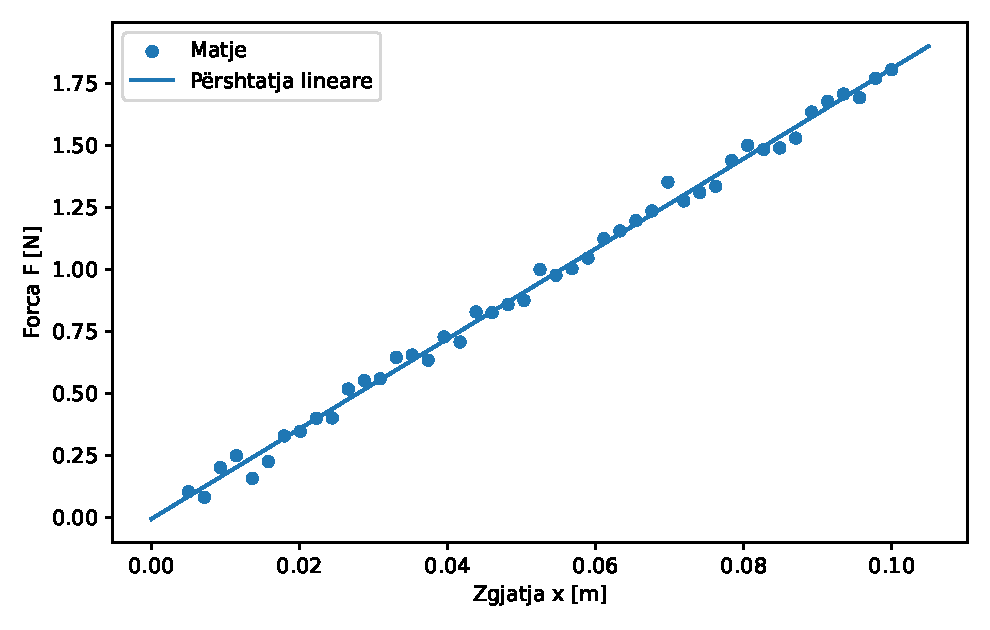
\includegraphics[width=.75\textwidth]{figures/fig_regresioni_hooke.pdf}\caption{Regresion linear për një eksperiment të tipit të ligjit të Hukut.}\label{fig:hooke}\end{figure}
Në notebook do të implementohen si zgjidhja me ekuacionet normale, ashtu edhe \texttt{LinearRegression}. Krahasimi duhet të përfshijë koeficientët, MSE, rezidualet dhe kohën e llogaritjes. Për të ilustruar stabilitetin numerik, një ushtrim shton një veçori pothuajse identike me $x$ dhe studion ndryshimin e koeficientëve.


\paragraph{Problem tipik në fizikë: përcaktimi i një konstante elastike.}
Për një sustë që punon në regjimin linear, ligji i Hukut jep $F=kx$. Nëse forca dhe zgjatja maten me zhurmë, pjerrësia e drejtës së përshtatur vlerëson $k$. Këtu regresioni nuk është thjesht një mjet parashikimi: koeficienti ka njësi dhe kuptim fizik. Rezidualet tregojnë nëse gabimi është në përputhje me zhurmën ose nëse shfaqet një devijim sistematik, për shembull sepse susta po del nga regjimi elastik.

\paragraph{Problem tipik jashtë fizikës: konsumi i energjisë së një ndërtese.}
Në një interval të kufizuar temperaturash, konsumi ditor për ngrohje mund të afrohet me një marrëdhënie lineare me temperaturën e jashtme. Një pjerrësi më e madhe në madhësi mund të sinjalizojë izolim më të dobët. Megjithatë, nëse modeli përdoret jashtë diapazonit të temperaturave të trajnimit, ekstrapolimi mund të dështojë sepse sistemi i ngrohjes hyn në regjim tjetër ose sepse sjellja e banorëve ndryshon.

\begin{figure}[H]\centering
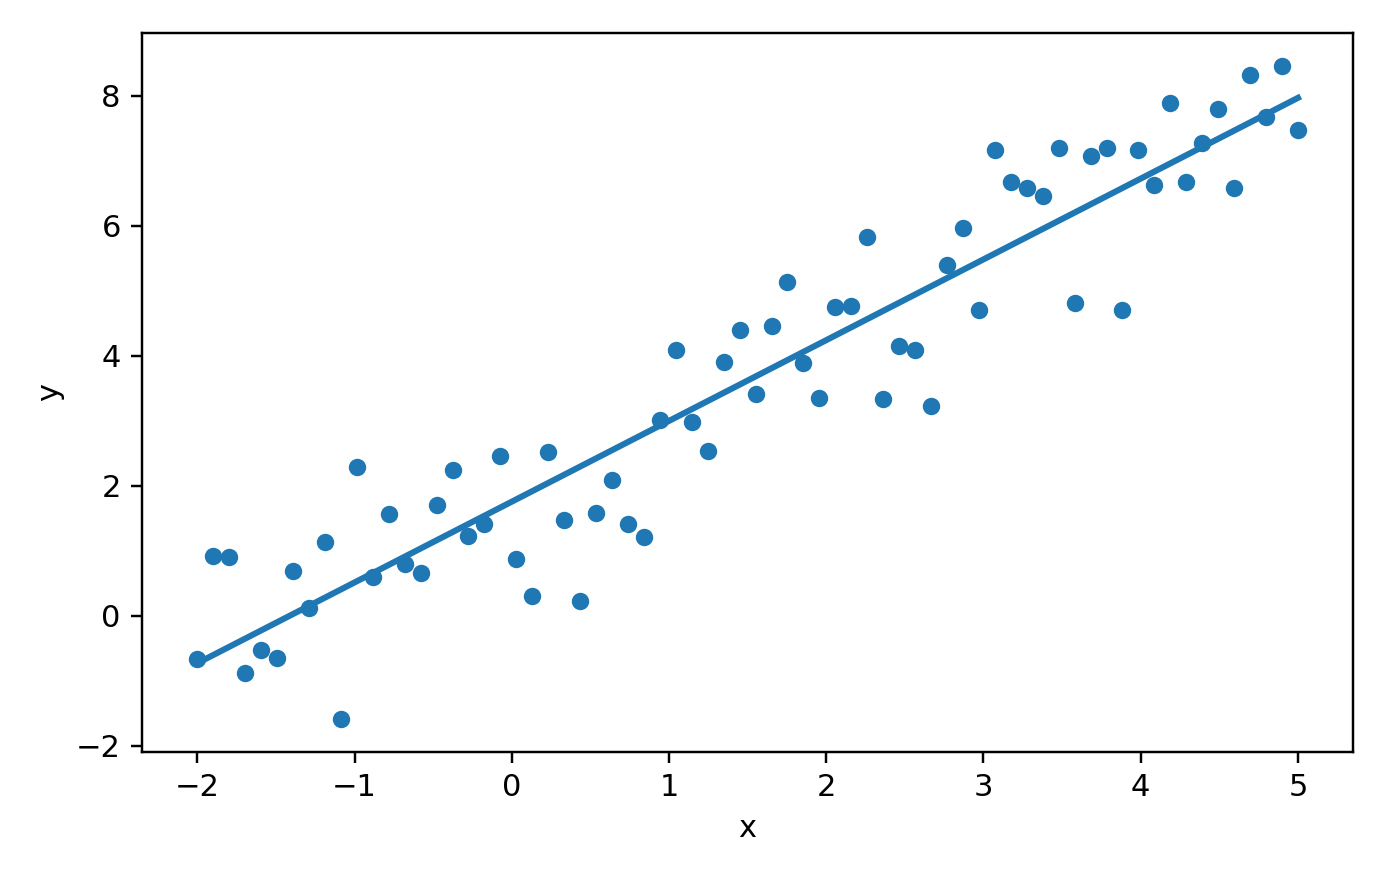
\includegraphics[width=.72\textwidth]{fig_regresion_linear_pd.png}
\caption{Ideja gjeometrike e regresionit linear. Rivizatim i përshtatur nga figura \emph{Linear regression.svg}, Sewaqu, Wikimedia Commons, domen publik. Burimi i lirë: \url{https://commons.wikimedia.org/wiki/File:Linear_regression.svg}.}
\end{figure}

\paragraph{Ilustrim me kod.}
\begin{lstlisting}
import numpy as np
X1 = np.c_[np.ones(len(x)), x]
beta = np.linalg.solve(X1.T @ X1, X1.T @ F)
F_hat = X1 @ beta
residuals = F - F_hat
print("k =", beta[1], "N/m")
\end{lstlisting}
Përdorimi i \texttt{solve} është numerikisht më i përshtatshëm se llogaritja e drejtpërdrejtë e inversit. Në laborator, kjo zgjidhje krahasohet me \texttt{LinearRegression}, por interpretimi fizik i koeficientit duhet të mbetet i njëjtë.

\section{Ushtrime dhe zgjerime}

\textbf{1.} Derivoni ekuacionet normale për modelin me intercept dhe një veçori duke përdorur derivime skalare. \textbf{2.} Tregoni se rezidualet janë ortogonale me kolonat e $X$. \textbf{3.} Për një eksperiment me pasiguri të njohura $\sigma_i$, shpjegoni pse peshat natyrore janë proporcionalisht $1/\sigma_i^2$. \textbf{4.} Krahasoni zgjidhjen nga inversi, \texttt{np.linalg.solve}, QR dhe pseudoinversi në një matricë keq të kondicionuar. \textbf{5.} Diskutoni dallimin midis pasigurisë së koeficientit dhe gabimit të parashikimit për një matje të re.


\paragraph{Regresioni si problem inverse.}
Në shumë eksperimente fizike regresioni linear është një formë e thjeshtë e problemit inverse: matim një përgjigje dhe duam të nxjerrim parametrat e modelit që e prodhojnë. Nëse matrica $X$ përmban kolona që janë shumë të ngjashme, të dhënat nuk mund të dallojnë mirë kontributet e parametrave përkatës. Kjo është çështje identifikueshmërie, jo vetëm çështje numerike. Numri i madh i kondicionimit i $X^TX$ paralajmëron se ndryshime të vogla në matje mund të prodhojnë ndryshime të mëdha në koeficientë. Për një fizikan, kjo do të thotë se dizajni i eksperimentit mund të jetë i pamjaftueshëm për të ndarë efektet.

Një shembull i thjeshtë është modeli $y=\beta_1x+\beta_2(x+\delta z)$ me $\delta\ll1$. Dy kolonat e dizajnit janë pothuajse të njëjta. Kombinimi $\beta_1+\beta_2$ mund të përcaktohet mirë, ndërsa koeficientët individualë mund të kenë pasiguri të mëdha. Një algoritëm mund të japë numra me shumë shifra, por këto shifra nuk përfaqësojnë informacion real. Raportimi i kovariancës së parametrave dhe i numrit të kondicionimit është prandaj pjesë e interpretimit fizik.

\paragraph{Reziduali si test i modelit.}
Nëse rezidualet tregojnë strukturë sistematike -- për shembull, pozitive në skaje dhe negative në mes -- supozimi i linearitetit është i dyshimtë. Nëse amplituda e rezidualeve rritet me $x$, kemi heteroskedasticitet; nëse rezidualet pasuese janë të korreluara, supozimi i pavarësisë është i dobët. Një vlerë e mirë e $R^2$ nuk e zëvendëson këtë diagnostikë. Në fizikë shpesh është më e vlefshme të shohim një devijim sistematik të vogël nga modeli sesa të përmirësojmë një metrikë globale.

\paragraph{Shembull i punuar: rënia e lirë.}
Për $s(t)=s_0+v_0t+\tfrac12gt^2$, nëse $s_0$ dhe $v_0$ nuk janë zero, regresioni vetëm ndaj $t^2$ do të prodhojë vlerësim të anshëm të $g$. Matrica e dizajnit duhet të përmbajë kolonat $1,t,t^2$. Koeficienti i $t^2$ është $g/2$. Ky shembull tregon rëndësinë e përfshirjes së termave fizikisht të nevojshëm dhe dallimin midis ``modelit linear'' dhe ``funksionit linear të kohës''.

Nëse koha ka pasiguri jo të neglizhueshme, modeli klasik OLS, i cili supozon hyrje pa gabim, nuk është më plotësisht adekuat. Kjo hap derën drejt metodave të regresionit me gabime në të dyja boshtet, por për këtë kurs mjafton të kuptohet kufiri i supozimit. Një manual i mirë duhet të tregojë jo vetëm formulën që përdoret, por edhe kur ajo pushon së qeni e përshtatshme.

\paragraph{Nga vlerësimi te parashikimi.}
Intervali i besimit për mesataren e parashikuar në një $x_0$ dhe intervali i parashikimit për një matje të re nuk janë e njëjta gjë. I pari përfshin pasigurinë e koeficientëve; i dyti përfshin edhe zhurmën e një vrojtimi të ri. Kështu intervali i parashikimit është më i gjerë. Ky dallim është thelbësor kur modeli përdoret për të vlerësuar një parametër fizik kundrejt rastit kur përdoret për të parashikuar matjen e ardhshme.

\chapter[Regresioni polinomial]{Regresioni polinomial dhe regularizimi}

Modelet reale rrallë mbeten lineare në të gjithë diapazonin e vëzhgimit. Megjithatë, kalimi nga një model linear në një model më fleksibël sjell menjëherë një pyetje më të thellë: sa kompleksitet është i justifikuar nga të dhënat? Ky kapitull e përdor regresionin polinomial si laborator konceptual për të parë se si një model mund të përshtatet gjithnjë e më mirë me të dhënat e trajnimit dhe, njëkohësisht, të bëhet më pak i besueshëm për të dhëna të reja.

Regularizimi shfaqet këtu jo si një truk numerik, por si një mënyrë për të formalizuar preferencën ndaj zgjidhjeve më të qëndrueshme. Në analizën fizike kjo lidhet natyrshëm me problemet inverse dhe me faktin se të dhënat e zhurmshme nuk justifikojnë gjithmonë liri të pakufizuara në model. Në aplikime të tjera, e njëjta ide mbron kundër modeleve që reagojnë tepër fort ndaj luhatjeve të rastësishme të tregut, sjelljes së konsumatorit ose sinjaleve biologjike.
\section{Nga lineariteti në parametra te jolineariteti në veçori}

Një model mund të jetë linear në parametra pa qenë vijë e drejtë në ndryshoren fizike. Regresioni polinomial i shkallës $m$ shkruhet
\[
\hat y=\beta_0+\beta_1x+\beta_2x^2+\cdots+\beta_mx^m.
\]
Duke ndërtuar matricën e dizajnit me kolonat $1,x,x^2,\ldots,x^m$, problemi mbetet regresion linear në koeficientë. Ky vëzhgim është i rëndësishëm sepse e ndan \emph{përfaqësimin} e veçorive nga algoritmi i përshtatjes.

Në kalibrimin e një sensori, një term kuadratik mund të përfaqësojë jolinearitet të butë të përgjigjes. Por shtimi mekanik i fuqive gjithnjë e më të larta mund ta bëjë modelin shumë fleksibël. Në këtë kapitull kompleksiteti nuk trajtohet si koncept abstrakt: ai shihet në ndryshimin e gabimit të trajnimit dhe validimit kur rritet shkalla e polinomit.

\section{Mbipërshtatja si fenomen i matshëm}

Nëse kemi $N$ pika dhe përdorim një polinom me shumë parametra, modeli mund të kalojë shumë afër çdo pike trajnimi. Kjo nuk do të thotë se kemi zbuluar ligjin fizik. Shumë nga kthesat e vogla mund të jenë përgjigje ndaj zhurmës. Kur matjet përsëriten, kthesat ndryshojnë fort: ky është manifestim i variancës së lartë.

Figura~\ref{fig:poly} krahason tre shkallë. Modeli i shkallës së parë ka anshmëri të dukshme; shkalla e dytë përputhet me mekanizmin gjenerues; shkalla e tetë është mjaft fleksibël për të ndjekur luhatje lokale. Vlerësimi duhet bërë me validim të kryqëzuar, jo duke zgjedhur modelin që duket më bukur në të njëjtat pika.
\begin{figure}[H]\centering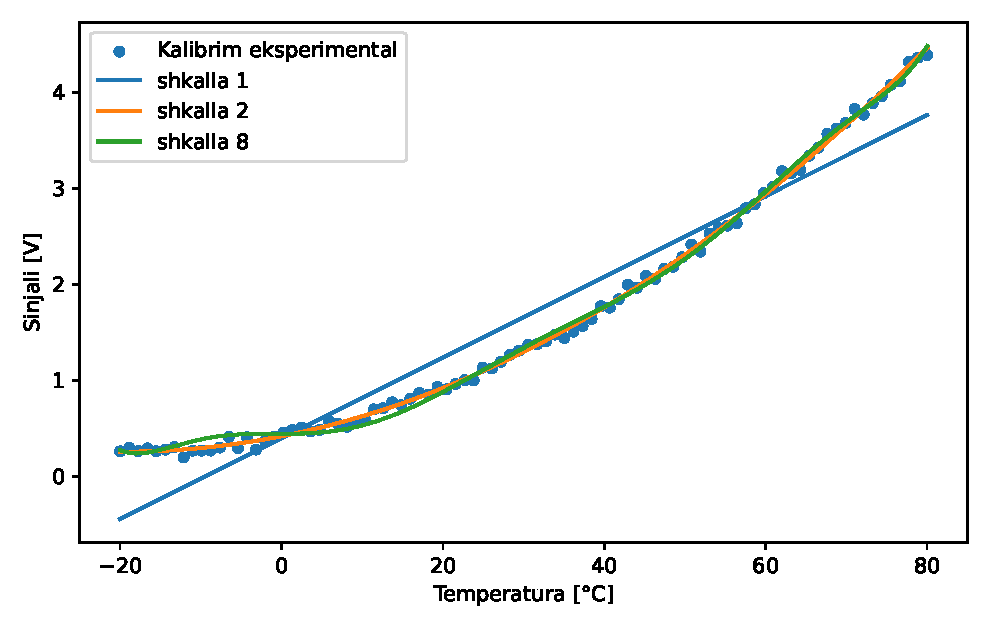
\includegraphics[width=.77\textwidth]{figures/fig_regresioni_polinomial.pdf}\caption{Kompleksiteti i modelit në një problem kalibrimi.}\label{fig:poly}\end{figure}

\section{Ridge: regularizim me normën $L_2$}

Regresioni Ridge minimizon
\[
\mathcal L(\boldsymbol\beta)=\|\mathbf y-X\boldsymbol\beta\|_2^2+\lambda\|\boldsymbol\beta\|_2^2,
\]
zakonisht pa penalizuar interceptin. Zgjidhja është
\[
\hat{\boldsymbol\beta}_{\rm Ridge}=(X^TX+\lambda I)^{-1}X^T\mathbf y.
\]

\paragraph{Interpretim.}
Ridge ndryshon jo vetëm madhësinë e koeficientëve, por edhe mënyrën se si modeli reagon ndaj drejtimeve të dobëta të të dhënave. Në një drejtim ku $X^TX$ ka vlerë vetjake të vogël, OLS mund të prodhojë një koeficient shumë të madh; shtesa $\lambda I$ e kufizon këtë amplifikim. Fizikisht, po pranojmë një sasi të vogël anshmërie për të fituar stabilitet dhe variancë më të ulët.
Termi $\lambda I$ stabilizon drejtimet ku $X^TX$ ka vlera vetjake të vogla. Kështu Ridge nuk është vetëm mjet statistik për mbipërshtatjen; është edhe regularizim numerik i një problemi inverse.

Hiperparametri $\lambda$ kontrollon kompromisin. Për $\lambda=0$ marrim OLS; për vlera shumë të mëdha koeficientët shtypen drejt zeros dhe modeli nënpërshtatet. Përzgjedhja e $\lambda$ duhet bërë brenda validimit, dhe nëse veçoritë kanë njësi shumë të ndryshme, standardizimi është thelbësor sepse penaliteti vepron mbi madhësinë numerike të koeficientëve.

\section{Lasso: sparsiteti dhe kufijtë e interpretimit}

Lasso zëvendëson normën kuadratike me normën $L_1$,
\[
\mathcal L(\boldsymbol\beta)=\|\mathbf y-X\boldsymbol\beta\|_2^2+\lambda\sum_j|\beta_j|.
\]
Gjeometria e penalitetit lejon që koeficientë të bëhen ekzaktësisht zero. Për këtë arsye Lasso përdoret shpesh edhe për përzgjedhje veçorish. Megjithatë, ``koeficient zero'' nuk do të thotë domosdoshmërisht ``madhësi fizikisht e parëndësishme''. Kur veçoritë janë fort të korreluara, Lasso mund të zgjedhë njërën në mënyrë jo stabile.

Në një problem fizik duhet të dallojmë interpretueshmërinë statistikore nga kauzaliteti. Një koeficient mund të jetë i dobishëm për parashikim pa përfaqësuar mekanizëm shkakor. Regularizimi është vendim mbi modelin dhe stabilitetin e tij, jo provë për ligj fizik.

\section{Krahasimi me pipeline dhe validim të kryqëzuar}

Një procedurë e pastër për polinome dhe regularizim është: krijim i veçorive polinomiale, standardizim, model Ridge/Lasso, dhe pastaj validim i kryqëzuar i gjithë zinxhirit. Nëse polinomet krijohen ose shkallëzohen duke parë gjithë bashkësinë, validimi nuk simulon më një eksperiment me të dhëna të panjohura.

Në notebook do të ndërtohet manualisht matrica Vandermonde, do të krahasohen OLS dhe Ridge për disa $\lambda$, dhe më pas do të përdoret \texttt{Pipeline}. Një kurbë validimi do të paraqesë gabimin ndaj shkallës së polinomit ose forcës së regularizimit. Ky është një shembull ku vizualizimi është mjet për të arsyetuar mbi kompromisin anshmëri--variancë.

Një eksperiment i vogël me kod e bën menjëherë të dukshëm rolin e kompleksitetit. Fragmenti i mëposhtëm mat njëkohësisht gabimin në trajnim dhe në validim për shkallë të ndryshme polinomiale:
\begin{lstlisting}[caption={Kompleksiteti polinomial dhe gabimi i validimit.}]
rows = []
for degree in range(1, 11):
    poly = PolynomialFeatures(degree, include_bias=False)
    Xtr = poly.fit_transform(x_train[:, None])
    Xva = poly.transform(x_valid[:, None])
    model = LinearRegression().fit(Xtr, y_train)
    rows.append((
        degree,
        mean_squared_error(y_train, model.predict(Xtr)),
        mean_squared_error(y_valid, model.predict(Xva))
    ))
\end{lstlisting}
Nëse gabimi i trajnimit vazhdon të bjerë, ndërsa ai i validimit fillon të rritet, kemi një shenjë tipike të mbipërshtatjes. Ky është argument empirik për zgjedhjen e kompleksitetit, jo thjesht një preferencë estetike për polinome më të ulëta.


\paragraph{Problem tipik në fizikë: kalibrimi jolinear i një sensori.}
Një sensor mund të ketë përgjigje afërsisht lineare pranë pikës së punës, por jolineare në të gjithë diapazonin. Një polinom i shkallës së dytë ose të tretë mund ta përshkruajë mirë kalibrimin. Nëse shkalla rritet shumë, modeli fillon të ndjekë zhurmën e pikave të kalibrimit dhe prodhon luhatje jo fizike midis tyre. Ridge e zbut këtë sjellje duke penalizuar koeficientët e mëdhenj.

\paragraph{Problem tipik jashtë fizikës: parashikimi i kërkesës.}
Kërkesa për energji, transport ose një produkt mund të ndryshojë jolinearisht me temperaturën, orën e ditës ose çmimin. Polinomet dhe veçoritë e zgjeruara japin fleksibilitet, por pa regularizim mund të krijojnë një model të paqëndrueshëm që reagon fort ndaj të dhënave të reja. Në këtë kontekst, parametri $\lambda$ kontrollon sa shumë i besojmë fleksibilitetit të modelit krahasuar me stabilitetin.

\paragraph{Ilustrim me kod.}
\begin{lstlisting}
from sklearn.preprocessing import PolynomialFeatures, StandardScaler
from sklearn.linear_model import Ridge
from sklearn.pipeline import make_pipeline

model = make_pipeline(PolynomialFeatures(6, include_bias=False),
                      StandardScaler(), Ridge(alpha=1.0))
model.fit(x[:, None], y)
\end{lstlisting}
Ky fragment duhet lexuar si përkthim i formulimit matematikor: gjenerohen veçori polinomiale, shkallëzohen dhe më pas koeficientët përcaktohen me penalizim $L_2$.

\section{Ushtrime}

\textbf{1.} Derivoni zgjidhjen e Ridge. \textbf{2.} Tregoni me dekompozim në vektorë vetjakë si regularizimi zvogëlon kontributin e drejtimeve të dobëta. \textbf{3.} Shpjegoni pse Lasso kërkon algoritëm iterativ ndërsa Ridge ka zgjidhje të mbyllur. \textbf{4.} Në një kalibrim sensori, krahasoni shkallët $1,2,4,8$ me të njëjtat fold-e. \textbf{5.} Jepni një shembull fizik ku ndërveprimi $x_1x_2$ është më i justifikuar se fuqitë e larta të një veçorie të vetme.


\paragraph{Kompleksiteti nuk është sinonim i jolinearitetit.}
Një model kuadratik me tre parametra mund të jetë më i thjeshtë se një model pjesë-pjesë me dhjetëra parametra, edhe pse të dy janë jolinearë në $x$. Në nxënien automatike kompleksiteti lidhet me aftësinë e klasës së modeleve për të përshtatur shumë konfigurime të ndryshme të të dhënave. Polinomi i shkallës së lartë ka shumë liri dhe mund të prodhojë oscilacione midis pikave. Ky fenomen lidhet me bazën monomiale $1,x,x^2,\ldots$, e cila mund të jetë keq e kondicionuar në intervale të gjera.

Në praktikë mund të përdoren baza ortogonale, splines ose transformime të tjera më stabile. Për kursin hyrës, polinomet janë të vlefshme sepse e bëjnë të dukshëm kompromisin midis bias dhe variance. Studentët duhet të shohin se gabimi i trajnimit bie pothuajse monotonisht me shkallën, ndërsa gabimi i validimit ka zakonisht minimum të ndërmjetëm.

\paragraph{Ridge si filtrim spektral.}
Le të shkruajmë $X^TX=V\Lambda V^T$. OLS shumëzon komponentin përgjatë drejtimit $v_j$ me $1/\lambda_j$. Nëse $\lambda_j$ është shumë e vogël, zhurma amplifikohet. Ridge zëvendëson këtë faktor me $1/(\lambda_j+\lambda)$, duke shtypur drejtimet e dobëta. Kjo lidh regularizimin me problemet inverse të fizikës, ku zgjidhjet e paqëndrueshme stabilizohen duke penalizuar norma ose derivime.

Ky interpretim tregon edhe çmimin e regularizimit: futet anshmëri. Koeficientët shtypen drejt zeros edhe kur vlera e vërtetë nuk është zero. Përfitimi është ulja e variancës dhe shpesh ulja e gabimit në të dhëna të reja. Nuk ka kontradiktë: qëllimi i parashikimit nuk është domosdoshmërisht koeficienti i paanshëm në çdo drejtim.

\paragraph{Lasso dhe përzgjedhja e veçorive.}
Penaliteti $L_1$ favorizon zgjidhje sparse. Kjo është tërheqëse kur kemi shumë veçori dhe duam model kompakt. Por në prani të dy veçorive pothuajse ekuivalente, Lasso mund të zgjedhë njërën dhe të heqë tjetrën në mënyrë të ndjeshme ndaj mostrës. Për interpretim fizik duhet kontrolluar stabiliteti i përzgjedhjes me bootstrap ose me fold-e të ndryshme. Një veçori që zgjidhet vetëm në 40\% të rimostrimeve nuk duhet paraqitur si zbulim i fortë.

\paragraph{Shembull i punuar: kalibrim me saturim.}
Nëse sensori ka përgjigje që fillon lineare dhe më pas ngopet, një polinom mund të japë përshtatje të mirë brenda intervalit të kalibrimit por sjellje katastrofike jashtë tij. Ky është dallimi midis interpolimit dhe ekstrapolimit. Për parashikim jashtë intervalit duhet një model i motivuar nga fizika e sensorit ose të paktën kufizime që respektojnë saturimin. Cross-validation i zakonshëm, që lë jashtë pika të shpërndara brenda të njëjtit interval, nuk teston aftësinë e ekstrapolimit.

\paragraph{Zgjedhja e hiperparametrave.}
Nëse zgjedhim njëkohësisht shkallën e polinomit dhe $\lambda$, kemi një hapësirë dy-dimensionale hiperparametrash. Grid search mund të përdoret, por duhet kujdes: sa më shumë konfigurime provojmë, aq më shumë mund të përshtatemi me zhurmën e validimit. Në projekte të vogla është e dobishme të kufizohet hapësira duke përdorur arsyetim fizik dhe të ruhet një test final i paprekur. Nested cross-validation është zgjidhja më rigoroze kur duam vlerësim të paanshëm të gjithë procesit të përzgjedhjes.

\chapter[Klasifikimi logjistik]{Klasifikimi dhe regresioni logjistik}

Klasifikimi ndryshon natyrën e pyetjes: nuk kërkojmë më një madhësi të vazhdueshme, por një vendim midis dy ose më shumë mundësive. Kjo e bën të domosdoshëm dallimin midis probabilitetit që prodhon modeli dhe vendimit që merret mbi bazën e tij. Regresioni logjistik është veçanërisht i dobishëm sepse e bën këtë dallim të dukshëm dhe ruan një lidhje të qartë me modelet lineare të kapitujve të mëparshëm.

Në një detektor grimcash, për shembull, mund të kërkojmë të dallojmë sinjalin nga sfondi duke përdorur amplitudën, gjerësinë e impulsit dhe energjinë e depozituar. Në një bankë, i njëjti formalizëm mund të përdoret për të vlerësuar probabilitetin e vonesës së një kredie. Në të dyja rastet modeli jep një probabilitet; pragu me të cilin ky probabilitet shndërrohet në vendim duhet të lidhet me koston dhe rrezikun e gabimeve.
\section{Nga parashikimi i një madhësie te vendimi midis klasave}

Në klasifikim ndryshorja objektiv është diskrete. Një shembull tipik në fizikën eksperimentale është dallimi midis sinjalit dhe sfondit. Për çdo ngjarje mund të masim amplitudën, kohën e ngritjes, gjerësinë e impulsit dhe energjinë. Objektivi $y\in\{0,1\}$ shënon klasën. Një model i mirë nuk duhet të prodhojë vetëm një etiketë; shpesh është më e dobishme të prodhojë një rezultat të vazhdueshëm që mund të interpretohet si probabilitet ose si rangim.

Regresioni logjistik modelon log-raportin e gjasave si funksion linear,
\[
\log\frac{p}{1-p}=\mathbf w^T\mathbf x+b,
\]
prandaj
\[
p(y=1\mid\mathbf x)=\sigma(\mathbf w^T\mathbf x+b),\qquad \sigma(z)=\frac{1}{1+e^{-z}}.
\]

\paragraph{Interpretim.}
Kombinimi linear $\mathbf w^T\mathbf x+b$ mund të marrë çdo vlerë reale, ndërsa funksioni sigmoid e shndërron atë në intervalin $(0,1)$. Kështu regresioni logjistik ndan dy role: pjesa lineare përcakton gjeometrinë e kufirit, ndërsa sigmoid-i i jep rezultatit një shkallë probabilitare. Kjo është arsyeja pse pragu i vendimit mund të ndryshohet pa ritrajnuar domosdoshmërisht modelin.
Kufiri $p=0.5$ është hiperplan linear, por pragu nuk është detyrimisht 0.5; ai duhet të lidhet me kostot e gabimeve dhe me objektivin shkencor.

\section{Maksimumi i gjasës dhe entropia e kryqëzuar}

Për shembuj të pavarur Bernoulli, gjasa është
\[
L(\mathbf w,b)=\prod_i p_i^{y_i}(1-p_i)^{1-y_i}.
\]
Maksimizimi i log-gjasës është ekuivalent me minimizimin e humbjes logaritmike
\[
\mathcal L=-\sum_i\left[y_i\log p_i+(1-y_i)\log(1-p_i)\right].
\]
Kjo \term{entropi e kryqëzuar}{cross-entropy} penalizon fort parashikimet shumë të sigurta dhe të gabuara. Ndryshe nga regresioni linear, nuk ka zgjidhje të thjeshtë të mbyllur për $\mathbf w$; përdoren metoda iterative si gradient descent, Newton ose zgjidhës të tjerë konveksë.

Lidhja me implementimin nga parimet e para është e drejtpërdrejtë. Në notebook, probabilitetet dhe gradienti përdoren për të përditësuar peshat në mënyrë iterative:
\begin{lstlisting}[caption={Bërthama numerike e regresionit logjistik me zbritje të gradientit.}]
def sigmoid(z):
    return 1.0 / (1.0 + np.exp(-z))

for _ in range(n_iter):
    p = sigmoid(X @ w + b)
    grad_w = X.T @ (p - y) / len(y)
    grad_b = np.mean(p - y)
    w -= eta * grad_w
    b -= eta * grad_b
\end{lstlisting}
Ky fragment shfaq qartë se ``trajnimi'' është një problem optimizimi. Biblioteka profesionale përdor zgjidhës më robustë dhe kontroll numerik më të mirë, por objekti matematik që optimizohet mbetet i njëjti.

Regularizimi $L_2$ shton zakonisht $\lambda\|\mathbf w\|^2$ dhe ndihmon kur veçoritë janë të shumta ose të korreluara. Në \texttt{scikit-learn}, parametrizimi shpesh përdor $C$, afërsisht invers të forcës së regularizimit: $C$ i madh do të thotë penalitet më i dobët.

\section{Metrikat e klasifikimit}

Matrica e konfuzionit ndan rezultatet në pozitivë të vërtetë, negativë të vërtetë, pozitivë të rremë dhe negativë të rremë. Prej saj llogariten
\[
\mathrm{precision}=\frac{TP}{TP+FP},\qquad
\mathrm{recall}=\frac{TP}{TP+FN},
\]
si dhe specifika $TN/(TN+FP)$. Metrika $F_1$ është mesatarja harmonike e precision dhe recall.

Në fizikën e ngjarjeve të rralla, këto madhësi kanë interpretim operacional. Rritja e ndjeshmërisë mund të rrisë kontaminimin nga sfondi. Nuk ka prag universal: zgjedhja duhet lidhur me analizën që do të bëhet pas klasifikimit. Kur rezultati i modelit është i vazhdueshëm, kurba ROC paraqet kompromisin midis ndjeshmërisë dhe normës së pozitivëve të rremë për të gjitha pragjet. AUC mat aftësinë e renditjes, jo cilësinë e kalibrimit të probabiliteteve.

\section{Kufiri i vendimit, shkallëzimi dhe interpretimi}

Koeficientët $w_j$ japin drejtimin e ndryshimit të log-odds për një rritje njësi të veçorisë $x_j$, duke mbajtur të tjerat konstante. Ky interpretim është i ndjeshëm ndaj njësive; standardizimi e bën më të lehtë krahasimin numerik të koeficientëve, por interpretimi fizik duhet kthyer në njësitë origjinale.

Në dy dimensione kufiri i vendimit mund të vizatohet drejtpërdrejt. Figura~\ref{fig:logdet} tregon dy veçori të impulsit të një detektori. Vija e modelit është kompromis statistikor; mbivendosja e klasave tregon se asnjë hiperplan nuk mund të ndajë çdo ngjarje pa gabim. Kjo është një situatë më realiste se shembujt artificialisht të ndashëm.
\begin{figure}[H]\centering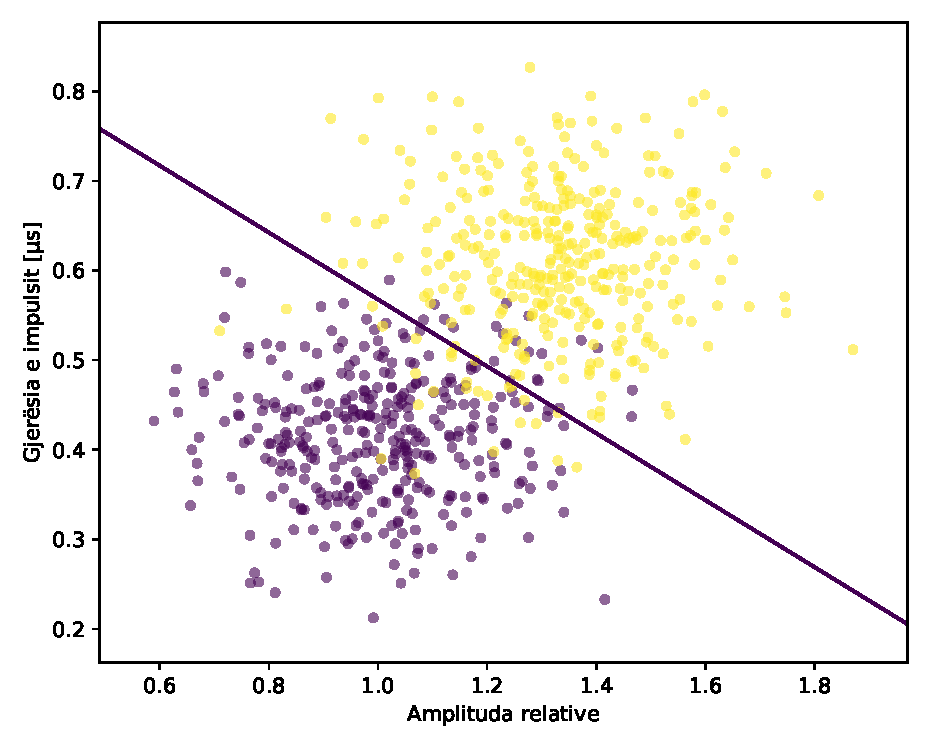
\includegraphics[width=.67\textwidth]{figures/fig_logistic_detector.pdf}\caption{Regresion logjistik për diskriminim sinjal--sfond.}\label{fig:logdet}\end{figure}

\section{ROC, kalibrimi dhe pragjet}

Figura~\ref{fig:roc} tregon një kurbë ROC për të njëjtin problem. Pika optimale nuk përcaktohet vetëm nga gjeometria e kurbës: ajo varet nga prevalenca e klasave dhe nga kostoja shkencore e gabimeve. Në një eksperiment kërkimi, mund të preferohet një prerje që ruan shumicën e sinjalit edhe me më shumë sfond; në një sistem alarmi mund të jetë e kundërta.
\begin{figure}[H]\centering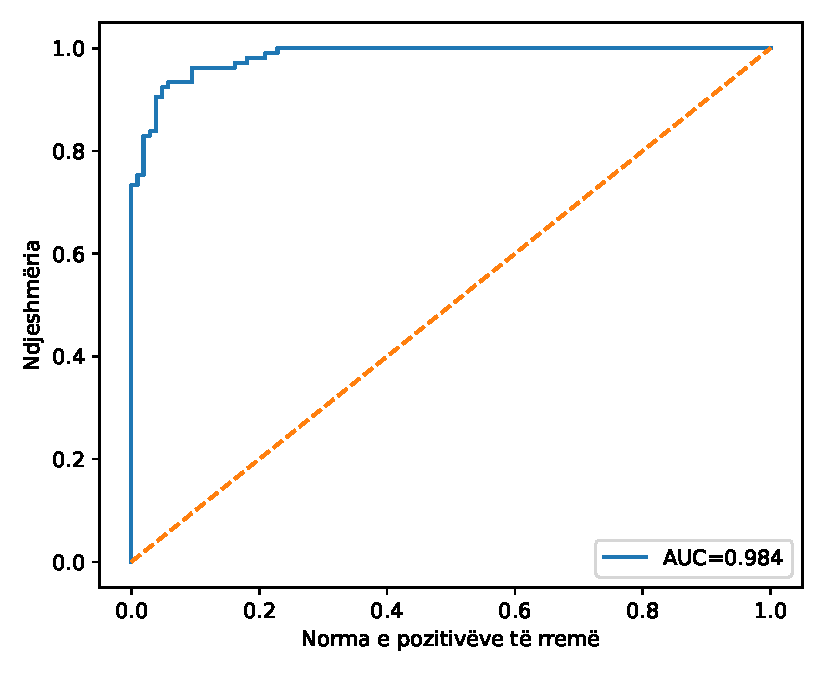
\includegraphics[width=.62\textwidth]{figures/fig_roc_detector.pdf}\caption{Kurba ROC për klasifikimin e pulseve.}\label{fig:roc}\end{figure}
Kalibrimi është pyetje tjetër: ndër ngjarjet të cilave modeli u jep probabilitet rreth 0.8, a janë afërsisht 80\% vërtet pozitive? Një model mund të ketë AUC të mirë por probabilitete të pakalibruara. Kjo dallim është i rëndësishëm kur probabilitetet futen në analiza të mëtejshme ose në vendime me kosto të ndryshme.


\paragraph{Problem tipik në fizikë: sinjal kundrejt sfondit.}
Supozoni se çdo impuls i një detektori përshkruhet nga energjia e depozituar dhe koha e ngritjes. Ngjarjet e sinjalit priren të zënë një zonë të caktuar të kësaj hapësire, por mbivendosen me sfondin. Regresioni logjistik nuk jep vetëm etiketën; ai jep një vlerësim të probabilitetit që ngjarja t'i përkasë klasës së sinjalit. Kjo lejon që pragu të zgjidhet në varësi të faktit nëse eksperimenti penalizon më fort pozitivët e rremë apo humbjen e sinjaleve reale.

\paragraph{Problem tipik jashtë fizikës: rreziku i mospagimit.}
Në një aplikim financiar, veçoritë mund të përfshijnë raportin borxh/të ardhura, historikun e pagesave dhe kohëzgjatjen e punësimit. Modeli prodhon një probabilitet mospagimi. Këtu një prag $0.5$ nuk ka ndonjë status të veçantë; ai duhet të zgjidhet sipas kostos së vendimeve dhe politikave të institucionit. Ky shembull e bën të qartë pse klasifikimi probabilistik dhe vendimi final janë dy hapa të ndryshëm.

\begin{figure}[H]\centering
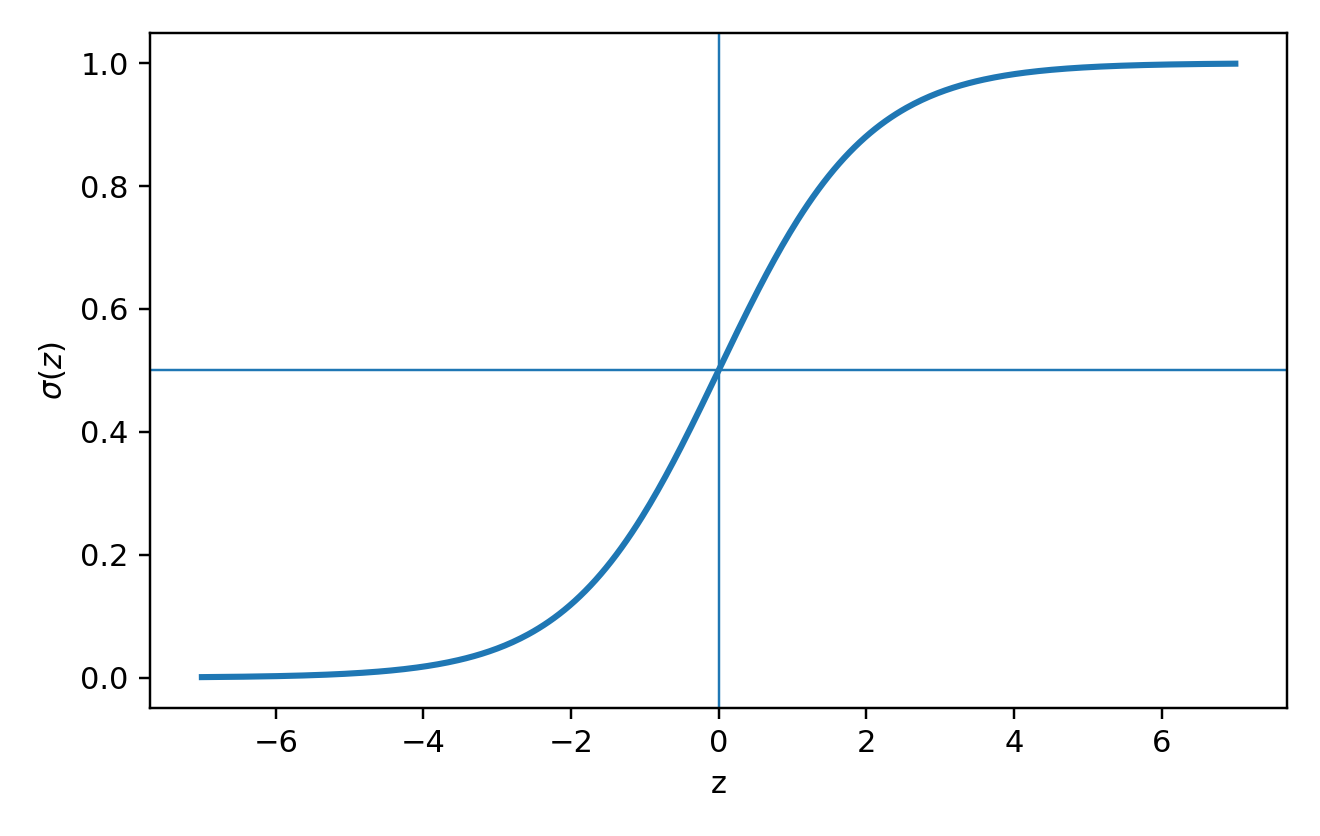
\includegraphics[width=.68\textwidth]{fig_logistike_cc0.png}
\caption{Funksioni logjistik dhe kalimi nga një madhësi reale $z$ te një vlerë në intervalin $(0,1)$. Rivizatim i përshtatur nga \emph{Logistische Funktion.svg}, Stefan Pohl, Wikimedia Commons, CC0. \url{https://commons.wikimedia.org/wiki/File:Logistische_Funktion.svg}.}
\end{figure}

\paragraph{Ilustrim me kod.}
\begin{lstlisting}
def sigmoid(z):
    return 1.0 / (1.0 + np.exp(-z))

p = sigmoid(X @ w + b)
y_hat = (p >= threshold).astype(int)
\end{lstlisting}
Ndryshimi i pragut (\texttt{threshold}) nuk ritrajnon modelin; ai ndryshon vetëm rregullin e vendimit. Ky dallim është thelbësor kur lexohen kurbat ROC dhe precision--recall.

\section{Ushtrime}

\textbf{1.} Derivoni gradientin e cross-entropy për regresionin logjistik. \textbf{2.} Për një matricë konfuzioni të dhënë, llogaritni accuracy, precision, recall, specificity dhe $F_1$. \textbf{3.} Jepni një problem ku AUC është e përshtatshme dhe një tjetër ku kalibrimi është më i rëndësishëm. \textbf{4.} Shpjegoni pse ndryshimi i pragut nuk ndryshon AUC. \textbf{5.} Ndërtoni një pipeline me standardizim dhe regresion logjistik dhe tregoni se standardizimi jashtë cross-validation krijon rrjedhje të vogël por reale informacioni.


\paragraph{Probabiliteti si objekt modelimi.}
Regresioni logjistik nuk modelon drejtpërdrejt klasën; ai modelon probabilitetin kushtor. Ky dallim lejon që i njëjti model të përdoret me pragje të ndryshme sipas qëllimit. Në një eksperiment ku ngjarjet pozitive janë të rralla por shumë të vlefshme, mund të preferohet recall i lartë. Në një sistem ku çdo alarm i rremë kushton shumë kohë instrumenti, precision mund të jetë më kritik. Pragu $0.5$ është thjesht një konventë kur kostot janë simetrike dhe prevalenca e trajnimit është përfaqësuese.

Nëse prevalenca në përdorim ndryshon nga ajo në trajnim, probabilitetet mund të mos jenë më të kalibruara. Kjo është një formë e ndryshimit të shpërndarjes. Një klasifikues mund të ruajë aftësinë e renditjes (AUC) dhe megjithatë të kërkojë rikalibrim të probabiliteteve.

\paragraph{Nga odds te koeficientët.}
Koeficienti $w_j$ interpretohet përmes faktorëve të odds: një rritje me një njësi e $x_j$ shumëzon odds me $\exp(w_j)$, duke mbajtur veçoritë e tjera fikse. Ky interpretim është i dobishëm por duhet kujdes kur veçoritë janë të korreluara. ``Mbajtja fikse'' e një madhësie ndërsa ndryshon një tjetër mund të mos jetë fizikisht e realizueshme. Për shembull, në një puls detektori amplituda dhe integrali mund të jenë të lidhura fort.

\paragraph{Klasat e pabalancuara.}
Kur pozitivët janë 1\% e të dhënave, accuracy është pothuajse e pakuptimtë. ROC mund të duket optimiste sepse norma e pozitivëve të rremë normalizohet me numrin e madh të negativëve. Kur klasa pozitive është e rrallë, kurba precision--recall shpesh është më informative. Baseline për precision është afërsisht prevalenca e klasës pozitive. Një precision prej 0.20 mund të jetë i dobët në një problem të balancuar, por shumë i mirë kur prevalenca është 0.01.

Peshimi i klasave ndryshon funksionin e humbjes dhe mund të ndihmojë modelin të kushtojë më shumë vëmendje klasës së rrallë. Megjithatë, peshat nuk krijojnë informacion të ri. Nëse veçoritë nuk dallojnë klasat, asnjë peshim nuk e zgjidh problemin.

\paragraph{Shembull i punuar: zgjedhja e pragut.}
Supozoni se kemi 10000 ngjarje, 200 sinjal dhe 9800 sfond. Në pragun A marrim recall 0.90 dhe false positive rate 0.05: kjo jep 180 sinjale të ruajtura por rreth 490 ngjarje sfondi. Precision është $180/(180+490)\approx0.27$. Në një prag B me recall 0.65 dhe FPR 0.005, ruajmë 130 sinjale dhe 49 sfond, me precision rreth 0.73. Cili është më i mirë? Përgjigjja varet nga analiza pasuese: nëse kemi metodë të fuqishme për heqjen e sfondit, A mund të jetë i preferueshëm; nëse çdo ngjarje e ruajtur kërkon analizë të kushtueshme, B mund të jetë më praktik.

\paragraph{Kalibrimi dhe besueshmëria.}
Një diagram kalibrimi ndan probabilitetet në intervale dhe krahason probabilitetin mesatar me frekuencën reale. Devijimi sistematik nga diagonalia tregon overconfidence ose underconfidence. Për vendime shkencore ku probabiliteti përdoret si peshë, kalibrimi është më i rëndësishëm se kur përdorim vetëm renditjen e ngjarjeve. Kjo është arsyeja pse performanca e një klasifikuesi nuk mund të përmblidhet me një metrikë të vetme.

\chapter[k-NN]{$k$ fqinjët më të afërt}

Metoda e fqinjëve më të afërt ofron një këndvështrim të ndryshëm nga modelet parametrike: në vend që të përmbledhë të dhënat në një numër të vogël koeficientësh, ajo ruan shembujt dhe vendos sipas afërsisë lokale. Pikërisht për këtë arsye, metoda është jashtëzakonisht intuitive, por edhe shumë e ndjeshme ndaj mënyrës se si maten distancat dhe ndaj numrit të dimensioneve.

Në fizikë kjo qasje është e natyrshme kur regjimet e një sistemi kanë nënshkrime të ngjashme në një hapësirë veçorish. Jashtë fizikës, një shembull klasik është njohja e modeleve të shkrimit të dorës: një simbol i ri krahasohet me shembuj të etiketuar dhe merr klasën e shumicës së fqinjëve. Thjeshtësia e algoritmit nuk duhet të fshehë pyetjet e rëndësishme mbi shkallëzimin, densitetin e pikave dhe kuptimin e metrikës së zgjedhur.
\section{Ideja lokale e të nxënit}

Metoda e \term{$k$ fqinjëve më të afërt}{$k$-nearest neighbours, k-NN} nuk ndërton një funksion parametrik global gjatë trajnimit. Ajo ruan shembujt dhe, për një pikë të re, kërkon $k$ pikat më të afërta sipas një metrike. Në klasifikim përdoret vota e shumicës; në regresion mesatarja ose një mesatare e ponderuar. Kjo e bën metodën konceptualisht të thjeshtë, por jo triviale: gjithçka varet nga çfarë do të thotë ``afër''.

Për distancën Euklidiane,
\[
d(\mathbf x,\mathbf z)=\sqrt{\sum_j(x_j-z_j)^2}.
\]

\paragraph{Interpretim.}
Distanca Euklidiane supozon se një ndryshim numerik me të njëjtën madhësi ka peshë të krahasueshme në çdo drejtim të hapësirës së veçorive. Ky supozim është i arsyeshëm vetëm pasi njësitë dhe shkallët janë trajtuar me kujdes. Në këtë kuptim, zgjedhja e metrikës është pjesë e modelimit fizik: ajo përcakton cilat gjendje quhen të ngjashme.
Nëse një veçori matet në mijëra njësi dhe një tjetër në të dhjetat, e para dominon distancën. Prandaj shkallëzimi është pjesë e modelit, jo një detaj kozmetik.

\section{Roli i $k$ dhe kompromisi lokal}

Me $k=1$, kufiri i vendimit është shumë i ndjeshëm ndaj çdo pike trajnimi; varianca është e lartë. Me $k$ shumë të madh, modeli mesatarizon rajone të gjera dhe mund të humbasë strukturë lokale; anshmëria rritet. Zgjedhja e $k$ është prandaj një shembull i qartë i kompromisit anshmëri--variancë dhe duhet bërë me validim.

Në klasifikim mund të përdoren pesha $1/d$ që u japin më shumë ndikim fqinjëve shumë të afërt. Por kjo rrit ndjeshmërinë ndaj pikave jashtëzakonisht pranë për shkak të zhurmës. Zgjedhja e metrikës dhe e peshave duhet të lidhet me gjeometrinë e problemit fizik.

Algoritmi bazë mund të shkruhet me pak rreshta, gjë që e bën k-NN veçanërisht të përshtatshëm për implementim didaktik:
\begin{lstlisting}[caption={Një hap i klasifikimit k-NN nga parimet e para.}]
d = np.sqrt(((X_train - x_new)**2).sum(axis=1))
idx = np.argsort(d)[:k]
labels = y_train[idx]
prediction = np.bincount(labels).argmax()
\end{lstlisting}
Në këtë fragment nuk ka fazë ``fit'' në kuptimin parametrik. Kostoja shtyhet te parashikimi, sepse duhet të llogariten distancat ndaj shumë pikave të trajnimit. Kjo shpjegon njëkohësisht thjeshtësinë dhe kufizimin llogaritës të metodës.

\section{Mallkimi i dimensionalitetit}

Në dimension të lartë, vëllimi rritet aq shpejt sa që një mostër e fundme bëhet e rrallë. Distanca te fqinji më i afërt dhe te pikat e largëta bëhen relativisht më të ngjashme; nocioni i lokalitetit dobësohet. Kjo është një formë e \term{mallkimit të dimensionalitetit}{curse of dimensionality}.

Për fiziken kjo ka pasoja praktike: shtimi i çdo veçorie të mundshme nuk është domosdoshmërisht përmirësim. Veçoritë pa informacion mund të prishin distancat dhe të ulin performancën e k-NN. Reduktimi dimensional, përzgjedhja e veçorive ose ndërtimi i madhësive me kuptim fizik mund të jetë më i vlefshëm se rritja e kompleksitetit të klasifikuesit.

\section{Shembull fizik: regjimet e një sistemi të zbehur}

Në bashkësinë sintetike të laboratorit çdo shembull përfaqëson një realizim të një sistemi oscilues dhe përshkruhet me frekuencën dominante dhe koeficientin e zbehjes. Tre regjime dinamike formojnë rajone të dallueshme, por me mbivendosje. Figura~\ref{fig:knn} e bën të dukshme pse një model lokal është i arsyeshëm.
\begin{figure}[H]\centering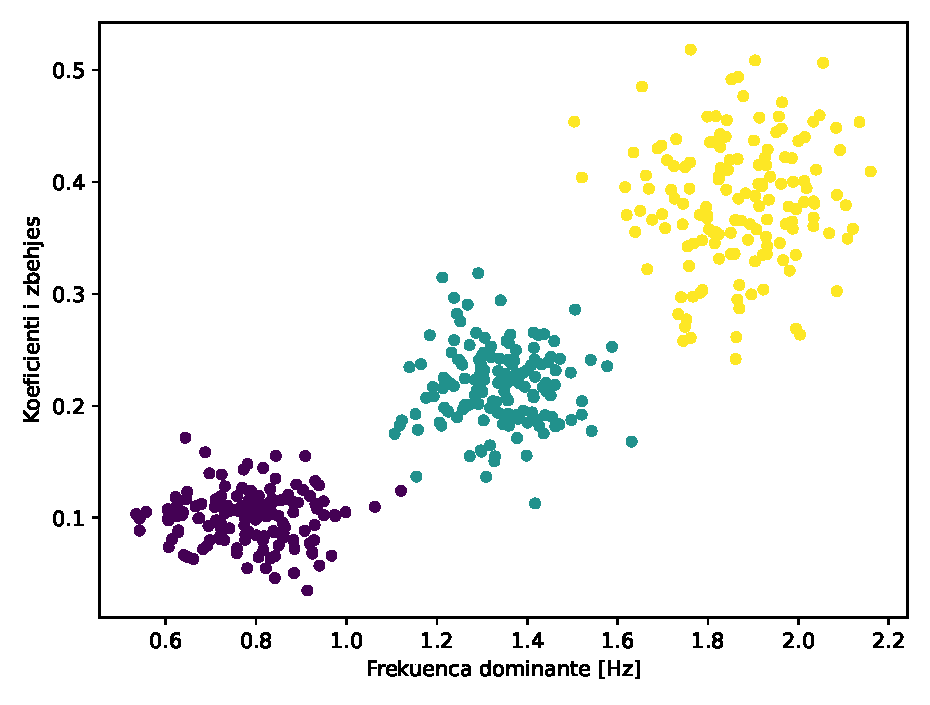
\includegraphics[width=.68\textwidth]{figures/fig_knn_regjime.pdf}\caption{Veçori të nxjerra nga regjime dinamike të ndryshme.}\label{fig:knn}\end{figure}
Notebook-u do të implementojë kërkimin manual të fqinjëve me NumPy, votimin dhe një kurbë të performancës ndaj $k$. Pastaj rezultatet krahasohen me \texttt{KNeighborsClassifier}. Një variant i ushtrimit shumëzon një nga veçoritë me 1000 për të demonstruar efektin e mungesës së standardizimit.

\section{Kostoja llogaritëse dhe kufijtë praktikë}

Trajnimi i k-NN është pothuajse ruajtje e të dhënave, por parashikimi kërkon krahasim me shumë ose të gjitha pikat e trajnimit. Për $N$ të madh dhe dimension $d$, kjo mund të kushtojë $O(Nd)$ për shembull të ri. Struktura si k-d trees mund të ndihmojnë në dimension të ulët, por humbin efikasitet në dimension të lartë.

Përparësia është transparenca: mund të shohim fqinjët që prodhuan vendimin. Kjo është formë e interpretueshmërisë lokale. Kufizimi është se një fqinj i afërt numerikisht nuk është domosdoshmërisht i ngjashëm fizikisht nëse metrika nuk përfaqëson mirë problemin.


\paragraph{Problem tipik në fizikë: identifikimi i regjimeve dinamike.}
Nga një seri kohore mund të nxirren veçori të tilla si energjia mesatare, frekuenca dominante dhe një masë e çrregullsisë. Nëse simulime të mëparshme kanë etiketa për regjime periodike dhe kaotike, një vrojtim i ri mund të klasifikohet sipas fqinjëve më të afërt. Pyetja kryesore është nëse distanca në këtë hapësirë veçorish ka kuptim fizik; nëse një veçori matet në një shkallë shumë më të madhe, ajo mund të dominojë vendimin.

\paragraph{Problem tipik jashtë fizikës: njohja e karaktereve të shkruara me dorë.}
Çdo imazh mund të paraqitet si një vektor pikselash ose veçorish. Një karakter i ri klasifikohet duke parë karakteret më të ngjashme në bashkësinë e trajnimit. Metoda funksionon mirë kur shembujt e ngjashëm ndodhen afër, por bëhet e kushtueshme kur numri i shembujve është i madh dhe më pak informative kur dimensioni rritet shumë.

\begin{figure}[H]\centering
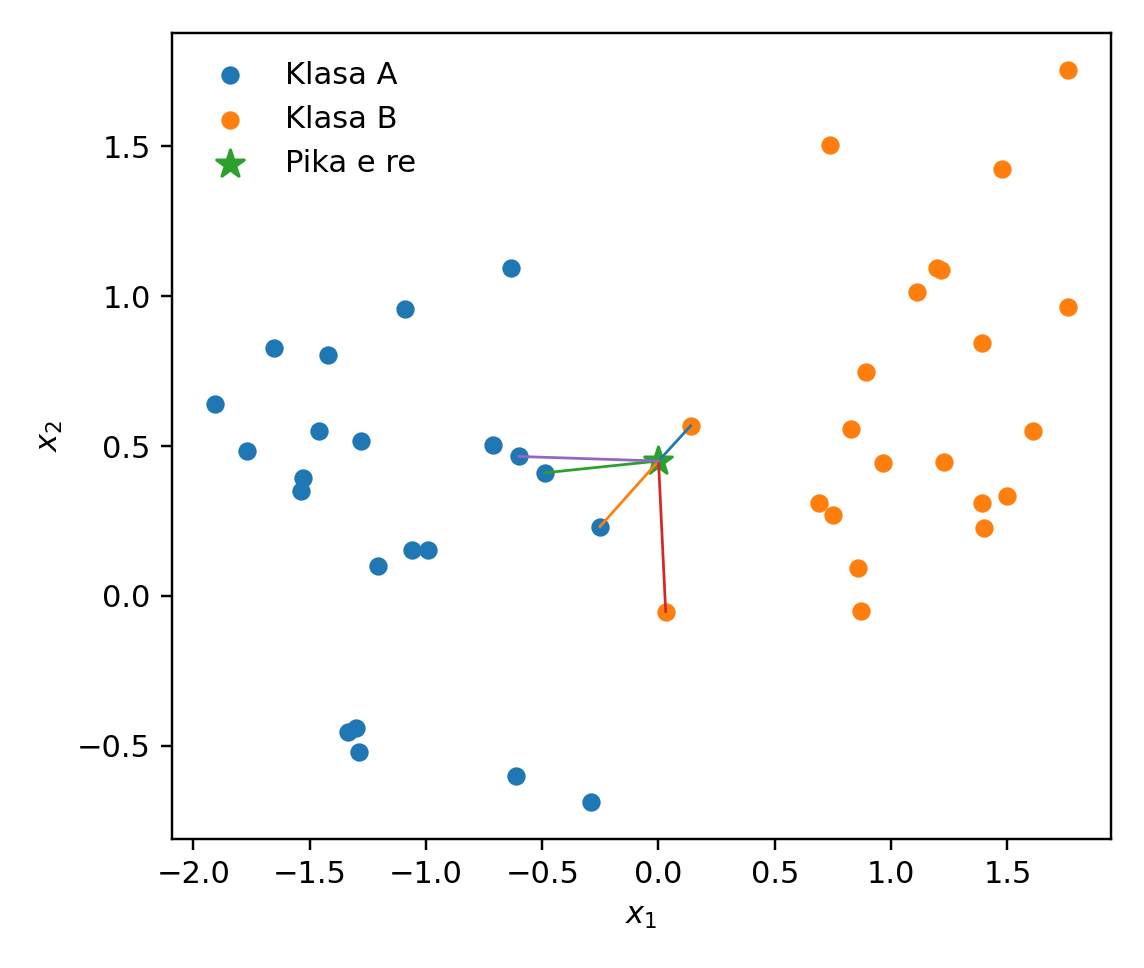
\includegraphics[width=.64\textwidth]{fig_knn_cc0_adapted.png}
\caption{Interpretim lokal i fqinjëve më të afërt. Rivizatim i përshtatur nga materiale të lira mbi grafët e fqinjit më të afërt, David Eppstein, Wikimedia Commons, CC0. \url{https://commons.wikimedia.org/wiki/File:Nearest_neighbor_graph.svg}.}
\end{figure}

\begin{lstlisting}
d = np.sqrt(((X_train - x_new)**2).sum(axis=1))
idx = np.argsort(d)[:k]
pred = np.bincount(y_train[idx]).argmax()
\end{lstlisting}
Këto tri rreshta përmbajnë të gjithë bërthamën e algoritmit. Çdo zgjerim praktik --- peshimi sipas distancës, kërkimi efikas ose zgjedhja e metrikës --- ndërtohet mbi këtë ide lokale.

\section{Ushtrime}

\textbf{1.} Implementoni k-NN pa \texttt{sklearn} dhe verifikoni barazinë e parashikimeve në një bashkësi të vogël. \textbf{2.} Studioni $k=1,3,5,15,50$ me të njëjtat fold-e. \textbf{3.} Shtoni pesë veçori zhurme dhe matni degradimin. \textbf{4.} Krahasoni distancën Euklidiane dhe Manhattan për një problem të shkallëzuar. \textbf{5.} Shpjegoni pse k-NN nuk ekstrapolon në kuptimin e zakonshëm të regresionit.


\paragraph{Gjeometria e distancës.}
Distanca Euklidiane supozon se të gjitha drejtimet në hapësirën e veçorive janë të krahasueshme pas shkallëzimit. Por në fizikë mund të ketë korrelacione të forta. Nëse dy veçori lëvizin së bashku, një metrikë Mahalanobis, që përdor kovariancën, mund të jetë më e përshtatshme. Megjithatë, vlerësimi i kovariancës në dimension të lartë është vetë problem statistik. Për kursin hyrës, standardizimi + Euclidean është baseline i mirë, por studentët duhet të dinë se ``metrika'' është pjesë e modelit.

\paragraph{Pse dimensioni i lartë është i vështirë.}
Në një hiperkub njësi, vëllimi i një topi me rreze të vogël zë pjesë gjithnjë e më të vogël të hapësirës kur dimensioni rritet. Për të mbajtur të njëjtën pjesë të të dhënave brenda një lagjeje, rrezja duhet të rritet. Kështu ``lokaliteti'' bëhet më pak lokal. Një mënyrë empirike për ta parë është të llogaritet raporti $d_{\max}/d_{\min}$ për një pikë reference: në dimension të lartë ky raport afrohet me 1 për shumë shpërndarje.

Ky fenomen shpjegon pse shtimi i veçorive zhurme dëmton k-NN. Çdo dimension shton variacion të parëndësishëm në distancë dhe mund të mbulojë sinjalin e dimensioneve informative. Përzgjedhja e veçorive dhe PCA mund të ndihmojnë, por duhet bërë vetëm nga trajnimi.

\paragraph{k-NN në regresion.}
Për një objektiv të vazhdueshëm, parashikimi mund të jetë mesatarja e $y$ të $k$ fqinjëve. Me $k=1$ marrim një funksion pjesë-pjesë që kalon nëpër vlerat e trajnimit; me $k$ të madh marrim sipërfaqe më të lëmuar. Ky është analog i qartë i bias--variance. Peshat sipas distancës mund të japin lëmim më lokal.

Në një problem të kalibrimit, k-NN regression është i aftë të interpoljë forma jolineare pa specifikuar polinom. Por jashtë diapazonit të të dhënave ai nuk ka mekanizëm të besueshëm ekstrapolimi: parashikimi mbetet afër vlerave të fqinjëve më të afërt në skaj. Kjo duhet ta bëjë studentin të mendojë për domenin e përdorimit.

\paragraph{Shembull i punuar: klasifikimi i regjimeve.}
Supozoni se frekuenca dhe zbehja janë standardizuar. Për një pikë të re $z=(0.4,-0.2)$ në koordinata standarde, pesë fqinjët më të afërt kanë etiketa $[0,0,1,0,1]$. k-NN me $k=5$ jep klasën 0. Nëse dy fqinjët e klasës 1 janë shumë më afër se tre të klasës 0, votimi me peshë distance mund të ndryshojë rezultatin. Kjo tregon se rregulli i agregimit është hiperparametër po aq sa $k$.

\paragraph{Diagnostika praktike.}
Për k-NN duhet të kontrollohen: kurba e validimit ndaj $k$; ndikimi i scaling; ndikimi i veçorive zhurme; stabiliteti i rezultatit ndaj metrikës; dhe kostoja e parashikimit. Nëse modeli do të përdoret online me miliona shembuj trajnimi, një metodë tjetër mund të jetë më praktike edhe kur accuracy është pak më e ulët.

\chapter[Pemët dhe ansamblet]{Pemët e vendimit dhe ansamblet}

Pemët e vendimit përkthejnë një problem shumëpërmasor në një varg pyetjesh lokale. Kjo i bën ato të lexueshme dhe shpesh tërheqëse në aplikime ku përdoruesi duhet të kuptojë pse u mor një vendim. Megjithatë, një pemë e vetme mund të ndryshojë ndjeshëm edhe kur të dhënat ndryshojnë pak; kjo paqëndrueshmëri është arsyeja pse metodat ansambël, veçanërisht pylli i rastësishëm, kanë një rol kaq të rëndësishëm.

Në fizikën e materialeve një pemë mund të ndajë faza sipas temperaturës, presionit dhe disa observablave mikroskopikë. Në sigurime, një pemë mund të përdorë moshën, historikun e dëmeve dhe karakteristika të policës për të ndarë profile rreziku. Në të dyja rastet është thelbësore të dallojmë interpretueshmërinë e një ndarjeje nga një pretendim shkakësor: fakti që një veçori përdoret lart në pemë nuk provon se ajo shkakton rezultatin.
\section{Ndarje rekursive e hapësirës së veçorive}

Një pemë vendimi e shndërron problemin e klasifikimit në një varg pyetjesh të tipit ``a është $x_j<t$?''. Çdo ndarje synon të krijojë nëngrupe më homogjene. Kjo e bën modelin të lexueshëm, por edhe shumë fleksibël: pa kufizime, pema mund të ndjekë deri edhe luhatjet aksidentale të mostrës.

Një \term{pemë vendimi}{decision tree} ndërton rregulla të formës $x_j<t$ dhe ndan në mënyrë rekursive të dhënat. Rezultati është një ndarje pjesë-pjesë e hapësirës së veçorive. Ndryshe nga regresioni logjistik, kufiri nuk është domosdoshmërisht linear dhe shkallëzimi i veçorive zakonisht nuk është i nevojshëm.

Në çdo nyje kërkohet ndarja që ul më shumë papastërtinë. Për klasifikim binar, \term{papastërtia Gini}{Gini impurity} është
\[
G=1-\sum_k p_k^2,
\]
ndërsa entropia është $H=-\sum_k p_k\log p_k$. Ndarja e mirë prodhon nyje fëmijë më homogjene se nyja prind. Kjo procedurë greedy nuk garanton pemën globalisht optimale, por është efikase dhe interpretuese.

\section{Thellësia, krasitja dhe mbipërshtatja}

Një pemë pa kufizime mund të vazhdojë ndarjet derisa gjethet të përmbajnë shumë pak pika. Gabimi i trajnimit bie, por varianca rritet. Hiperparametra si \texttt{max\_depth}, \texttt{min\_samples\_leaf} dhe krasitja me kosto-kompleksitet kontrollojnë këtë fleksibilitet.

Pemët janë një shembull i mirë për të parë se kompleksiteti nuk matet vetëm me numrin e parametrave. Struktura diskrete e ndarjeve dhe numri i gjetheve përcaktojnë sa forma të ndryshme mund të përfaqësojë modeli. Validimi i kryqëzuar duhet të përdoret për të zgjedhur thellësinë, jo grafiku i trajnimit.

\section{Bagging dhe pylli i rastësishëm}

\term{Bagging}{bagging} ndërton shumë modele mbi mostra bootstrap dhe mesatarizon parashikimet. Nëse gabimet e pemëve individuale nuk janë plotësisht të korreluara, mesatarizimi ul variancën. \term{Pylli i rastësishëm}{random forest} shton një burim tjetër rastësie: në çdo ndarje konsiderohet vetëm një nënbashkësi e veçorive. Kjo de-korrelon pemët dhe shpesh përmirëson ansamblin.

Random forest është model i fuqishëm bazë për të dhëna tabelare: kap jolinearitete dhe ndërveprime pa kërkuar shkallëzim. Por interpretimi i ``rëndësisë së veçorive'' duhet bërë me kujdes. Importanca e bazuar në impurity mund të favorizojë veçori me shumë vlera të mundshme. Permutation importance jep një alternativë më të lidhur me humbjen e performancës kur një veçori prishet.

\section{Boosting si ndërtim sekuencial}

Në boosting, modelet bazë ndërtohen sekuencialisht dhe fokusi zhvendoset te shembujt ose rezidualet që modeli aktual i shpjegon dobët. AdaBoost rrit peshën e shembujve të klasifikuar gabim; gradient boosting e interpreton procesin si zbritje gradienti në hapësirën e funksioneve.

Në këtë kurs boosting trajtohet konceptualisht dhe praktikisht, pa hyrë në të gjithë teorinë e optimizimit funksional. Qëllimi është të kuptohet dallimi midis ansambleve paralelë të tipit bagging dhe ndërtimit sekuencial të boosting, si dhe rreziku i hiperparametrave të shumtë në një kurs të shkurtër.

\section{Shembull: klasifikimi i fazave të materialit}

Bashkësia sintetike përdor densitetin, përçueshmërinë dhe fortësinë për të dalluar tre faza. Një pemë e cekët prodhon rregulla të lexueshme; një random forest rrit stabilitetin. Figura~\ref{fig:rfimp} paraqet importancat e një pylli, por ato duhen parë si tregues të modelit, jo si prova kauzale.
\begin{figure}[H]\centering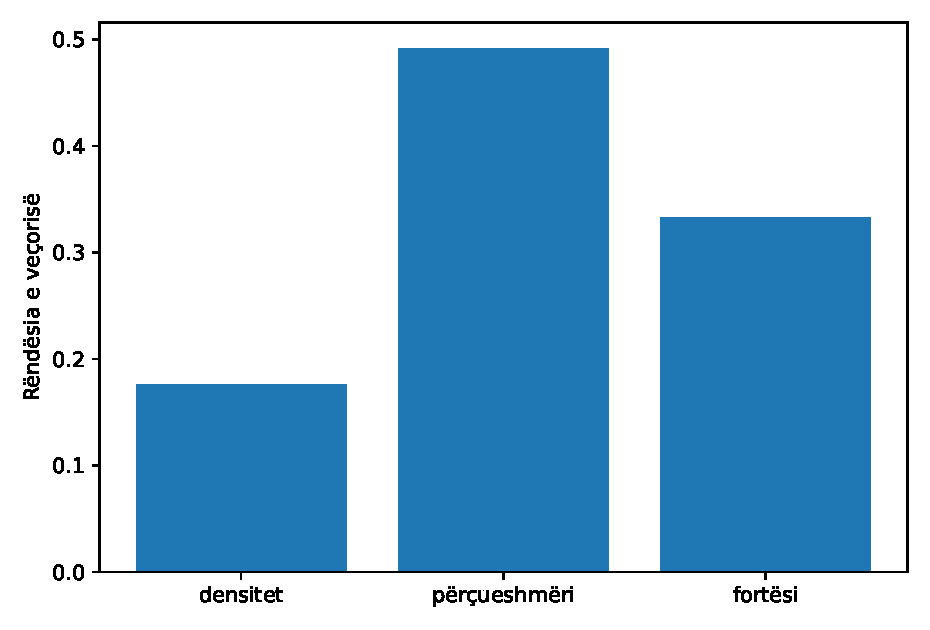
\includegraphics[width=.66\textwidth]{figures/fig_random_forest_importances.pdf}\caption{Rëndësi veçorish nga një random forest në një shembull materialesh.}\label{fig:rfimp}\end{figure}
Në notebook do të llogariten manualisht Gini dhe fitimi i një ndarjeje të vetme, pastaj do të përdoret \texttt{DecisionTreeClassifier}. Për random forest, implementimi i plotë manual nuk është objektiv pedagogjik; në vend të tij do të ndërtohet një bagging minimal me disa pemë dhe do të krahasohet me bibliotekën.


\paragraph{Problem tipik në fizikë: klasifikimi i fazave të një materiali.}
Një bashkësi simulimesh mund të përshkruhet nga temperatura, magnetizimi, susceptibiliteti dhe energjia. Një pemë vendimi kërkon pragje që ndajnë hapësirën në rajone gjithnjë e më homogjene. Nëse pema bëhet shumë e thellë, mund të mësojë luhatje statistikore të simulimeve individuale; një pyll i rastësishëm e redukton këtë variancë duke mesatarizuar shumë pemë të ndryshme.

\paragraph{Problem tipik jashtë fizikës: vlerësimi i rrezikut të një kërkese sigurimi.}
Një pemë mund të bëjë pyetje të tipit ``a ka pasur dëme të mëparshme?'', ``është vlera e pronës mbi një prag?'' ose ``sa është kohëzgjatja e policës?''. Struktura është e kuptueshme për një ekspert, por kjo nuk duhet ngatërruar me shkakësi. Ansambli përmirëson stabilitetin, ndërsa interpretimi zhvendoset nga një pemë e vetme te rëndësia mesatare e veçorive dhe analiza e parashikimeve.

\begin{figure}[H]\centering
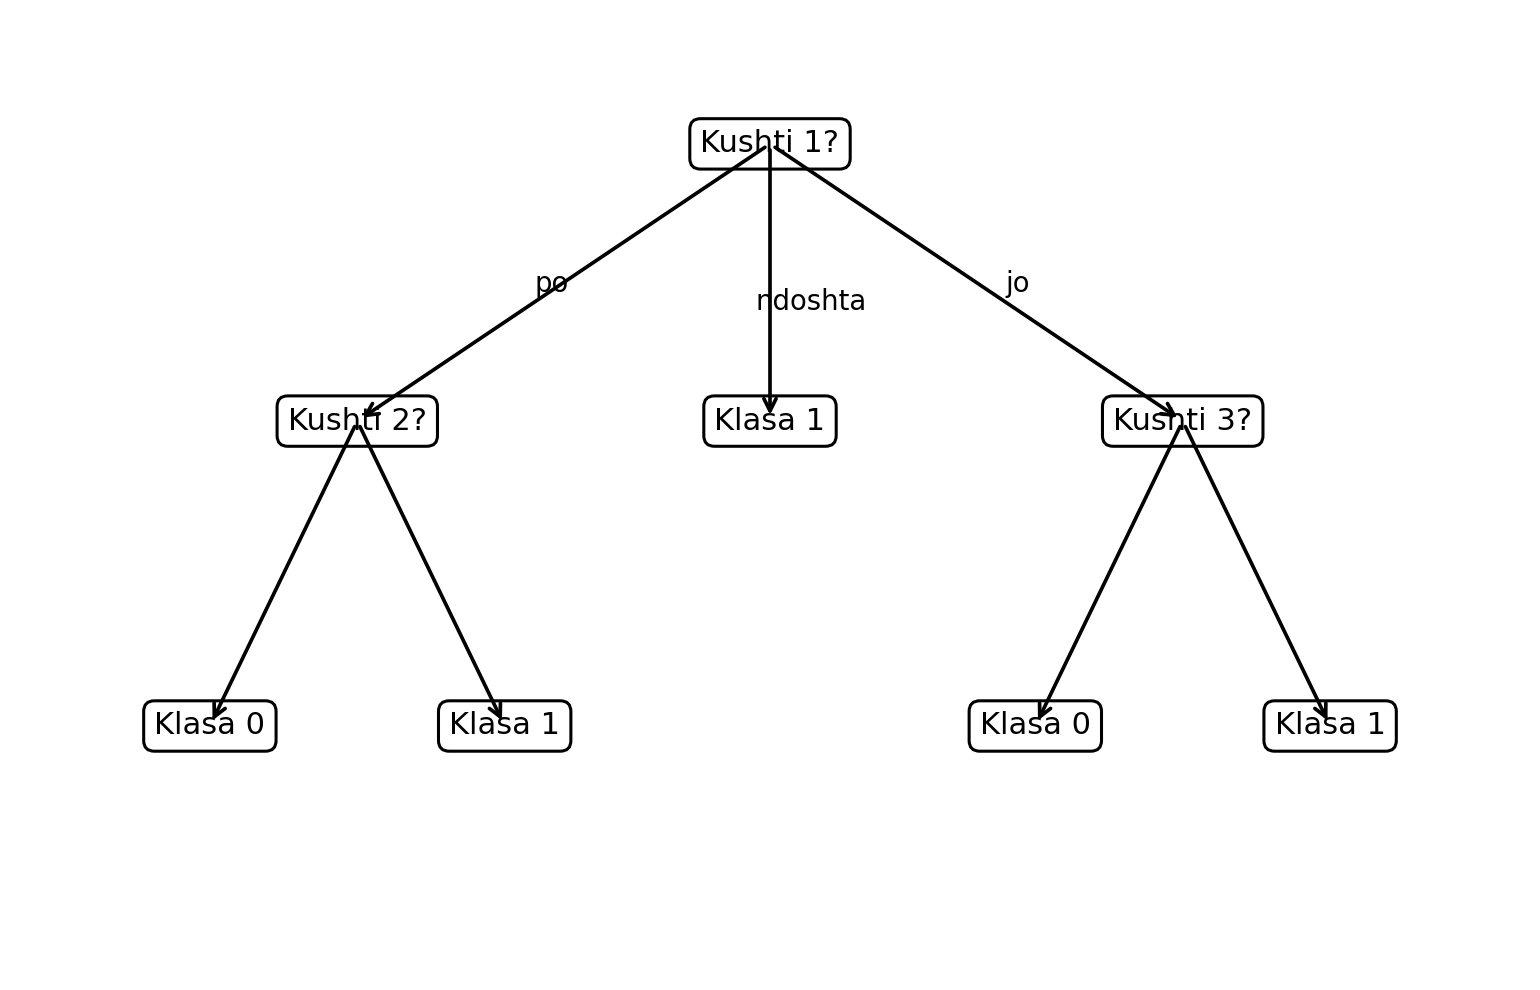
\includegraphics[width=.78\textwidth]{fig_peme_vendimi_pd_adapted.png}
\caption{Struktura bazë e një peme vendimi. Rivizatim i përshtatur nga \emph{Decision tree model.png}, T-kita, Wikimedia Commons, domen publik. \url{https://commons.wikimedia.org/wiki/File:Decision_tree_model.png}.}
\end{figure}

\begin{lstlisting}
from sklearn.tree import DecisionTreeClassifier
from sklearn.ensemble import RandomForestClassifier

tree = DecisionTreeClassifier(max_depth=4, random_state=0)
forest = RandomForestClassifier(n_estimators=300,
                                max_features="sqrt",
                                random_state=0)
\end{lstlisting}
Këtu hiperparametri \texttt{max\_depth} kontrollon drejtpërdrejt kompleksitetin e pemës, ndërsa pylli e shpërndan vendimin në shumë pemë të trajnuara mbi versione të ndryshme të të dhënave.

\section{Ushtrime}

\textbf{1.} Llogaritni Gini para dhe pas një ndarjeje të propozuar. \textbf{2.} Shpjegoni pse një pemë nuk kërkon standardizim, ndërsa k-NN po. \textbf{3.} Vizualizoni gabimin trajnim/validim ndaj thellësisë. \textbf{4.} Krahasoni impurity importance dhe permutation importance. \textbf{5.} Shpjegoni pse bagging ul kryesisht variancën dhe jo domosdoshmërisht anshmërinë e modelit bazë.


\paragraph{Si zgjidhet ndarja.}
Për çdo veçori numerike, algoritmi konsideron pragje midis vlerave të renditura. Për çdo prag llogaritet papastërtia e ponderuar e dy fëmijëve. Fitimi është papastërtia e prindit minus kjo mesatare. Kërkimi përsëritet në çdo nyje. Për shkak se procedura është greedy, një ndarje që duket më e mira lokalisht mund të mos jetë pjesë e pemës globalisht optimale; kërkimi i plotë do të ishte shumë i kushtueshëm.

Në notebook llogaritja e një ndarjeje mund të shihet pa përdorur ende klasën \texttt{DecisionTreeClassifier}:
\begin{lstlisting}[caption={Vlerësimi manual i një ndarjeje me papastërtinë Gini.}]
root_gini = gini(y)
mask = X["fortesi"] < 4.5
gain = split_gain(y, mask)

print("Gini ne rrenje =", root_gini)
print("Fitimi i ndarjes =", gain)
\end{lstlisting}
Ky llogaritje e vogël është thelbi i asaj që përsëritet mijëra herë gjatë ndërtimit të pemës. Në këtë mënyrë, përdorimi i bibliotekës më vonë mbetet i lidhur me kriterin matematik që udhëheq ndarjet.

Në një pemë klasifikimi, një gjethe ruan shpërndarjen e klasave të shembujve të trajnimit që arrijnë aty. Probabilitetet e prodhuara kështu mund të jenë të ashpra dhe të pakalibruara, veçanërisht kur gjethet janë të vogla. Kjo është një arsye tjetër për të kontrolluar \texttt{min\_samples\_leaf}.

\paragraph{Pse bagging funksionon.}
Mendojmë parashikime $f_1,\ldots,f_B$ me të njëjtën variancë $\sigma^2$ dhe korelacion mesatar $\rho$. Varianca e mesatares është afërsisht
\[
\rho\sigma^2+\frac{1-\rho}{B}\sigma^2.
\]
Rritja e $B$ ul pjesën e pakorreluar, por jo pjesën e përbashkët. Random forest synon pikërisht të ulë $\rho$ duke detyruar pemët të përdorin nënbashkësi të ndryshme veçorish. Ky argument i thjeshtë shpjegon pse shumë pemë të forta por identike nuk do të sillnin përfitim.

\paragraph{Out-of-bag dhe validimi.}
Në bootstrap, rreth 36.8\% e shembujve nuk përfshihen në një mostër të caktuar. Këto quhen out-of-bag dhe mund të përdoren për një vlerësim të brendshëm të performancës së random forest. Ky vlerësim është i dobishëm, por nuk zëvendëson domosdoshmërisht testin final, sidomos kur bëjmë tuning të hiperparametrave duke parë OOB në mënyrë të përsëritur.

\paragraph{Interpretimi i rëndësisë së veçorive.}
Impurity importance mbledh uljet e impurity të atribuara një veçorie në të gjitha pemët. Veçoritë me shumë vlera ose shumë pika të mundshme ndarjeje mund të favorizohen. Permutation importance mat rënien e një metrike kur vlerat e veçorisë permutohen në një bashkësi validimi. Edhe kjo ka kufizim: për veçori fort të korreluara, permutimi i njërës mund të duket pak i rëndësishëm sepse tjetra mban informacion të ngjashëm.

\paragraph{Shembull i punuar: rregull fizik me ndërveprime.}
Nëse faza e një materiali varet nga kombinimi ``fortësi e lartë DHE përçueshmëri e lartë'', një pemë e përfaqëson natyrshëm me dy ndarje. Regresioni logjistik pa term ndërveprimi mund të ketë vështirësi sepse kufiri është linear. Ky shembull tregon se avantazhi i pemës vjen nga struktura e hipotezës, jo nga një epërsi universale. Nëse e njëjta fazë ndahet nga një hiperplan, regresioni logjistik mund të jetë më i thjeshtë dhe më stabil.

\paragraph{Boosting dhe overfitting.}
Boosting ndërton korrigjime sekuenciale. Shkalla e të nxënit dhe numri i pemëve krijojnë një kompromis: hapa të vegjël me më shumë pemë shpesh japin përgjithësim më të mirë se hapa të mëdhenj. Megjithatë, ky kurs nuk synon tuning të thellë të gradient boosting. Ideja kryesore është të kuptohet se ansamblet mund të ulin bias ose variance duke kombinuar modele, dhe se kostoja është humbja e thjeshtësisë së interpretimit.

\chapter[SVM]{Makinat me vektorë mbështetës (SVM)}

Makinat me vektorë mbështetës sjellin një ide gjeometrike të fuqishme: në vend që të kërkojnë vetëm një kufi që ndan klasat, ato kërkojnë një kufi me margjinë sa më të madhe. Kjo formulë e vendos përgjithësimin në vetë ndërtimin e klasifikuesit dhe tregon pse disa pika të veçanta, vektorët mbështetës, mund të përcaktojnë zgjidhjen e plotë.

Në analizën e një sistemi dinamik, dy regjime mund të bëhen të ndashme në një hapësirë të formuar nga energjia, frekuenca karakteristike dhe një tregues i jolinearitetit. Në klasifikimin e dokumenteve, veçoritë mund të jenë peshat e fjalëve ose të temave. Edhe pse natyra e të dhënave ndryshon shumë, interpretimi gjeometrik i margjinës mbetet i njëjtë dhe ndihmon për të kuptuar se kur një kufi është i qëndrueshëm ndaj zhurmës.
\section{Hiperplani dhe margjina}

Për klasat $y_i\in\{-1,+1\}$ një klasifikues linear përdor shenjën e $f(\mathbf x)=\mathbf w^T\mathbf x+b$. Nëse të dhënat janë linearisht të ndashme, ka pafund hiperplane që i ndajnë. SVM zgjedh atë që maksimizon margjinën gjeometrike. Duke normalizuar kufizimet si $y_i(\mathbf w^T\mathbf x_i+b)\ge1$, gjerësia e margjinës është $2/\|\mathbf w\|$ dhe problemi bëhet
\[
\min_{\mathbf w,b}\frac12\|\mathbf w\|^2\quad\text{nën}\quad y_i(\mathbf w^T\mathbf x_i+b)\ge1.
\]

\paragraph{Interpretim.}
Minimizimi i normës së $\mathbf w$ nuk është zgjedhje arbitrare. Pas normalizimit të kufizimeve, ai është ekuivalent me zgjerimin e distancës midis dy hiperplaneve mbështetëse. SVM nuk kërkon thjesht një ndarje të saktë; kërkon një ndarje me ``rezervë gjeometrike'', e cila shpesh është më e qëndrueshme ndaj perturbimeve të vogla të të dhënave.
Vetëm pikat në ose brenda margjinës ndikojnë drejtpërdrejt në zgjidhje; këto janë \term{vektorët mbështetës}{support vectors}.

\section{Margjina e butë dhe hinge loss}

Të dhënat reale zakonisht mbivendosen. Futim ndryshore slack $\xi_i\ge0$ dhe lejojmë shkelje të kufizimeve:
\[
\min \frac12\|\mathbf w\|^2+C\sum_i\xi_i,
\qquad y_if(\mathbf x_i)\ge1-\xi_i.
\]
Parametri $C$ kontrollon kompromisin midis margjinës së gjerë dhe penalizimit të gabimeve. Formulimi lidhet me \term{humbje hinge}{hinge loss} $\max(0,1-yf(\mathbf x))$.

$C$ i madh kërkon përshtatje të fortë të trajnimit dhe mund të rrisë variancën; $C$ i vogël lejon më shumë shkelje dhe regularizon. Ashtu si te Ridge, hiperparametri duhet zgjedhur me validim. Shkallëzimi i veçorive është thelbësor, sepse norma e $\mathbf w$ dhe distancat në hapësirën e veçorive varen nga njësitë.

\section{Ideja e kernelit}

Kur kufiri linear në hapësirën origjinale nuk mjafton, mund të përdorim një transformim $\phi(\mathbf x)$ dhe një klasifikues linear në hapësirën e re. Formulimi dual i SVM varet nga produktet skalare $\phi(\mathbf x_i)^T\phi(\mathbf x_j)$. Nëse ekziston funksion $K(\mathbf x_i,\mathbf x_j)$ që llogarit këto produkte pa ndërtuar shprehimisht $\phi$, marrim \term{trukun e kernelit}{kernel trick}.

Kerneli radial RBF
\[
K(\mathbf x,\mathbf z)=\exp(-\gamma\|\mathbf x-\mathbf z\|^2)
\]
lejon kufij shumë jolinearë. Parametri $\gamma$ përcakton shkallën lokale të ngjashmërisë. $\gamma$ shumë i madh mund të krijojë kufi tepër të imët; shumë i vogël e bën modelin pothuajse linear.

\section{Interpretimi gjeometrik dhe lidhja me k-NN}

SVM me RBF dhe k-NN përdorin në mënyra të ndryshme afërsinë. k-NN kufizon vendimin te disa fqinjë diskretë; kernel SVM ndërton kombinim të ponderuar të ngjashmërive me vektorët mbështetës. Ky krahasim është pedagogjikisht i dobishëm sepse tregon se algoritme të ndryshme mund të shprehin nocionin ``lokal'' në forma shumë të ndryshme.

Në interpretim, vektorët mbështetës identifikojnë shembujt më kritikë për kufirin. Kjo mund të jetë e dobishme në fizikë: inspektimi i tyre mund të zbulojë matje pranë tranzicionit midis regjimeve ose raste të paqarta që meritojnë analizë të veçantë.

\section{Shembull: ndarja e regjimeve në hapësirën e fazës}

Figura~\ref{fig:svm} paraqet dy regjime që ndahen afërsisht sipas rrezes në një hapësirë faze. Një hiperplan linear nuk mund ta përfaqësojë mirë kufirin rrethor, ndërsa RBF SVM e bën këtë natyrshëm. Ky shembull duhet përdorur për të kuptuar gjeometrinë, jo për të krijuar idenë se kerneli radial është automatikisht zgjedhja më e mirë.
\begin{figure}[H]\centering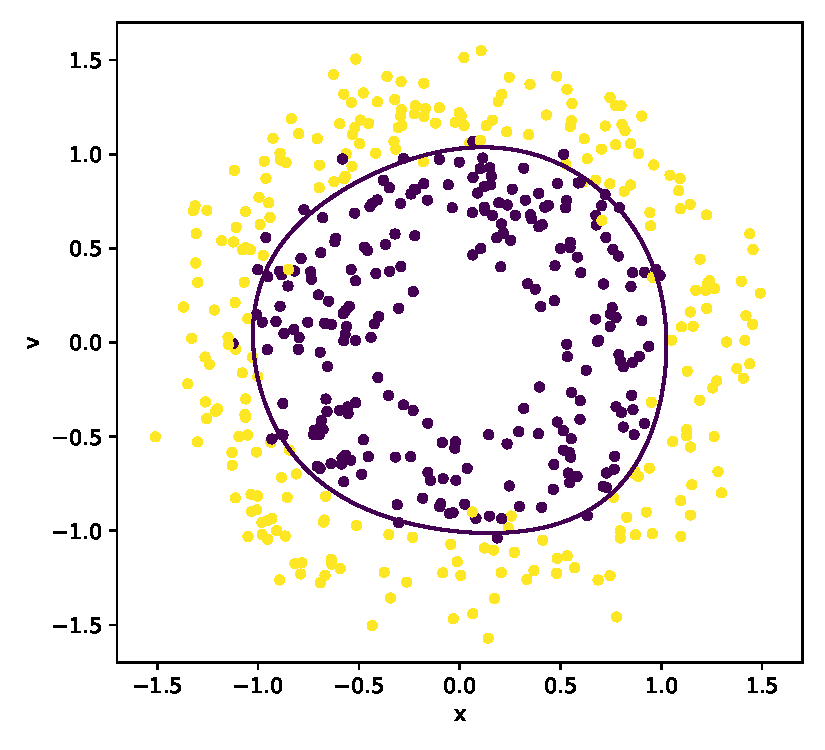
\includegraphics[width=.62\textwidth]{figures/fig_svm_phase.pdf}\caption{Kufi jolinear me SVM RBF në një hapësirë faze sintetike.}\label{fig:svm}\end{figure}
Notebook-u do të krahasojë kernel linear dhe RBF, do të eksplorojë rrjetën $(C,\gamma)$ me cross-validation dhe do të vizualizojë numrin e vektorëve mbështetës.

Për një rast linear, parametrat e hiperplanit të mësuar nga biblioteka mund të përdoren drejtpërdrejt për të vizatuar kufirin dhe dy margjinat:
\begin{lstlisting}[caption={Kufiri dhe margjinat e një SVM lineare.}]
svm = SVC(kernel="linear", C=10).fit(X, y)
w = svm.coef_[0]
b = svm.intercept_[0]

x1 = np.linspace(X[:, 0].min(), X[:, 0].max(), 200)
boundary = -(w[0] * x1 + b) / w[1]
margin_p = -(w[0] * x1 + b - 1) / w[1]
margin_m = -(w[0] * x1 + b + 1) / w[1]
\end{lstlisting}
Vizualizimi i margjinave dhe i vektorëve mbështetës është më informativ se raportimi i vetëm i saktësisë: ai tregon se cilat pika po përcaktojnë realisht vendimin.


\paragraph{Problem tipik në fizikë: dy regjime në hapësirën e fazës.}
Nëse një sistem dinamik përshkruhet nga dy veçori të nxjerra nga trajektorja, pikat mund të formojnë dy re të ndara. SVM zgjedh jo një ndarje arbitrare, por atë që maksimizon margjinën. Pikat që prekin ose afrohen me kufijtë e margjinës janë vektorët mbështetës dhe janë pikërisht ato që mbajnë informacionin vendimtar për pozicionin e hiperplanit.

\paragraph{Problem tipik jashtë fizikës: klasifikimi i dokumenteve.}
Një dokument mund të paraqitet në një hapësirë me shumë dimensione, ku secila veçori lidhet me një fjalë ose komponent tematik. Edhe pse dimensioni është i madh, një SVM linear mund të jetë shumë efikas sepse kufiri varet nga kombinimi linear i këtyre veçorive. Kernelët bëhen të dobishëm kur ndarja kërkon një gjeometri jolineare, por zgjedhja e tyre duhet validuar dhe jo bërë mekanikisht.

\begin{figure}[H]\centering
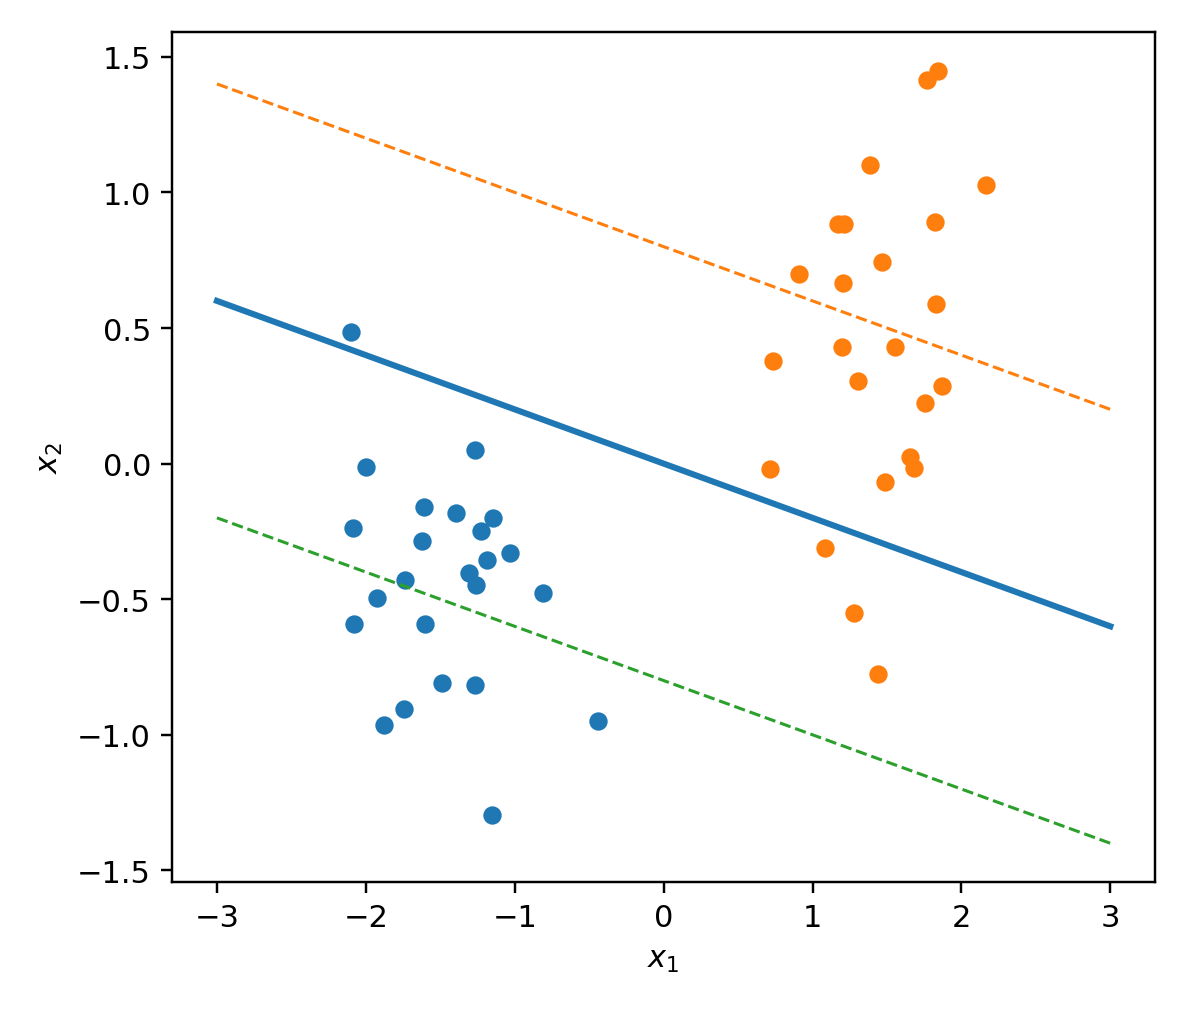
\includegraphics[width=.62\textwidth]{fig_svm_pd_adapted.png}
\caption{Hiperplani ndarës dhe margjinat në një SVM. Rivizatim i përshtatur nga \emph{SVM margins.svg}, DJGulp3, Wikimedia Commons, domen publik. \url{https://commons.wikimedia.org/wiki/File:SVM_margins.svg}.}
\end{figure}

\begin{lstlisting}
from sklearn.svm import SVC
from sklearn.pipeline import make_pipeline
from sklearn.preprocessing import StandardScaler

svm = make_pipeline(StandardScaler(),
                    SVC(C=2.0, kernel="rbf", gamma="scale"))
svm.fit(X_train, y_train)
\end{lstlisting}
Shkallëzimi është pjesë e modelit, sepse margjina dhe kerneli varen nga distancat. Për këtë arsye ai vendoset brenda tubacionit dhe jo si hap i kryer një herë mbi të gjithë bashkësinë.

\section{Ushtrime}

\textbf{1.} Tregoni pse minimizimi i $\|\mathbf w\|$ maksimizon margjinën pas normalizimit të kufizimeve. \textbf{2.} Shpjegoni rolin e $C$ me fjalë dhe me grafik. \textbf{3.} Studioni efektin e $\gamma$ në RBF. \textbf{4.} Identifikoni vektorët mbështetës dhe interpretojini fizikisht në shembullin e hapësirës së fazës. \textbf{5.} Jepni një situatë ku linear SVM është më i preferueshëm se RBF edhe nëse ky i fundit jep saktësi pak më të madhe.


\paragraph{Nga distanca gjeometrike te optimizimi konveks.}
Për një pikë $x$, distanca me hiperplanin $w^Tx+b=0$ është $|w^Tx+b|/\|w\|$. Duke shkallëzuar $w,b$ në mënyrë që pikat më të afërta të kenë $y_i(w^Tx_i+b)=1$, distanca e tyre është $1/\|w\|$ dhe gjerësia mes dy hiperplaneve mbështetëse është $2/\|w\|$. Kjo derivon objektivin $\tfrac12\|w\|^2$. SVM është prandaj shembull ku një kriter gjeometrik shndërrohet në problem optimizimi konveks.

\paragraph{Formulimi dual dhe support vectors.}
Pa zhvilluar të gjithë teorinë e shumëzuesve të Lagrange, është e vlefshme të shihet forma e vendimit
\[
f(x)=\sum_i\alpha_i y_i K(x_i,x)+b.
\]
Vetëm pikat me $\alpha_i>0$ janë support vectors. Kjo shpjegon pse modeli varet nga një nënbashkësi e të dhënave dhe pse kernel trick është i mundur: të dhënat hyjnë përmes produkteve skalare ose kernelit.

\paragraph{Roli i $C$ dhe $\gamma$.}
Në RBF SVM kemi dy shkallë kompleksiteti. $C$ vendos sa fort penalizohen shkeljet; $\gamma$ vendos sa lokale është ngjashmëria. $C$ i madh dhe $\gamma$ i madh mund të krijojnë kufij shumë të imët rreth pikave individuale. $C$ i vogël dhe $\gamma$ i vogël japin model të lëmuar dhe mund të nënpërshtatin. Harta e cross-validation në planin $(\log C,\log\gamma)$ është mënyrë e mirë për ta parë këtë ndërveprim.

\paragraph{Kerneli si zgjedhje e përfaqësimit.}
Kerneli polinomial korrespondon me ndërveprime polinomiale; RBF korrespondon me një hapësirë shumë të pasur funksionesh lokale. Në vend që ta shohim kernelin si ``magji'', duhet ta interpretojmë si mënyrë për të ndryshuar nocionin e ngjashmërisë. Në fizikë mund të ekzistojnë kernel-e të ndërtuara nga simetri ose invariante, por kjo i kalon objektivat e kursit hyrës.

\paragraph{Shembull i punuar: pika pranë tranzicionit.}
Në të dhënat e hapësirës së fazës, support vectors priren të jenë pranë kufirit midis regjimeve. Inspektimi i tyre mund të zbulojë se disa pika janë afër tranzicionit fizik, ndërsa të tjera mund të jenë outliers. Nëse heqja e pak pikave ndryshon fort kufirin, modeli është i ndjeshëm dhe duhet raportuar kjo. Support vectors janë kështu jo vetëm koncept matematik, por edhe mjet diagnostik.

\paragraph{Kur të mos përdoret SVM.}
Për miliona shembuj, kernel SVM mund të jetë e kushtueshme në memorie dhe kohë. Për interpretim të drejtpërdrejtë, një model linear ose pemë e cekët mund të jetë më e përshtatshme. Për probabilitete, SVM kërkon kalibrim shtesë. Zgjedhja e algoritmit duhet të peshojë dimensionin, madhësinë e mostrës, interpretueshmërinë dhe nevojën për probabilitete.

\chapter[PCA]{Analiza e komponentëve kryesorë (PCA)}

PCA është një nga pikat ku formimi fizik i studentit jep një avantazh të drejtpërdrejtë. Ideja e diagonalizimit të një matrice kovariance dhe e përzgjedhjes së drejtimeve kryesore është e afërt me boshtet kryesore të inercisë, modat normale dhe problemet vetjake të mekanikës kuantike. Ndryshimi është se këtu matrica përmbledh variacionin statistikor të të dhënave dhe vektorët vetjakë përcaktojnë kombinime lineare të veçorive.

Në spektroskopi, mijëra pika të një spektri mund të përmbajnë vetëm disa modele kryesore ndryshimi. Në analiza socio-ekonomike, dhjetëra tregues mund të reduktohen në disa drejtime që përmbledhin pjesën më të madhe të variacionit. PCA nuk zbulon domosdoshmërisht ``shkaqe''; ajo zbulon drejtime lineare të variacionit dhe interpretimi i tyre kërkon njohuri të problemit.
\section{Kovarianca dhe drejtimet e variacionit}

PCA nis nga një pyetje gjeometrike: në cilat drejtime ndryshojnë më shumë të dhënat? Për një fizikan, kjo është analogji e afërt me gjetjen e boshteve kryesore ose të modeve normale. Ndryshe nga klasifikimi, PCA nuk përdor etiketa; ajo përshkruan strukturën e vetë reve të pikave.

Kur çdo shembull përshkruhet nga shumë madhësi të korreluara, është e dobishme të kërkojmë drejtimet kolektive përgjatë të cilave të dhënat ndryshojnë më shumë. Pas qendrimit të kolonave, matrica e kovariancës është
\[
C=\frac{1}{N-1}X^TX.
\]
Për një drejtim njësi $\mathbf v$, varianca e projeksioneve $X\mathbf v$ është $\mathbf v^TC\mathbf v$. Maksimizimi nën kufizimin $\|\mathbf v\|=1$ çon në ekuacionin e vlerave vetjake
\[
C\mathbf v=\lambda\mathbf v.
\]
Vektori vetjak me $\lambda$ më të madhe është komponenti i parë kryesor.

\section{Derivimi variacional dhe ortogonaliteti}

Me shumëzues Lagrange, maksimizojmë $\mathbf v^TC\mathbf v-\lambda(\mathbf v^T\mathbf v-1)$. Derivimi jep $C\mathbf v=\lambda\mathbf v$. Komponenti i dytë maksimizon variancën nën kushtin shtesë të ortogonalitetit me të parin; për një matricë kovariance simetrike, vektorët vetjakë mund të zgjidhen ortonormalë.

Në praktikë PCA llogaritet shpesh me SVD të matricës së qendruar, e cila është numerikisht stabile dhe shmang formimin e $X^TX$ kur dimensioni është i madh. Vlerat singulare lidhen drejtpërdrejt me vlerat vetjake të kovariancës.

\section{Projeksioni, rindërtimi dhe varianca e shpjeguar}

Duke mbajtur $q<d$ komponentë, projektojmë
\[
Z=XV_q,
\]
ku kolonat e $V_q$ janë vektorët vetjakë të zgjedhur. Rindërtimi afërsisht është $\hat X=ZV_q^T$. PCA ka edhe një interpretim si zgjedhja e nënhapësirës lineare me dimension $q$ që minimizon gabimin kuadratik të rindërtimit.

Pjesa e variancës së shpjeguar nga komponenti $j$ është $\lambda_j/\sum_k\lambda_k$. Një grafik kumulativ ndihmon në zgjedhjen e $q$, por nuk ka prag universal. Për kompresim mund të synojmë 95--99\%; për vizualizim zgjedhim dy ose tre komponentë edhe kur humbet më shumë informacion.

\section{Shkallëzimi dhe interpretimi fizik i loadings}

Nëse veçoritë kanë njësi dhe varianca shumë të ndryshme, PCA mbi kovariancën mund të dominohet nga veçoria me shkallën më të madhe. Standardizimi përpara PCA është i arsyeshëm kur duam t'u japim veçorive peshë të krahasueshme; por nuk duhet bërë automatikisht nëse madhësia absolute e variancës ka kuptim fizik.

Koeficientët e vektorëve vetjakë quhen shpesh \emph{loadings}. Ata tregojnë si kombinohen veçoritë origjinale në komponent. Shenja e një vektori vetjak është arbitrare, ndaj interpretimi duhet të fokusohet te madhësitë relative dhe strukturat, jo te shenja absolute.

\section{Shembull: spektroskopi sintetike}

Në një spektër me 120 gjatësi vale, kolonat fqinje janë fort të korreluara. PCA mund të përmbledhë shumicën e variacionit në pak komponentë që ngjajnë me forma spektrale bazë. Figura~\ref{fig:pca} tregon variancën kumulative të shpjeguar.
\begin{figure}[H]\centering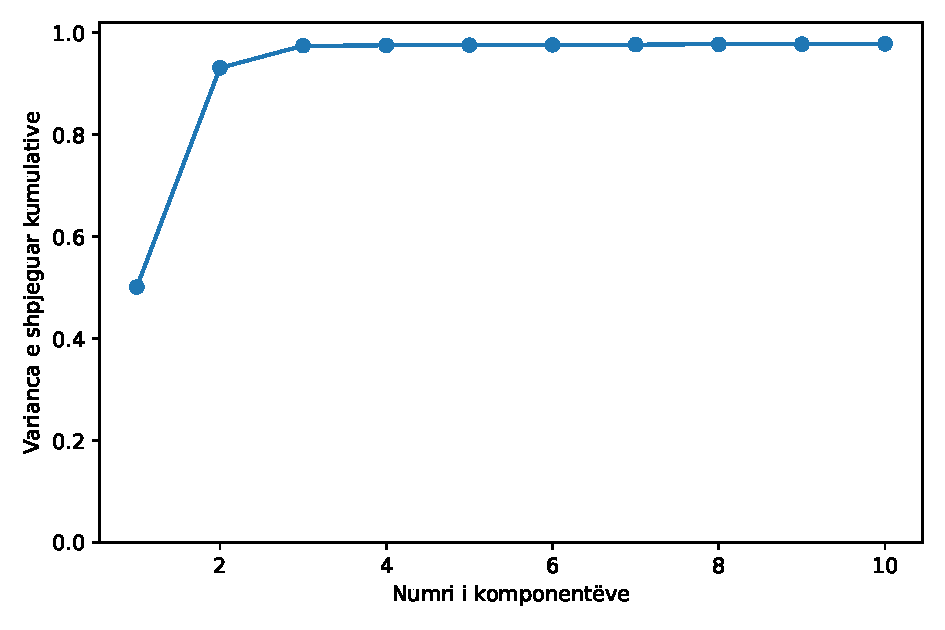
\includegraphics[width=.67\textwidth]{figures/fig_pca_variance.pdf}\caption{Varianca e shpjeguar nga PCA për spektra sintetike.}\label{fig:pca}\end{figure}
Në notebook, PCA do të ndërtohet manualisht: qendrim, kovariancë, \texttt{eigh}, renditje, projeksion. Pastaj krahasohet me \texttt{sklearn.decomposition.PCA}. Do të kontrollohet se komponentët mund të kenë shenjë të kundërt por të përfaqësojnë të njëjtin drejtim.


\paragraph{Problem tipik në fizikë: kompresimi i spektrave.}
Mendojmë $N$ spektre, secili i matur në qindra gjatësi vale. Vlerat fqinjë janë fort të korreluara dhe shumë nga dimensionet janë të tepërta. PCA ndërton kombinime lineare të pikave spektrale që kapin variacionin kryesor. Komponenti i parë mund të përfaqësojë një ndryshim të përgjithshëm të intensitetit, ndërsa komponentë të tjerë mund të lidhen me zhvendosje ose ndryshim të formës së vijave.

\paragraph{Problem tipik jashtë fizikës: përmbledhja e treguesve socio-ekonomikë.}
Një grup vendesh mund të përshkruhet nga të ardhurat, arsimi, jetëgjatësia, punësimi dhe tregues të tjerë. Shumë prej tyre janë të korreluar. PCA mund të krijojë disa drejtime që përmbledhin pjesën më të madhe të variacionit, duke ndihmuar vizualizimin. Megjithatë, emërtimi i komponentit si ``zhvillim'' ose ``mirëqenie'' është interpretim njerëzor dhe duhet justifikuar nga peshat e veçorive, jo vetëm nga grafiku.

\begin{figure}[H]\centering
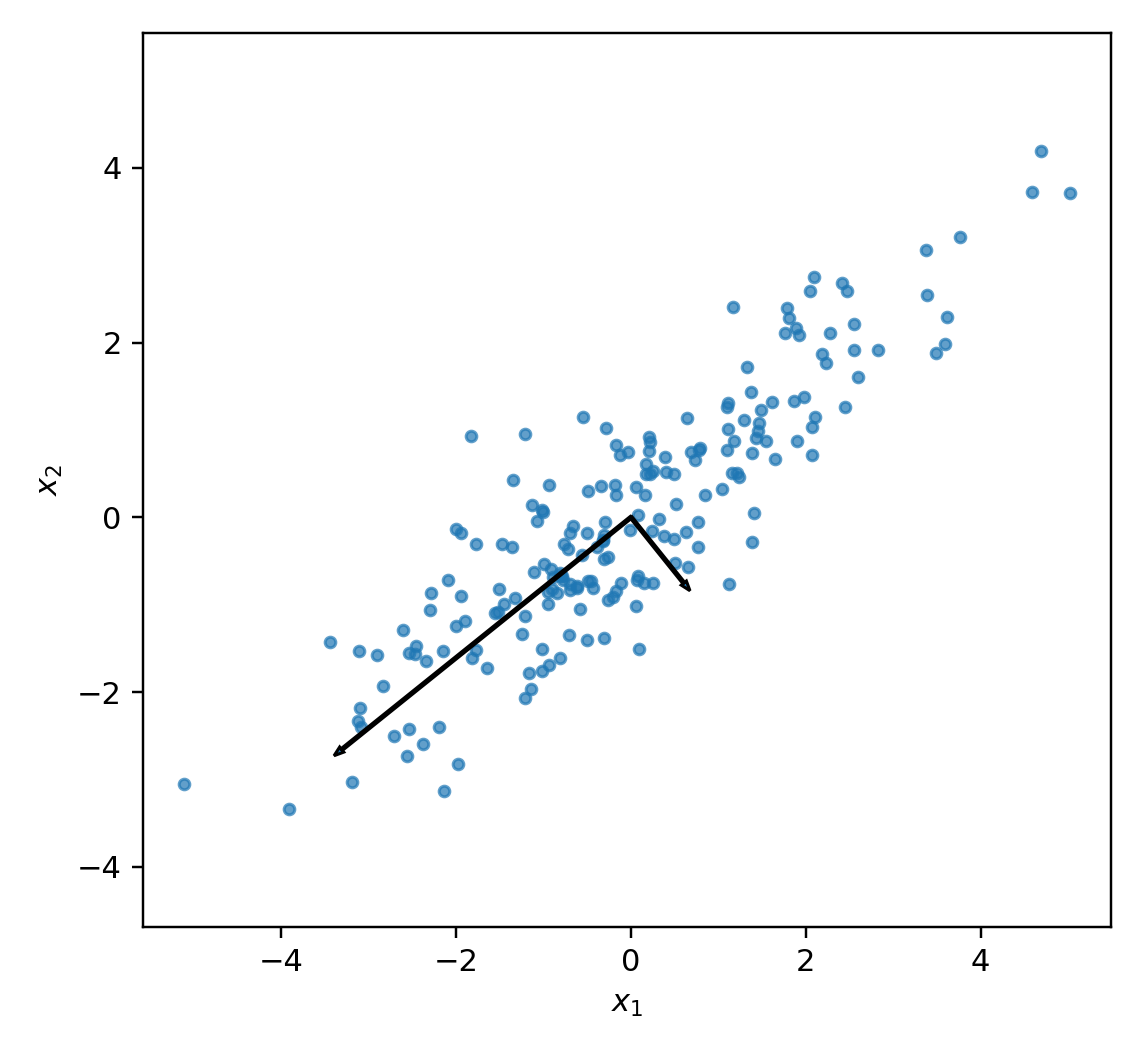
\includegraphics[width=.62\textwidth]{fig_pca_free_adapted.png}
\caption{Re pikash dhe drejtimet kryesore të variacionit. Rivizatim i përshtatur nga figura e lirë \emph{GaussianScatterPCA}, Ben FrantzDale, Wikimedia Commons, CC BY-SA 3.0/GFDL. \url{https://commons.wikimedia.org/wiki/File:GaussianScatterPCA.png}.}
\end{figure}

\begin{lstlisting}
Xc = X - X.mean(axis=0)
C = np.cov(Xc, rowvar=False)
vals, vecs = np.linalg.eigh(C)
order = np.argsort(vals)[::-1]
W = vecs[:, order[:2]]
Z = Xc @ W
\end{lstlisting}
Ky është PCA nga parimet e para: qendërzim, kovariancë, diagonalizim, renditje e vlerave vetjake dhe projeksion. Implementimi i bibliotekës duhet të japë të njëjtën nënhapësirë, deri në shenjën arbitrare të vektorëve vetjakë.

\section{Ushtrime}

\textbf{1.} Derivoni ekuacionin e vlerave vetjake nga maksimizimi i variancës. \textbf{2.} Tregoni lidhjen midis SVD dhe PCA. \textbf{3.} Krahasoni PCA me dhe pa standardizim në një bashkësi ku një veçori ka njësi shumë më të mëdha. \textbf{4.} Rindërtoni spektrat me 1, 2, 3 dhe 10 komponentë dhe matni gabimin. \textbf{5.} Shpjegoni pse PCA nuk është metodë për zbulimin e kauzalitetit.


\paragraph{PCA si problem i projeksionit optimal.}
Për një komponent, kërkojmë një vektor njësi $v$ që maksimizon variancën $\|Xv\|^2/(N-1)$. Me shumëzues Lagrange marrim $Cv=\lambda v$. Për $q$ komponentë, zgjidhja optimale është nënhapësira e gjeneruar nga $q$ vektorët vetjakë me vlerat më të mëdha. E njëjta nënhapësirë minimizon shumën e katrorëve të distancave të pikave nga rindërtimi. Kjo dualitet midis ``maksimizimit të variancës'' dhe ``minimizimit të gabimit të rindërtimit'' është një nga arsyet pse PCA është kaq qendrore.

\paragraph{PCA dhe SVD.}
Nëse $X_c=U\Sigma V^T$, kolonat e $V$ janë drejtimet kryesore, ndërsa $\lambda_j=\sigma_j^2/(N-1)$. Koordinatat kryesore janë $U\Sigma=X_cV$. Ky formulim është praktik sepse bibliotekat numerike kanë implementime shumë të qëndrueshme të SVD dhe mund të trajtojnë edhe raste kur numri i veçorive është më i madh se numri i shembujve.

Një implementim nga parimet e para mund të bëhet drejtpërdrejt përmes matricës së kovariancës:
\begin{lstlisting}[caption={PCA nga kovarianca dhe dekompozimi në vlera vetjake.}]
Xc = X - X.mean(axis=0)
C = np.cov(Xc, rowvar=False)
values, vectors = np.linalg.eigh(C)
order = np.argsort(values)[::-1]
values = values[order]
vectors = vectors[:, order]
explained = values / values.sum()
Z = Xc @ vectors[:, :2]
\end{lstlisting}
Vektorët vetjakë japin drejtimet kryesore, ndërsa raporti \texttt{explained} tregon sa nga varianca totale mbart secila prej tyre. Në një spektër fizik, ngarkesat e komponentëve duhet të interpretohen si modele ndryshimi në gjatësi vale, jo si ``veçori të reja'' pa kuptim.

\paragraph{Qendrimi kundrejt standardizimit.}
Qendrimi është pjesë thelbësore e PCA standarde: pa të, komponenti i parë mund të ndjekë thjesht vektorin e mesatares. Standardizimi është vendim shtesë. Në spektra ku të gjitha kolonat kanë të njëjtën njësi dhe amplituda e variacionit është fizikisht informative, standardizimi i çdo gjatësi vale në variancë njësi mund të shtrembërojë pyetjen. Në të dhëna ku kolonat janë temperaturë, presion dhe shpejtësi ere me njësi të ndryshme, standardizimi mund të jetë i domosdoshëm.

\paragraph{Loadings dhe komponentët si modele fizike.}
Në spektroskopi, loading i parë mund të përfaqësojë ndryshim të përgjithshëm të intensitetit, i dyti një zhvendosje të pikut dhe i treti një ndryshim të gjerësisë. Por PCA nuk garanton që komponentët korrespondojnë me mekanizma të pavarur fizikë; ata janë drejtime ortogonale statistikore. Nëse mekanizmat fizikë nuk janë ortogonalë në hapësirën e matjeve, PCA mund t'i përziejë.

\paragraph{Shembull i punuar: kompresimi.}
Nëse 120 kanale spektrale kompresohen në 3 komponentë dhe këta shpjegojnë 98\% të variancës, raporti bruto i dimensionit është 40:1 për çdo spektër, por duhet të ruajmë edhe mesataren dhe tre vektorët loading. Për një numër të madh spektrash kjo kosto është e vogël. Gabimi i rindërtimit duhet të krahasohet me zhurmën instrumentale: nëse është më i vogël se zhurma, kompresimi ka humbur pak informacion të matshëm.

\paragraph{PCA para klasifikimit.}
PCA është e pambikëqyrur dhe nuk përdor etiketat. Drejtimi me variancë të madhe nuk është domosdoshmërisht drejtimi që ndan klasat. Prandaj PCA mund të heqë informacion diskriminues me variancë të vogël. Kur përdoret para klasifikimit, numri i komponentëve duhet të jetë hiperparametër i pipeline-it dhe të zgjidhet brenda cross-validation. Ky shembull përforcon parimin e rrjedhjes së informacionit dhe tregon pse preprocessing nuk mund të ndahet nga modeli.

\chapter[Grupimi]{Grupimi i të dhënave}

Grupimi është një nga detyrat ku duhet të jemi më të kujdesshëm me gjuhën. Algoritmi mund të gjejë grupe sipas një distance të caktuar, por kjo nuk do të thotë automatikisht se këto grupe përfaqësojnë faza fizike, kategori biologjike ose segmente sociale reale. Kuptimi i grupimit lind vetëm kur struktura numerike përputhet me një argument të pavarur shkencor ose praktik.

Në meteorologji, ditët mund të grupohen sipas temperaturës, lagështisë, presionit dhe erës për të identifikuar regjime atmosferike. Në tregti, klientët mund të grupohen sipas shpeshtësisë së blerjeve, vlerës mesatare dhe kategorive të produkteve. Në të dyja rastet, shkallëzimi i veçorive dhe zgjedhja e numrit të grupeve mund të ndryshojnë përfundimin në mënyrë thelbësore.
\section{Problemi i pambikëqyrur}

Në \term{nxënien e pambikëqyrur}{unsupervised learning} nuk ekziston etiketë që të thotë nëse rezultati është ``i saktë''. Struktura që zbulojmë varet nga përkufizimi i ngjashmërisë dhe nga algoritmi. Kjo kërkon kujdes të veçantë në interpretim: një grup numerik nuk është automatikisht një fazë fizike.

k-means kërkon ndarje në $K$ grupe që minimizon
\[
J=\sum_{k=1}^K\sum_{\mathbf x_i\in C_k}\|\mathbf x_i-\boldsymbol\mu_k\|^2,
\]

\paragraph{Interpretim.}
Objektivi $J$ favorizon grupe kompakte rreth qendrave të tyre. Ai nuk mat ``realitetin'' e një faze fizike; mat vetëm një nocion të caktuar të kompaktësisë Euklidiane. Prandaj k-means ka prirje të funksionojë mirë për grupe afërsisht sferike dhe me shkallë të krahasueshme, ndërsa mund të jetë i papërshtatshëm për struktura të zgjatura ose me dendësi shumë të ndryshme.
ku $\boldsymbol\mu_k$ është qendra e grupit. Algoritmi alternon midis caktimit të çdo pike te qendra më e afërt dhe përditësimit të qendrave si mesatare e pikave të caktuara.

Kjo alternim mund të shihet drejtpërdrejt në një implementim të thjeshtë:
\begin{lstlisting}[caption={Hapat bazë të k-means.}]
for _ in range(max_iter):
    d2 = ((X[:, None, :] - centers[None, :, :])**2).sum(axis=2)
    labels = d2.argmin(axis=1)
    new_centers = np.vstack([
        X[labels == k].mean(axis=0) for k in range(K)
    ])
    if np.allclose(new_centers, centers):
        break
    centers = new_centers
\end{lstlisting}
Çdo iteracion nuk e rrit $J$, por algoritmi mund të përfundojë në minimum lokal. Kjo është arsyeja pse inicializimi dhe përsëritjet me fara të ndryshme janë pjesë e metodës, jo detaje dytësore.

\section{Konvergjenca, inicializimi dhe minimumet lokale}

Çdo hap i k-means nuk e rrit funksionin objektiv, prandaj procedura konvergon në një zgjidhje lokale pas një numri të fundëm konfigurimesh. Por rezultati varet nga inicializimi. k-means++ zgjedh qendrat fillestare në mënyrë që ato të jenë të shpërndara dhe zakonisht jep zgjidhje më të mira se zgjedhja plotësisht e rastësishme.

Për një analizë serioze përdoren disa nisje dhe studiohet stabiliteti. Nëse ndarja ndryshon fort nga një nisje te tjetra, struktura e pretenduar është e dobët ose kriteri Euklidian nuk është i përshtatshëm.

\section{Zgjedhja e numrit të grupeve}

Inercia $J$ bie gjithmonë kur $K$ rritet, ndaj nuk mund të zgjedhim $K$ duke minimizuar thjesht $J$. Metoda e bërrylit kërkon pikën ku përfitimi marginal zvogëlohet, por është subjektive. \term{Silhouette score} krahason kohezionin brenda grupit me distancën ndaj grupit më të afërt dhe varion afërsisht nga $-1$ në 1.

Asnjë kriter nuk zëvendëson interpretimin fizik. Nëse një analizë atmosferike jep tre grupe, duhet të kontrollojmë nëse ato lidhen me regjime të njohura, stinët, pozicionin gjeografik ose ndonjë artefakt të instrumentit.

\section{Grupimi hierarkik}

Grupimi hierarkik aglomerativ fillon me çdo pikë si grup më vete dhe bashkon gradualisht grupet sipas një rregulli lidhjeje. Single linkage përdor distancën minimale, complete linkage maksimalen, average linkage mesataren, ndërsa Ward minimizon rritjen e variancës brenda grupeve.

\term{Dendrograma}{dendrogram} paraqet historinë e bashkimeve dhe e bën të dukshme strukturën në disa shkallë. Kjo është përparësi ndaj k-means kur nuk duam të zgjedhim menjëherë një $K$ të vetëm. Megjithatë, kompleksiteti llogaritës rritet shpejt me numrin e pikave.

\section{Shembull: regjime atmosferike}

Të dhënat sintetike për temperaturën, lagështinë relative dhe presionin përmbajnë tre regjime të fshehta. Figura~\ref{fig:kmeans} tregon projeksionin temperaturë--lagështi të grupeve të gjetura. Standardizimi është i domosdoshëm sepse presioni ka shkallë numerike shumë më të madhe.
\begin{figure}[H]\centering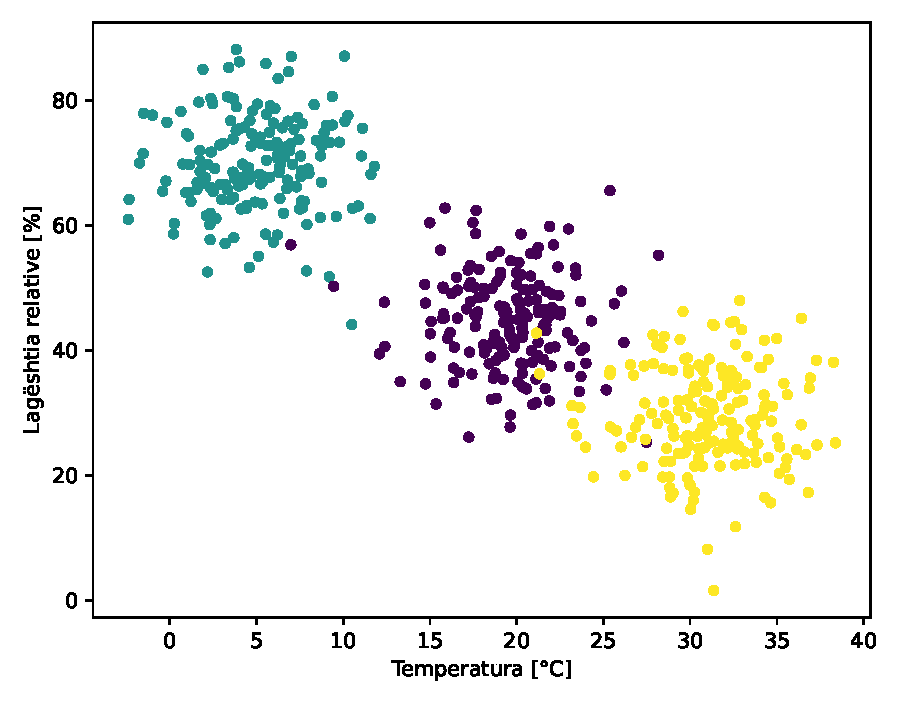
\includegraphics[width=.67\textwidth]{figures/fig_kmeans_atmosfera.pdf}\caption{Grupim k-means i regjimeve atmosferike sintetike.}\label{fig:kmeans}\end{figure}
Notebook-u do të implementojë k-means nga e para, do të paraqesë trajektoren e qendrave dhe do të krahasojë disa inicializime. Pastaj do të ndërtojë dendrogramë dhe do të diskutojë raste ku grupet janë jo sferike dhe k-means dështon.


\paragraph{Problem tipik në fizikë: regjime atmosferike.}
Çdo ditë mund të përshkruhet nga temperatura, presioni, lagështia, era dhe një ose dy tregues të stabilitetit. Në mungesë të etiketave, $k$-means mund të propozojë grupe të ditëve me karakteristika të ngjashme. Këto grupe nuk duhet të quhen menjëherë ``regjime meteorologjike''; ato bëhen fizikisht kuptimplota vetëm pasi kontrollohen ndaj hartave sinoptike, stinëve dhe variablave të pavarura.

\paragraph{Problem tipik jashtë fizikës: segmentimi i klientëve.}
Një biznes mund të përmbledhë sjelljen e klientëve me numrin e blerjeve, shpenzimin mesatar dhe kohën nga blerja e fundit. Grupimi propozon segmente me sjellje të ngjashme. Rezultati varet shumë nga shkalla e variablave dhe nga zgjedhja e $k$; për këtë arsye silhouette score dhe analiza e stabilitetit janë ndihmë, jo zëvendësim për arsyetimin e domenit.

\begin{figure}[H]\centering
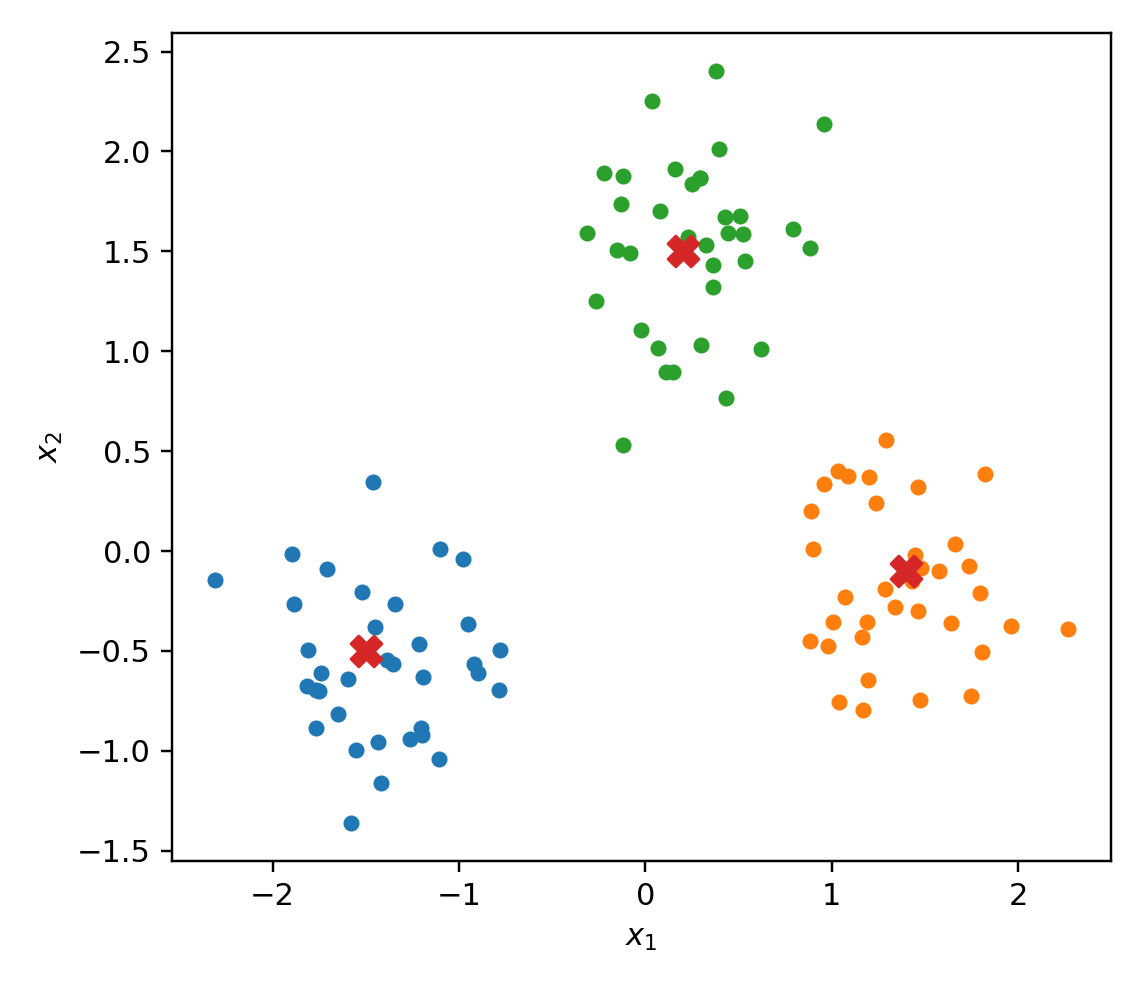
\includegraphics[width=.62\textwidth]{fig_kmeans_free_adapted.png}
\caption{Parimi i $k$-means: pikat caktohen te qendra më e afërt dhe qendrat ripërllogariten. Rivizatim i përshtatur nga seria \emph{K Means Example}, Weston.pace, Wikimedia Commons (licencë e lirë GFDL/CC sipas faqes së skedarit). \url{https://commons.wikimedia.org/wiki/File:K_Means_Example_Step_1.svg}.}
\end{figure}

\begin{lstlisting}
for _ in range(max_iter):
    d2 = ((X[:, None, :] - centroids[None, :, :])**2).sum(axis=2)
    labels = d2.argmin(axis=1)
    new = np.vstack([X[labels == j].mean(axis=0) for j in range(k)])
    if np.allclose(new, centroids):
        break
    centroids = new
\end{lstlisting}
Kodi e bën të dukshme natyrën alternative të algoritmit: hapi i caktimit dhe hapi i përditësimit përsëriten derisa qendrat të stabilizohen.

\section{Ushtrime}

\textbf{1.} Tregoni se qendra që minimizon shumën e distancave kuadratike brenda një grupi është mesatarja. \textbf{2.} Implementoni një iteracion të plotë të k-means. \textbf{3.} Studioni efektin e mosstandardizimit të presionit. \textbf{4.} Krahasoni Ward dhe single linkage. \textbf{5.} Ndërtoni një shembull me dy gjysmëhëna ku k-means është konceptualisht i papërshtatshëm.


\paragraph{Çfarë do të thotë një cluster?}
Një cluster nuk është objekt i pavarur nga algoritmi. k-means kërkon grupe kompakte rreth centroidëve sipas distancës Euklidiane. Hierarchical clustering mund të prodhojë struktura të tjera sipas linkage. DBSCAN, që përmendet vetëm si perspektivë, kërkon rajone me densitet. Në të njëjtat të dhëna këto metoda mund të japin ndarje të ndryshme, secila e vlefshme sipas kriterit të vet.

Në fizikë duhet të shmanget rrëshqitja nga ``algoritmi gjeti tre grupe'' te ``ekzistojnë tre faza fizike''. Për të bërë pretendimin e dytë duhen kontrolle të jashtme: varësi nga temperatura, përputhje me teori, reproducibility në eksperimente të pavarura ose ndryshime të madhësive të tjera fizike.

\paragraph{Derivimi i centroidit.}
Për një grup fiks $C$, minimizojmë $\sum_{i\in C}\|x_i-\mu\|^2$. Derivimi sipas $\mu$ jep $-2\sum_i(x_i-\mu)=0$, prandaj $\mu$ është mesatarja. Ky rezultat shpjegon hapin e përditësimit të k-means dhe tregon pse algoritmi është i lidhur me humbjen kuadratike. Nëse përdorim distancën $L_1$, qendra optimale nuk është mesatarja por mediana komponent për komponent; kështu zgjedhja e metrikes ndryshon edhe përfaqësuesin natyror të cluster-it.

\paragraph{Stabiliteti si kriter.}
Përveç silhouette, mund të studiojmë sa të qëndrueshme janë grupet ndaj rimostrimit, zhurmës ose ndryshimit të inicializimit. Nëse të njëjtat pika kalojnë shpesh nga një cluster në tjetrin, kufiri midis grupeve është i pasigurt. Për analiza shkencore është e dobishme të raportohen këto zona të paqarta, jo vetëm një etiketë e fortë për çdo pikë.

\paragraph{Hierarkia dhe shkallët.}
Dendrograma nuk ka vetëm një prerje ``të saktë''. Në një lartësi mund të shohim dy makro-regjime, në një tjetër katër nënregjime. Kjo është veçanërisht e përshtatshme për sisteme ku struktura fizike është hierarkike, si klasifikime astronomike ose regjime meteorologjike. Linkage i ndryshëm mund të ndryshojë pemën dhe duhet interpretuar në lidhje me gjeometrinë e të dhënave.

\paragraph{Shembull i punuar: një veçori dominante.}
Në dataset-in atmosferik presioni është rreth 1000 hPa, temperatura rreth dhjetëra gradë dhe lagështia 0--100. Pa standardizim, ndryshimet e presionit mund të dominojnë distancën edhe nëse relativisht janë të vogla. Pas standardizimit, secila veçori kontribuon në njësi të devijimit standard. Por ky transformim supozon se një devijim standard temperature dhe një devijim standard presioni kanë peshë të krahasueshme për pyetjen tonë. Ky është supozim metodologjik, jo e vërtetë universale.

\paragraph{Kufijtë e k-means.}
Grupet jo-konvekse, madhësi shumë të ndryshme ose densitete të ndryshme mund të dështojnë. Shembulli i dy gjysmëhënave e bën këtë të dukshme: centroidët e ndajnë hapësirën në rajone Voronoi dhe nuk mund të ndjekin formën e lakuar. Studentët duhet të mësojnë të njohin dështimin e modelit, jo të kërkojnë vetëm një konfigurim që jep një figurë të bukur.

\chapter[Modelet dhe pasiguria]{Krahasimi i modeleve dhe pasiguria}

Një kurs i mirë i nxënies automatike nuk duhet të përfundojë me pyetjen ``cili algoritëm dha saktësinë më të lartë?''. Pyetja shkencore është më e gjerë: sa i qëndrueshëm është rezultati, si ndryshon nga një ndarje e të dhënave në tjetrën, sa varet nga hiperparametrat, a është i kalibruar dhe a mbetet i besueshëm kur të dhënat ndryshojnë pak? Këtu krahasimi i modeleve bëhet pjesë e metodologjisë së eksperimentit.

Në fizikën eksperimentale, një përmirësim shumë i vogël i saktësisë mund të mos justifikojë një model shumë më të ndërlikuar nëse ai është i paqëndrueshëm ose i vështirë për t'u interpretuar. Në një proces industrial apo financiar, një model pak më pak i saktë mund të jetë i preferueshëm nëse reagimi i tij ndaj të dhënave jashtë shpërndarjes së trajnimit është më i kontrolluar. Kjo është arsyeja pse pasiguria dhe robustësia duhet të lexohen bashkë me metrikat mesatare.
\section{Një eksperiment i drejtë krahasimi}

Krahasimi i modeleve është vetë një eksperiment numerik. Për të qenë i drejtë, modelet duhet të shohin të njëjtat ndarje të të dhënave, të njëjtat veçori të disponueshme dhe të njëjtën procedurë vlerësimi. Përndryshe diferenca e raportuar mund të vijë nga protokolli, jo nga algoritmi.

Krahasimi i algoritmeve ka kuptim vetëm kur procedura është e njëjtë për të gjithë. Duhet të përdoren të njëjtat ndarje, të njëjtat metrika dhe preprocessing i përshtatur brenda çdo fold-i. Nëse SVM standardizohet por k-NN jo, nuk po krahasojmë algoritmet, por dy pipeline me cilësi metodologjike të ndryshme.

Një \term{model bazë}{baseline} i thjeshtë është i domosdoshëm. Për klasifikim mund të jetë parashikimi i klasës më të shpeshtë ose regresioni logjistik. Një metodë komplekse duhet të justifikojë kompleksitetin me përmirësim të qëndrueshëm, jo me një fitore të vogël në një ndarje të vetme.

\section{Variabiliteti i performancës dhe bootstrap}

Një numër i vetëm si accuracy=0.91 fsheh pasigurinë. Rezultatet e cross-validation japin një shpërndarje të performancës ndaj ndarjeve. Diferenca 0.910 kundrejt 0.905 mund të jetë e parëndësishme nëse devijimi midis fold-eve është 0.02.

\term{Bootstrap}{bootstrap} rimostron me zëvendësim nga të dhënat dhe lejon vlerësimin empirik të shpërndarjes së koeficientëve, metrikave ose parashikimeve. Ai është mjet fleksibël, por duhet të respektojë strukturën e të dhënave; për seri kohore ose grupe të korreluara, bootstrap i pavarur i rreshtave mund të jetë i gabuar.

Në notebook, krahasimi bëhet me të njëjtat fold-e për çdo model. Kjo lejon që rezultatet fold-pas-fold-i të krahasohen si çifte dhe jo si numra të izoluar:
\begin{lstlisting}[caption={Krahasim i disa modeleve me të njëjtën skemë validimi.}]
models = {
    "LogReg": make_pipeline(StandardScaler(), LogisticRegression()),
    "kNN": make_pipeline(StandardScaler(), KNeighborsClassifier(11)),
    "Tree": DecisionTreeClassifier(max_depth=5, random_state=0),
    "RF": RandomForestClassifier(n_estimators=250, random_state=0),
    "SVM": make_pipeline(StandardScaler(), SVC(C=3))
}

for name, model in models.items():
    scores = cross_val_score(model, X, y, cv=cv, scoring="roc_auc")
    print(name, scores.mean(), scores.std())
\end{lstlisting}
Mesatarja përmbledh performancën tipike, ndërsa shpërndarja tregon sa e ndjeshme është ajo ndaj mostrës. Një avantazh shumë i vogël në mesatare mund të mos ketë rëndësi praktike nëse variabiliteti është i madh.

\section{Pasiguria aleatorike dhe epistemike}

\term{Pasiguria aleatorike}{aleatoric uncertainty} buron nga rastësia e procesit dhe zhurma e matjes. Edhe modeli perfekt nuk mund ta eliminojë. \term{Pasiguria epistemike}{epistemic uncertainty} lidhet me mungesën e njohurive, të dhënave ose modelit adekuat. Kjo e fundit mund të zvogëlohet me matje të reja informative.

Në këtë kurs nuk ndërtojmë një teori të plotë probabilistike të pasigurisë. Synimi është që studentët të mos barazojnë parashikimin me të vërtetën. Në regresion përdorim rezidualet, intervalet e koeficientëve dhe bootstrap; në klasifikim studiojmë variabilitetin e metrikave, kalibrimin dhe stabilitetin ndaj perturbimeve.

\section{Interpretueshmëria pa pretendime të tepërta}

Modelet lineare japin koeficientë, pemët japin rregulla, random forest mund të analizojë permutation importance, PCA jep loadings dhe SVM identifikon vektorë mbështetës. Këto janë dritare mbi sjelljen e modelit. Ato nuk provojnë kauzalitet.

Një kontroll i fuqishëm në fizikë është \emph{plausibiliteti}: nëse modeli pretendon se një veçori zhurme është më e rëndësishme se energjia e matur, duhet hetuar. Mund të ketë rrjedhje informacioni, bias të përzgjedhjes ose korrelacion instrumental. Interpretueshmëria është proces diagnostik, jo dekorim pas trajnimit.

\section{Shembull i integruar i krahasimit}

Në bashkësinë e kursit për ngjarje detektori krahasohen regresioni logjistik, k-NN, pema, random forest dhe SVM. Vlerësohen accuracy dhe ROC-AUC, por edhe koha e trajnimit, stabiliteti i fold-eve, ndjeshmëria ndaj shkallëzimit dhe ndaj zhurmës. Një veçori zhurme është futur qëllimisht për të studiuar interpretimin e rëndësisë së veçorive.

Qëllimi nuk është të shpallet një ``kampion''. Nëse random forest fiton me 0.5 pikë përqindjeje por regresioni logjistik është shumë më i interpretuar dhe më stabil, zgjedhja mund të varet nga përdorimi. Në një analizë shkencore, transparenca dhe kontrolli sistematik mund të vlejnë më shumë se përmirësimi minimal i një metrike.


\paragraph{Problem tipik në fizikë: zgjedhja e klasifikuesit për një detektor.}
Supozoni se pesë modele japin saktësi të ngjashme për ndarjen sinjal--sfond. Një pyll i rastësishëm mund të fitojë me pak përqindje, por një regresion logjistik mund të jetë më i kalibruar dhe më i lehtë për t'u kontrolluar. Një SVM mund të jetë më i qëndrueshëm ndaj një kufiri të caktuar, por më i vështirë për interpretim. Vendimi shkencor kërkon të shohim shpërndarjen e rezultateve në validim, jo vetëm një numër të vetëm.

\paragraph{Problem tipik jashtë fizikës: parashikimi i largimit të klientëve.}
Në një kompani shërbimesh, një model mund të parashikojë cilët klientë kanë gjasa të largohen. Një model me AUC pak më të lartë mund të jetë më pak i dobishëm nëse probabilitetet e tij janë të pakalibruara ose nëse performanca ndryshon shumë nga një segment i popullsisë te tjetri. Këtu pasiguria, kalibrimi dhe interpretimi lidhen drejtpërdrejt me vendimin operacional.

\begin{lstlisting}
from sklearn.model_selection import StratifiedKFold, cross_validate
cv = StratifiedKFold(5, shuffle=True, random_state=7)
result = cross_validate(model, X, y, cv=cv,
                        scoring=["accuracy", "f1", "roc_auc"],
                        return_train_score=True)
\end{lstlisting}
Tabela që del nga ky eksperiment duhet lexuar si një shpërndarje performancash. Mesatarja pa devijimin standard humbet një pjesë të rëndësishme të informacionit mbi stabilitetin e modelit.

\section{Protokoll për një projekt të riprodhueshëm}

Një projekt i mirë dokumenton: pyetjen shkencore; origjinën dhe njësitë e të dhënave; kriteret e përjashtimit; ndarjen e të dhënave; baseline; pipeline; hapësirën e hiperparametrave; metrikat; analizën e pasigurisë; kontrollet e robustësisë dhe kufijtë e vlefshmërisë. Rezultati final duhet të mund të riprodhohet nga një mjedis i specifikuar dhe fara të dokumentuara.

\textbf{Ushtrime.} (i) Krahasoni pesë modele me të njëjtat split-e. (ii) Kryeni bootstrap të AUC dhe raportoni intervalin 95\%. (iii) Shtoni zhurmë në çdo veçori dhe matni degradimin. (iv) Krahasoni feature importance me permutation importance. (v) Shkruani një paragraf ku argumentoni zgjedhjen e modelit pa përdorur vetëm fjalinë ``ka saktësinë më të lartë''.


\paragraph{Krahasimi si problem inferencial.}
Kur dy modele kanë mesatare cross-validation të afërta, nuk mjafton të renditen sipas shifrës së tretë dhjetore. Fold-et përdorin të njëjtat të dhëna dhe rezultatet janë të çiftuara. Diferencat fold-pas-fold-i japin informacion më të mirë se dy devijime standarde të raportuara veçmas. Për një kurs hyrës mjafton të vizatohen diferencat dhe intervalet bootstrap; testet statistikore formale për krahasimin e klasifikuesve mund të studiohen më vonë.

\paragraph{Nested cross-validation.}
Në cross-validation të zakonshëm, nëse përdorim të njëjtat fold-e për të zgjedhur hiperparametrin dhe për të raportuar performancën, vlerësimi mund të jetë optimist. Nested CV përdor një cikël të brendshëm për tuning dhe një cikël të jashtëm për vlerësim. Kjo është metodë e fuqishme kur dataset-i është i vogël dhe nuk duam të rezervojmë test të madh. Kostoja është llogaritëse dhe konceptuale, prandaj në kurs përdoret kryesisht si material i zgjeruar.

\paragraph{Domain shift dhe robustësia.}
Cross-validation supozon se trajnimi dhe përdorimi vijnë nga i njëjti shpërndarje. Në praktikë sensori plaket, klima ndryshon, aparatura kalibrohet ndryshe ose kampioni i ardhshëm ka përbërje të re. Një test robustësie mund të perturbjë veçoritë brenda pasigurive matëse, të ndryshojë prevalencën e klasave ose të vlerësojë modelin në një grup të mbajtur sipas kohës. Këto eksperimente janë shpesh më informative se një grid search shumë i gjerë.

\paragraph{Pasiguria e parashikimit.}
Për modelet lineare mund të llogariten intervale analitike në kushte të caktuara. Për modele të përgjithshme, bootstrap mund të përdoret për të trajnuar shumë kopje të modelit në rimostrime dhe për të parë shpërndarjen e parashikimit. Ky nuk është zëvendësim për një model probabilistik të plotë, por i mëson studentit se parashikimi ka variabilitet.

\paragraph{Interpretueshmëria dhe kontrollet negative.}
Një veçori zhurme e futur qëllimisht është kontroll negativ. Një model që i jep asaj rëndësi të lartë mund të jetë duke mbipërshtatur ose importance mund të jetë e paqëndrueshme. Në projekte reale mund të përdoren veçori që dihet se nuk duhet të kenë lidhje fizike për të testuar pipeline-in. Kjo qasje është e afërt me kontrollet negative në eksperiment dhe i jep ML një kulturë më shkencore.

\paragraph{Struktura e raportit final.}
Një raport i mirë nuk fillon me ``përdorëm Random Forest''. Ai fillon me pyetjen, dataset-in dhe kriterin e suksesit. Pastaj jep baseline, procedurën e validimit, modelet kandidate, tuning, performancën me pasiguri, interpretimin dhe kufijtë. Figura duhet të përgjigjet një pyetjeje: learning curve për sasinë e të dhënave; validation curve për hiperparametrin; residual plot për modelin e gabimit; calibration curve për probabilitetet. Kjo strukturë do të përdoret edhe në projektet e kursit.

\chapter[Optimizimi me gradient]{Zbritja e gradientit dhe optimizimi}

Zbritja e gradientit lidh drejtpërdrejt nxënien automatike me metodat numerike. Në vend që të kemi një zgjidhje të mbyllur, ndërtojmë një varg të përafërt zgjidhjesh dhe përdorim informacionin lokal të gradientit për të ulur funksionin objektiv. Sjellja e algoritmit varet jo vetëm nga forma e funksionit, por edhe nga shkallëzimi i koordinatave, kondicionimi dhe zgjedhja e hapit.

Në një problem fizik kjo mund të nënkuptojë përshtatjen iteruese të parametrave të një modeli jo linear ndaj matjeve. Në një problem ekonomik ose të marketingut, e njëjta procedurë mund të minimizojë humbjen e një modeli që parashikon kërkesën ose probabilitetin e një reagimi. Pavarësisht aplikimit, analiza e konvergjencës dhe diagnostika numerike janë pjesë e problemit, jo detaje implementimi.
\section{Optimizimi si problem i përgjithshëm}

Shumë metoda të nxënies automatike përcaktojnë parametrat duke minimizuar një funksion humbjeje. Kur nuk kemi zgjidhje të mbyllur ose kur të dhënat janë shumë të mëdha, përdorim optimizim iterativ. \term{Zbritja e gradientit}{gradient descent} përditëson
\[
\boldsymbol\theta_{n+1}=\boldsymbol\theta_n-\eta\nabla \mathcal L(\boldsymbol\theta_n),
\]

\paragraph{Interpretim.}
Gradienti tregon drejtimin e rritjes më të shpejtë lokale të funksionit të humbjes; shenja minus zgjedh drejtimin e kundërt. Parametri $\eta$ përcakton gjatësinë e hapit dhe është po aq i rëndësishëm sa drejtimi. Një gradient i saktë me hap tepër të madh mund të divergojë, ndërsa hap tepër i vogël e bën algoritmin praktikisht të ngadaltë.
ku $\eta$ është \term{shpejtësia e të nxënit}{learning rate}.

Gradienti jep drejtimin e rritjes më të shpejtë lokale; shenja minus lëviz në drejtimin e uljes. Ky është pohim lokal. Në funksione konvekse, kushtet janë të favorshme dhe minimumi global mund të arrihet; në funksione jokonvekse sjellja është më komplekse.

\section{Shembull kuadratik dhe konvergjenca}

Për $\mathcal L(\theta)=\theta^2$, përditësimi është $\theta_{n+1}=(1-2\eta)\theta_n$. Konvergjenca kërkon $|1-2\eta|<1$, pra $0<\eta<1$. Ky shembull i thjeshtë tregon se hap shumë i madh mund të shkaktojë oscilacione ose divergjencë, ndërsa hap shumë i vogël jep konvergjencë të ngadaltë.

Eksperimenti numerik më poshtë e bën këtë kusht të dukshëm pa teori shtesë:
\begin{lstlisting}[caption={Ndikimi i shpejtësisë së të nxënit në një problem kuadratik.}]
def grad(theta):
    return 2.0 * theta

for eta in [0.01, 0.1, 0.8, 1.1]:
    theta = 4.0
    history = [theta]
    for _ in range(25):
        theta -= eta * grad(theta)
        history.append(theta)
    plt.plot(history, label=f"eta={eta}")
\end{lstlisting}
Për $\eta=1.1$ amplituda rritet dhe iteracioni divergon; për vlera të ndërmjetme mund të ketë oscilacione që zbehen. Grafiku i trajektores së optimizimit është prandaj një mjet diagnostik, jo vetëm ilustrim grafik.

Figura~\ref{fig:gd} paraqet tre shpejtësi të nxënit. Qëllimi nuk është të memorizohet një vlerë optimale, por të kuptohet marrëdhënia midis lakimit të funksionit dhe madhësisë së hapit.
\begin{figure}[H]\centering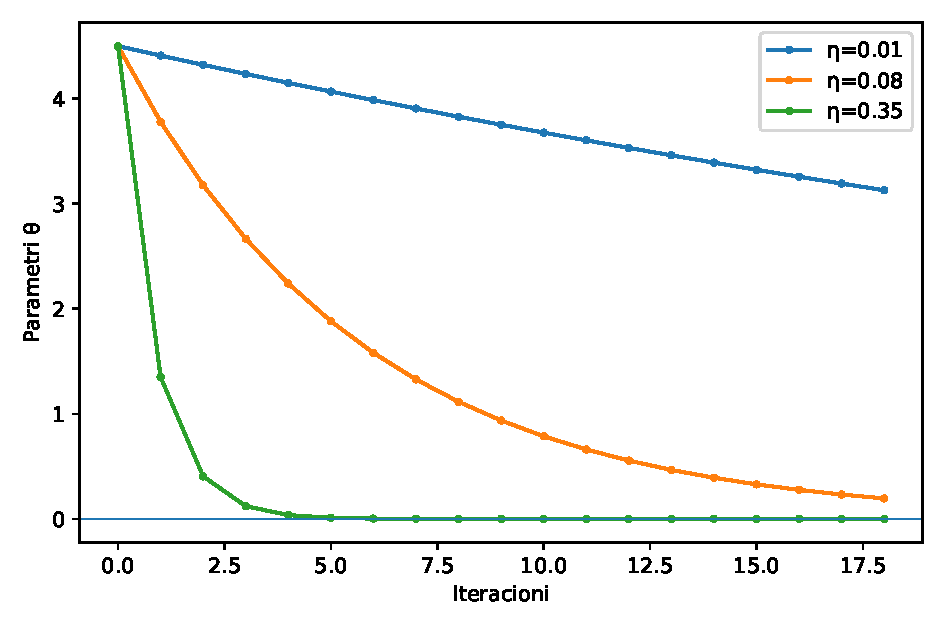
\includegraphics[width=.67\textwidth]{figures/fig_gradient_convergence.pdf}\caption{Konvergjenca e zbritjes së gradientit për disa shpejtësi të nxënit.}\label{fig:gd}\end{figure}

\section{Gradienti për regresionin linear dhe logjistik}

Për regresionin linear me MSE,
\[
\mathcal L(\boldsymbol\beta)=\frac1N\|X\boldsymbol\beta-\mathbf y\|^2,
\qquad
\nabla\mathcal L=\frac{2}{N}X^T(X\boldsymbol\beta-\mathbf y).
\]
Kjo na lejon të gjejmë numerikisht të njëjtën zgjidhje që më parë e morëm me ekuacionet normale. Ky krahasim është pedagogjikisht i fuqishëm: i njëjti problem ka zgjidhje analitike dhe iterative.

Për regresionin logjistik, gradienti i cross-entropy ka formën $X^T(\mathbf p-\mathbf y)/N$ (plus term regularizimi kur përdoret). Kështu gradient descent është urë midis regresionit klasik dhe klasifikimit probabilistik.

\section{Zbritja stokastike e gradientit}

Në \term{zbritjen stokastike të gradientit}{stochastic gradient descent, SGD}, gradienti vlerësohet nga një shembull ose minibashkësi e rastësishme. Kostoja për përditësim bie dhe zhurma e gradientit mund të ndihmojë lëvizjen në hapësirën e parametrave. Por trajektorja bëhet më e çrregullt dhe kërkon menaxhim të shpejtësisë së të nxënit.

Termi \emph{stokastik} këtu ka kuptim të saktë: përditësimi varet nga një mostër rastësore e të dhënave. Në praktikë përdoren minibatches që kombinojnë efikasitetin e operacioneve vektoriale me variabilitetin e SGD. Ky koncept përmendet këtu si metodë e përgjithshme optimizimi, jo si pronë ekskluzive e rrjetave nervore.

\section{Kondicionimi, shkallëzimi dhe diagnostika}

Nëse sipërfaqja e humbjes ka lakim shumë të ndryshëm në drejtime të ndryshme, gradient descent zigzagon dhe konvergon ngadalë. Standardizimi i veçorive e bën shpesh gjeometrinë më izotrope. Numri i kondicionimit i Hessianit në problem kuadratik është tregues i këtij vështirësimi.

Diagnoza praktike përfshin grafikun e humbjes ndaj iteracionit, normën e gradientit, ndryshimin e parametrave dhe performancën e validimit. Ndalimi nuk duhet bërë vetëm kur humbja e trajnimit vazhdon të ulet; për modele të fleksibël mund të monitorohet validimi.


\paragraph{Problem tipik në fizikë: përshtatja e një modeli jolinear.}
Nëse amplituda e një oscilatori të zbehur përshkruhet nga $A(t)=A_0e^{-\gamma t}$, parametrat $A_0$ dhe $\gamma$ mund të përcaktohen duke minimizuar shumën e katrorëve të rezidualeve. Kur modeli zgjerohet me parametra të tjerë ose kur zgjidhja analitike nuk është e leverdishme, zbritja e gradientit bëhet një mjet i drejtpërdrejtë për të lëvizur në hapësirën e parametrave.

\paragraph{Problem tipik jashtë fizikës: optimizimi i një modeli të kërkesës.}
Një model logjistik mund të parashikojë probabilitetin që një përdorues t'i përgjigjet një oferte. Koeficientët përcaktohen duke minimizuar entropinë e kryqëzuar. Nëse numri i të dhënave është shumë i madh, zbritja stokastike ose me minibashkësi shmang llogaritjen e gradientit mbi të gjithë bashkësinë në çdo hap. Kjo lidh drejtpërdrejt optimizimin numerik me shkallëzueshmërinë llogaritëse.

\begin{lstlisting}
theta = theta0.copy()
for step in range(n_steps):
    grad = gradient(theta, X, y)
    theta -= eta * grad
    if np.linalg.norm(grad) < tol:
        break
\end{lstlisting}
Ky kod është i thjeshtë, por diagnostika duhet të jetë më e pasur: duhet të ruhet humbja, norma e gradientit dhe, kur është e mundur, trajektorja e parametrave. Vetëm kështu mund të dallojmë konvergjencën nga stagnimi ose paqëndrueshmëria.

\section{Ushtrime}

\textbf{1.} Derivoni kushtin e konvergjencës për $\mathcal L=a\theta^2/2$. \textbf{2.} Implementoni gradient descent për regresion linear dhe krahasoni me OLS. \textbf{3.} Tregoni numerikisht efektin e standardizimit në numrin e iteracioneve. \textbf{4.} Implementoni SGD me batch=1 dhe minibatch=16. \textbf{5.} Shpjegoni pse një humbje që luhatet në SGD nuk nënkupton domosdoshmërisht dështim të optimizimit.


\paragraph{Gradienti dhe lakimi.}
Gradienti përmban vetëm informacion të rendit të parë. Në një funksion kuadratik $L=\tfrac12\theta^TH\theta$, drejtimet vetjake të Hessianit $H$ kanë lakime të ndryshme. Stabiliteti i gradient descent kërkon që learning rate të lidhet me vlerën vetjake më të madhe; shpejtësia e konvergjencës varet edhe nga raporti $\lambda_{\max}/\lambda_{\min}$, pra numri i kondicionimit. Kjo lidh optimizimin me algjebrën lineare të kapitujve të mëparshëm.

Standardizimi ndryshon gjeometrinë e problemit. Në regresion me një veçori në intervalin $10^{-3}$ dhe një tjetër në $10^4$, konturet e humbjes janë shumë të zgjatura. Një learning rate që është i sigurt në drejtimin e pjerrët është tepër i vogël në drejtimin e sheshtë. Pas standardizimit, konturet bëhen më afër rrethore dhe konvergjenca përshpejtohet.

\paragraph{Stopping criteria.}
Mund të ndalojmë kur ndryshimi relativ i humbjes është i vogël, kur norma e gradientit bie nën prag, ose pas një numri maksimal iteracionesh. Për modele ku overfitting është i mundur përdoret early stopping mbi validimin: ruhet modeli në iteracionin me performancën më të mirë të validimit. Në regresion linear konveks kjo nuk është zakonisht e nevojshme si regularizim, por ideja përgatit studentin për metoda më të avancuara.

\paragraph{SGD si vlerësues i gradientit.}
Në full-batch gradient përdorim të gjitha $N$ pikat, prandaj gradienti është i saktë për rrezikun empirik. Në SGD përdorim një pikë të rastësishme; pritja e gradientit stokastik është gradienti i plotë nëse mostrimi është uniform. Minibatch zvogëlon variancën e këtij vlerësuesi dhe shfrytëzon mirë llogaritjen vektoriale. Kështu batch size krijon kompromis midis zhurmës, kostos për hap dhe efikasitetit hardware.

\paragraph{Shembull i punuar: dy learning rates.}
Në funksionin $L(\theta)=5\theta^2/2$, update është $\theta_{n+1}=(1-5\eta)\theta_n$. Me $\eta=0.1$, faktori është 0.5 dhe konvergjenca është monotone. Me $\eta=0.3$, faktori është $-0.5$ dhe kemi oscilacion që zvogëlohet. Me $\eta=0.5$, faktori $-1.5$ jep divergjencë. Ky shembull bën të qartë pse ``learning rate më i madh'' nuk do të thotë ``më shpejt''.

\paragraph{Nga optimizimi te perceptroni dhe rrjetat.}
Perceptroni përdor update online vetëm për gabime dhe nuk minimizon cross-entropy. Regresioni logjistik minimizon një humbje të lëmuar me gradient. Rrjetat nervore të ardhshme do të përdorin të njëjtin koncept të optimizimit në një hapësirë parametrash shumë më të madhe. Kjo është arsyeja pse gradient descent vendoset para perceptronit në këtë kurs: ai është koncept i përgjithshëm numerik.

\paragraph{Diagnostika numerike.}
Një loss curve pa shkallë logaritmike mund të fshehë fazën e fundit të konvergjencës. Grafiku i normës së gradientit, learning rate dhe validation loss jep pamje më të plotë. Gjithashtu duhet kontrolluar që humbja nuk prodhon \texttt{nan} nga overflow ose logaritme të zeros. Stabiliteti numerik -- p.sh. clipping i logits ose përdorimi i funksioneve log-sum-exp -- është pjesë e implementimit profesional.

\chapter[Perceptroni]{Perceptroni dhe zhvillimet e mëtejshme}

Perceptroni është pika e fundit e trajtimit formal të këtij kursi dhe një urë natyrore drejt rrjetave nervore. Ai kombinon një shumë të ponderuar, një prag vendimi dhe një rregull të thjeshtë përditësimi. Kjo thjeshtësi e bën të mundur që të kuptojmë qartë çfarë mëson algoritmi, kur konvergon dhe pse dështon për probleme që nuk janë linearisht të ndashme.

Në një problem fizik dy klasa ngjarjesh mund të ndahen nga një kombinim linear i dy observablave. Në filtrimin e mesazheve, një model i ngjashëm mund të përdorë pesha të lidhura me praninë e fjalëve ose shenjave të caktuara. Për studentin, vlera kryesore e perceptronit është se hap rrugën për të kuptuar se rrjetat moderne nuk janë magji: ato ndërtojnë kompozime shumë më të pasura të të njëjtës ide bazë, me funksione aktivizimi të ndryshme dhe trajnim me gradient.
\section{Klasifikuesi linear si neuron artificial}

Perceptroni është pika e fundit e trajtimit formal të këtij kursi dhe një urë e natyrshme drejt rrjetave nervore. Ai llogarit një kombinim linear
\[
z=\mathbf w^T\mathbf x+b
\]

\paragraph{Interpretim.}
Shprehja është e njëjtë me pjesën lineare të regresionit logjistik dhe të SVM. Ajo përcakton një hiperplan $z=0$. Diferenca midis këtyre metodave nuk është te forma e hiperplanit, por te kriteri me të cilin ai gjendet: gjasa te regresioni logjistik, margjina te SVM dhe korrigjimi i gabimeve te perceptroni.
dhe merr vendim sipas shenjës së $z$. Në gjuhën e rrjetave, $\mathbf w$ quhen pesha, $b$ animi (bias) dhe funksioni i pragut është aktivizimi. Matematikisht, megjithatë, kemi ende një klasifikues linear.

Lidhja me regresionin logjistik është e drejtpërdrejtë: të dy përdorin të njëjtin $\mathbf w^T\mathbf x+b$, por regresioni logjistik e kalon në sigmoid dhe optimizon log-gjasën, ndërsa perceptroni përdor rregull përditësimi vetëm kur shembulli klasifikohet gabim.

\section{Rregulli i përditësimit}

Me etiketa $y_i\in\{-1,+1\}$, nëse $y_i(\mathbf w^T\mathbf x_i+b)\le0$, bëjmë
\[
\mathbf w\leftarrow\mathbf w+\eta y_i\mathbf x_i,
\qquad b\leftarrow b+\eta y_i.
\]
Ky rregull e shtyn hiperplanin në drejtim që favorizon klasifikimin e saktë të shembullit. Në variantin klasik $\eta$ mund të merret 1; shkalla ndikon në madhësinë e peshave por jo në ekzistencën e ndarjes kur të dhënat janë linearisht të ndashme.

Në notebook rregulli përkthehet pothuajse fjalë për fjalë në kod:
\begin{lstlisting}[caption={Përditësimi i perceptronit nga parimet e para.}]
for epoch in range(epochs):
    mistakes = 0
    for xi, yi in zip(X, y_signed):
        if yi * (w @ xi + b) <= 0:
            w += eta * yi * xi
            b += eta * yi
            mistakes += 1
    if mistakes == 0:
        break
\end{lstlisting}
Kjo transparencë është arsyeja pse perceptroni është një fund i mirë për kursin hyrës: studenti mund të lidhë gjeometrinë, algoritmin dhe kodin pa pasur ende nevojë për mekanizmin e prapapërhapjes.

Algoritmi është online: shembujt përpunohen një nga një dhe parametrat ndryshojnë menjëherë. Kjo e bën historikisht të rëndësishëm për sistemet e hershme të të nxënit dhe konceptualisht të dobishëm për të kuptuar algoritmet stokastike.

\section{Teorema e konvergjencës}

Supozoni se ekziston vektor njësi $\mathbf w^*$ që ndan shembujt me margjinë $\gamma>0$, pra $y_i\mathbf w^{*T}\mathbf x_i\ge\gamma$, dhe $\|\mathbf x_i\|\le R$. Teorema klasike e perceptronit tregon se numri i gabimeve është i kufizuar nga
\[
M\le\left(\frac{R}{\gamma}\right)^2.
\]
Ideja e provës ka dy hapa. Së pari, çdo përditësim rrit projeksionin $\mathbf w_t^T\mathbf w^*$ të paktën me $\gamma$, prandaj pas $M$ gabimeve ai është të paktën $M\gamma$. Së dyti, norma e $\mathbf w_t$ rritet jo më shpejt se $R\sqrt{M}$. Nga Cauchy--Schwarz, $M\gamma\le\|\mathbf w_M\|\le R\sqrt M$, prej nga del kufiri.

Teorema nuk thotë se perceptroni gjen kufirin me margjinën më të madhe, vetëm se do të gjejë një ndarje pas një numri të fundëm gabimesh kur ndarja ekziston. Kjo dallon qartë perceptronin nga SVM.

\section{Kufizimi themelor: XOR dhe jondashmëria lineare}

Perceptroni i vetëm nuk mund të përfaqësojë funksionin XOR. Pikat $(0,0)$ dhe $(1,1)$ i përkasin një klase, ndërsa $(0,1)$ dhe $(1,0)$ tjetrës; nuk ekziston vijë që i ndajë. Rritja e numrit të epokave nuk zgjidh një problem përfaqësimi.

Ky shembull është shumë i rëndësishëm pedagogjikisht: dështimi nuk vjen nga optimizimi, por nga klasa e hipotezave. Një transformim i veçorive mund ta bëjë problemin të ndashëm; për shembull, veçoria $x_1x_2$ shton jolinearitet. Rrjetat me shtresa të fshehta automatizojnë në njëfarë mase ndërtimin e përfaqësimeve jolineare, por ky zhvillim i takon kursit pasues.

\section{Nga perceptroni te rrjetat moderne: panoramë përshkruese}

Një \term{perceptron shumë-shtresor}{multilayer perceptron} kompozon transformime affine dhe funksione aktivizimi jolineare. Një shtresë mund të shkruhet
\[
\mathbf h=\phi(W\mathbf x+\mathbf b).
\]
Kompozimi i disa shtresave lejon kufij vendimi shumë më të pasur se një hiperplan. Parametrat përshtaten zakonisht me zbritje gradienti; \term{prapapërhapja}{backpropagation} është një mënyrë efikase për të zbatuar rregullin e zinxhirit dhe për të llogaritur gradientët. Në këtë kurs nuk e derivomë atë formalisht.

Rrjetat konvolucionale (CNN) shfrytëzojnë strukturën lokale dhe ndarjen e peshave në të dhëna hapësinore; rrjetat rekurrente modelojnë varësi sekuenciale; Transformer-at përdorin mekanizma attention dhe janë bërë arkitekturë qendrore për gjuhën dhe shumë probleme të tjera. Këto metoda nuk zëvendësojnë konceptet e këtij kursi. Përkundrazi, train/validation/test, regularizimi, optimizimi, rrjedhja e informacionit dhe interpretimi i metrikave bëhen edhe më të rëndësishme kur modelet rriten.


\paragraph{Problem tipik në fizikë: ndarja e dy familjeve të ngjarjeve.}
Marrim dy observabla, për shembull energjinë dhe një tregues të formës së impulsit. Nëse dy klasat ndahen nga një vijë, perceptroni mund të mësojë një kombinim linear të tyre. Kur një pikë klasifikohet gabim, pesha lëviz në drejtimin që e afron kufirin me një ndarje të saktë. Nëse klasat nuk janë linearisht të ndashme, rregulli vazhdon të përditësohet pa gjetur një zgjidhje perfekte; ky dështim është informacion mbi kapacitetin e modelit.

\paragraph{Problem tipik jashtë fizikës: filtrimi i mesazheve.}
Një paraqitje shumë e thjeshtë mund të përdorë veçori binare që tregojnë praninë e fjalëve ose strukturave të caktuara. Perceptroni ndërton një peshë për secilën veçori dhe merr vendim sipas shenjës së shumës së ponderuar. Ky shembull tregon se neuroni artificial është fillimisht një klasifikues linear; kompleksiteti i rrjetave të mëvonshme lind nga kombinimi i shumë njësive dhe jo nga ndryshimi i parimit bazë të peshimit.

\begin{figure}[H]\centering
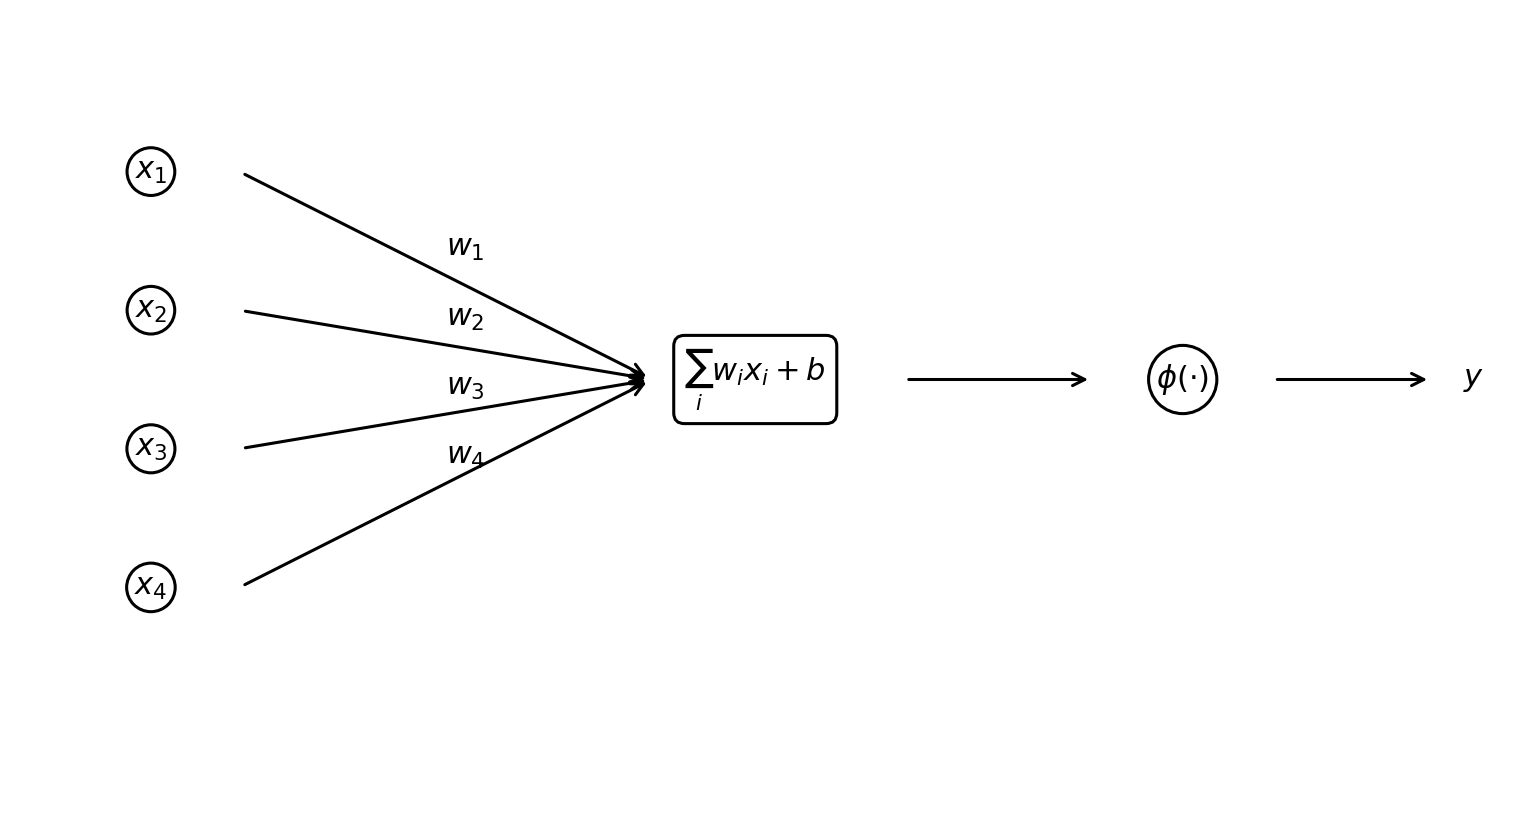
\includegraphics[width=.78\textwidth]{fig_perceptron_cc0_adapted.png}
\caption{Skema e një perceptroni me hyrje, pesha, shumën e ponderuar dhe funksionin e aktivizimit. Rivizatim i përshtatur nga figura e lirë \emph{Perceptron-unit.svg}, Wikimedia Commons, CC0. \url{https://commons.wikimedia.org/wiki/File:Perceptron-unit.svg}.}
\end{figure}

\begin{lstlisting}
for x_i, y_i in zip(X, y):
    pred = 1 if (x_i @ w + b) >= 0 else -1
    if pred != y_i:
        w += eta * y_i * x_i
        b += eta * y_i
\end{lstlisting}
Rregulli i përditësimit është i lexueshëm pikërisht sepse modeli është i thjeshtë. Kjo transparencë e bën perceptronin një fund të përshtatshëm për kursin Bachelor dhe një pikënisje të mirë për rrjetat nervore në ciklin Master.

\section{Shembull, krahasim dhe ushtrime përfundimtare}

Notebook-u për perceptronin do të përdorë fillimisht të dhëna fizikisht të interpretueshme dhe linearisht të ndashme. Algoritmi do të implementohet nga e para dhe do të regjistrohet numri i gabimeve në çdo epokë. Pastaj rezultati krahasohet me \texttt{sklearn.linear\_model.Perceptron} dhe me regresionin logjistik. Në fund përdoret XOR për të demonstruar kufirin e përfaqësimit.

\textbf{Ushtrime.} (i) Derivoni hapat kryesorë të teoremës së konvergjencës. (ii) Ndërtoni një bashkësi ku margjina zvogëlohet dhe vëzhgoni rritjen e numrit të gabimeve. (iii) Krahasoni kufirin e perceptronit me SVM në të njëjtat të dhëna. (iv) Shpjegoni pse sigmoid + cross-entropy jep interpretim probabilistik ndërsa perceptroni jo. (v) Shkruani me fjalë se çfarë problemi zgjidh një shtresë e fshehtë në rastin XOR, pa përdorur formalizmin e backpropagation.



\paragraph{Perceptroni si algoritëm online.}
Në secilin gabim, update varet vetëm nga shembulli aktual. Kjo e bën perceptronin të përshtatshëm për të dhëna që vijnë në rrjedhë dhe historikisht e lidh me idenë e të nxënit online. Rendi i shembujve mund të ndryshojë trajektoren dhe zgjidhjen përfundimtare, edhe pse teorema garanton konvergjencë kur ka ndashmëri lineare. Për këtë arsye në notebook përdoret shuffle me farë të kontrolluar dhe studiohet variabiliteti i numrit të gabimeve.

\paragraph{Teorema e konvergjencës në më shumë detaj.}
Pas $M$ gabimeve, projeksioni mbi ndarësin ideal rritet të paktën $M\gamma$. Nga ana tjetër, në një update të gabuar kemi $y_t w_t^Tx_t\le0$, prandaj
\[
\|w_{t+1}\|^2=\|w_t\|^2+2y_tw_t^Tx_t+\|x_t\|^2\le\|w_t\|^2+R^2.
\]
Pas $M$ gabimeve, $\|w_M\|\le R\sqrt M$. Me Cauchy--Schwarz,
$M\gamma\le w_M^Tw^*\le\|w_M\|$, dhe rezulton $M\le(R/\gamma)^2$. Ky argument është shembull i bukur i lidhjes midis gjeometrisë dhe garancisë algoritmike.

\paragraph{Çfarë nuk garanton teorema.}
Nëse të dhënat nuk janë të ndashme, perceptroni mund të vazhdojë pafund duke cikluar. Nëse ndarja ekziston por margjina është shumë e vogël, kufiri teorik i gabimeve mund të jetë i madh. Dhe edhe kur konvergon, zgjidhja nuk është domosdoshmërisht ajo me margjinë më të madhe. Kjo motivon SVM, e cila e formulon margjinën si objektiv explicit.

\paragraph{XOR dhe përfaqësimi.}
XOR tregon se problemi nuk është mungesa e kohës së trajnimit. Në hapësirën $(x_1,x_2)$ klasat janë të alternuara në cepat e katrorit dhe nuk ka hiperplan. Nëse shtojmë veçorinë $x_1x_2$, pikat vendosen në një hapësirë ku ndarja mund të bëhet lineare. Kjo ide -- transformimi i përfaqësimit -- është themelore në nxënien e thellë. Rrjetat shumë-shtresore mësojnë transformime të ndërmjetme në vend që t'i përcaktojë njeriu të gjitha veçoritë.

\paragraph{Panorama e rrjetave nervore pa hyrë në kursin pasues.}
Në MLP, çdo shtresë bën $h^{(l)}=\phi(W^{(l)}h^{(l-1)}+b^{(l)})$. Pa funksion jolinear, kompozimi i shtresave do të ishte përsëri transformim linear dhe nuk do të zgjidhte XOR në mënyrë më të fuqishme. Jolinearitetet si ReLU e ndryshojnë klasën e funksioneve. Backpropagation llogarit gradientët me rregullin e zinxhirit, por derivimi i plotë lihet për kursin Master. CNN shtojnë strukturë lokale dhe sharing të peshave; Transformer përdorin attention për ndërveprime midis elementeve të sekuencës. Këto janë zhvillime të së njëjtës filozofi: përfaqësim + funksion humbjeje + optimizim + validim.

\paragraph{Çfarë duhet të marrë studenti nga kursi.}
Qëllimi nuk është që studenti të dalë me listë algoritmesh. Ai duhet të jetë në gjendje të shohë një problem të ri fizik dhe të pyesë: çfarë është objektivi; cilat veçori janë legjitime; si ndahet dataset-i; cili baseline është i arsyeshëm; a kërkon problemi model linear, lokal, pemë, kernel, reduktim dimensional ose clustering; si do të matet pasiguria; dhe çfarë kufizimesh ka interpretimi. Perceptroni mbyll kursin sepse tregon se konceptet e mësuara -- lineariteti, humbja, margjina, optimizimi, ndashmëria dhe përfaqësimi -- janë pikërisht themeli mbi të cilin ndërtohen rrjetat nervore.

\appendix
\chapter[Algjebër lineare]{Përmbledhje e algjebrës lineare}
\section{Vektorë, norma dhe produkte skalare}
Për një vektor $\mathbf x\in\R^d$, norma Euklidiane është $\|\mathbf x\|_2=\sqrt{\mathbf x^T\mathbf x}$. Produkti skalar lidhet me këndin përmes $\mathbf x^T\mathbf z=\|\mathbf x\|\|\mathbf z\|\cos\theta$. Ortogonaliteti, projeksionet dhe bazat ortonormale janë qendrore për regresionin dhe PCA.
\section{Vlera vetjake dhe SVD}
Për matricë simetrike $C$, vlerat vetjake janë reale dhe ekziston bazë ortonormale vektorësh vetjakë. SVD shkruan $X=U\Sigma V^T$ dhe përdoret si mjet numerik stabil për katrorët më të vegjël dhe PCA.
\chapter[Probabilitet dhe statistikë]{Përmbledhje probabiliteti dhe statistike}
\section{Mesatarja, varianca dhe kovarianca}
$\E[X]$ përshkruan qendrën e shpërndarjes, $\Var(X)=\E[(X-\E X)^2]$ shpërndarjen, ndërsa kovarianca mat bashkë-variacionin linear. Korelacioni është kovariancë e normalizuar dhe nuk nënkupton kauzalitet.
\section{Gjasat dhe vlerësimi}
Maksimumi i gjasës zgjedh parametrat që e bëjnë kampionin e vëzhguar më të mundshëm nën model. Regresioni logjistik dhe shumë metoda klasifikimi mund të kuptohen nga ky këndvështrim.
\chapter[Riprodhueshmëria]{Eksperimente të riprodhueshme}
Ruani konfigurimin e mjedisit, versionet e bibliotekave, farat e rastësisë dhe kodin që gjeneron çdo figurë. Mos ruani vetëm një notebook të ekzekutuar: siguroni që ai të mund të ekzekutohet nga fillimi në fund në një mjedis të pastër. Për të dhënat e jashtme dokumentoni origjinën, licencën, njësitë dhe çdo filtrim.

\chapter[Studime të zgjeruara]{Studime të zgjeruara}
Ky shtojcë nuk shton tema të reja në program. Ajo rimerr dymbëdhjetë temat e kursit në formën e studimeve të zgjatura, me qëllim që studenti të shohë se si ndryshon mënyra e të menduarit kur një algoritëm vendoset brenda një problemi shkencor real. Çdo studim nis nga një pyetje fizike, përcakton të dhënat dhe kufizimet e matjes, formulon modelin, zgjedh procedurën e validimit dhe përfundon me një interpretim që dallon qartë atë që mbështetet nga të dhënat prej asaj që mbetet supozim.

\subsection*{Studim 1: nga pulsimi i detektorit te një problem i mirëformuluar i nxënies automatike}
Supozojmë se një detektor regjistron për çdo ngjarje një sinjal tensioni $V(t)$ në një dritare kohore të shkurtër. Qëllimi është të dallohen ngjarjet e interesit nga sfondi. Gabimi i parë që mund të bëhet është të hidhet i gjithë vektori i mostrave në një klasifikues pa u pyetur se çfarë përfaqësojnë fizikisht kolonat. Një mënyrë më e shëndoshë është të fillohet nga mekanizmi: amplituda maksimale lidhet me energjinë e depozituar, integrali i pulsit me ngarkesën totale, koha e ngritjes me dinamikën e formimit të sinjalit, ndërsa luhatja para pulsit jep një masë të zhurmës bazë. Kështu ndërtohet një tabelë me veçori që kanë njësi dhe kuptim.

Hapi i dytë është të përcaktohet njësia statistikore e pavarur. Nëse mijëra pulse vijnë nga i njëjti sesion eksperimental, ndarja e rastësishme e pulseve mund të bëjë që trajnimi dhe prova të përmbajnë të njëjtin drift instrumental. Performanca do të duket më e mirë se aftësia reale për të përgjithësuar në një sesion të ri. Prandaj, nëse identiteti i sesionit është i disponueshëm, ndarja duhet të bëhet sipas sesionit. Ky është një shembull tipik ku njohuria fizike përcakton skemën statistikore.

Përpunimi paraprak duhet të mësohet vetëm nga bashkësia e trajnimit. Nëse mesatarja dhe devijimi standard llogariten mbi të gjithë dataset-in para validimit të kryqëzuar, informacioni nga fold-et e validimit hyn në transformim. Edhe kur efekti numerik është i vogël, procedura është konceptualisht e gabuar. Për këtë arsye përdorim një \emph{pipeline}: standardizim dhe klasifikues trajnohen së bashku brenda çdo fold-i. Një eksperiment didaktik i dobishëm është të krijohet qëllimisht një veçori me shumë zhurmë, të zgjidhen veçoritë duke përdorur të gjithë dataset-in dhe të krahasohet rezultati me përzgjedhjen brenda pipeline-it; rritja artificiale e performancës e bën rrjedhjen e informacionit të dukshme.

Së fundi, metrika duhet të lidhet me qëllimin shkencor. Nëse sinjali është i rrallë, saktësia nuk është e mjaftueshme. Një analizë mund të ketë nevojë për recall të lartë për të mos humbur ngjarje, ose për precision të lartë për të shmangur një numër të madh kandidatësh të rremë. Pragu i klasifikimit nuk është ligj natyre; ai është pjesë e vendimit eksperimental. Ky studim përmbledh idenë kryesore të temës së parë: pyetja, struktura e të dhënave dhe protokolli i validimit duhet të përcaktohen para se të krahasohen algoritmet.

\subsection*{Studim 2: vlerësimi i konstantës së sustës me regresion linear}
Marrim një sustë që punon në regjimin elastik dhe matim zgjatjen $x$ për forca të ndryshme $F$. Modeli ideal është $F=kx$, por një eksperiment real mund të ketë edhe një offset të vogël nga zeroja e sensorit, prandaj modeli praktik shkruhet $F=\beta_0+\beta_1x+\epsilon$. Koeficienti $\beta_1$ vlerëson konstantën $k$ dhe intercepti $\beta_0$ shërben si kontroll diagnostik. Në formë matricore, me kolonë njësh dhe kolonën e zgjatjeve, vlerësimi i katrorëve më të vegjël është
\[
\hat\beta=(X^TX)^{-1}X^T y,
\]
kur matrica është e rangut të plotë. Në praktikë përdoret zgjidhje numerikisht më stabile me QR ose SVD, por formula mbetet thelbësore për interpretimin.

Një vlerë e vogël e MSE nuk provon ligjin e Hukut. Duhet të shihen mbetjet $r_i=F_i-\hat F_i$. Nëse mbetjet shfaqin lakim sistematik në zgjatje të mëdha, atëherë modeli linear po aplikohet jashtë regjimit elastik. Nëse dispersioni rritet me forcën, supozimi i variancës konstante mund të jetë i papërshtatshëm. Nëse matjet janë përsëritje të shpejta me të njëjtën pajisje, mbetjet mund të jenë të korreluara. Diagnostika e mbetjeve është pra pjesë e fizikës së problemit, jo vetëm kontroll statistik.

Pasiguria e koeficientëve mund të vlerësohet, nën supozimet klasike, nga
\[
\mathrm{Cov}(\hat\beta)=\hat\sigma^2(X^TX)^{-1}.
\]
Kjo formulë tregon drejtpërdrejt pse shpërndarja e pikave të $x$ ka rëndësi. Nëse të gjitha zgjatjet janë pothuajse të njëjta, elementi përkatës i $(X^TX)^{-1}$ rritet dhe vlerësimi i pjerrësisë bëhet i pasigurt. Kështu dizajni i eksperimentit dhe vlerësimi statistikor nuk janë dy faza të ndara: zgjedhja e pikave të matjes përcakton sa mirë mund të vlerësohet parametri fizik.

Një zgjerim i dobishëm është rasti kur pasiguria e forcës ndryshon nga një pikë në tjetrën. Atëherë katrorët e vegjël të ponderuar përdorin pesha $w_i\propto1/\sigma_i^2$. Nëse edhe $x$ ka pasiguri të konsiderueshme, regresioni standard nuk është më plotësisht i përshtatshëm dhe kërkohet model i gabimeve në të dy boshtet. Ky kufi metodologjik është i rëndësishëm për studentët e fizikës: nxënia automatike nuk i anulon parimet e metrologjisë.

\subsection*{Studim 3: kalibrimi jolinear, kompleksiteti dhe regularizimi}
Supozojmë një sensor temperature me përgjigje paksa jolineare. Të dhënat e kalibrimit janë çifte $(T_i,V_i)$ dhe synojmë të parashikojmë temperaturën nga tensioni. Një polinom me shkallë $p$ përfaqësohet si model linear në parametrat e tij, sepse matrica e dizajnit përmban kolonat $1,V,V^2,\ldots,V^p$. Kjo është një mundësi e mirë për të dalluar linearitetin në parametra nga lineariteti i formës së funksionit.

Kur $p$ rritet, gabimi i trajnimit zakonisht zvogëlohet. Megjithatë, kurba e validimit mund të ketë minimum dhe pastaj të rritet: modeli po përdor lirinë shtesë për të ndjekur zhurmën. Për një kalibrim fizik kjo mund të jetë veçanërisht e rrezikshme në skajet e intervalit, ku polinomi i shkallës së lartë mund të luhatet fort. Prandaj shkalla nuk zgjidhet duke parë vetëm përshtatjen vizuale në të dhënat e trajnimit; përdoret validim i kryqëzuar dhe kontroll i sjelljes jashtë pikave të dendura.

Regularizimi Ridge zgjidh
\[
\min_\beta \|y-X\beta\|_2^2+\lambda\|\beta\|_2^2,
\]
dhe zvogëlon koeficientët e drejtimeve të dobëta. Në bazën e vektorëve singularë, kjo mund të shihet si filtrim: komponentët që lidhen me vlera singulare të vogla shtypen më fort. Kjo është arsyeja pse Ridge përmirëson stabilitetin kur kolonat polinomiale janë fort të korreluara. Lasso përdor normën $L_1$ dhe mund të vendosë koeficientë ekzaktësisht në zero, por për veçori të korreluara përzgjedhja mund të jetë jo stabile.

Në laborator duhet të krahasohen jo vetëm gabimet, por edhe koeficientët si funksion i $\lambda$, kushtëzimi i matricës, dhe sjellja e modelit në një interval pak më të gjerë se kalibrimi. Një model me gabim validimi minimal por me divergjencë të fortë menjëherë jashtë intervalit mund të jetë zgjedhje e keqe për përdorim instrumental. Ky studim e lidh regularizimin me një ide fizike të njohur: një zgjidhje e qëndrueshme është shpesh më e vlefshme se një përshtatje tepër e ndjeshme ndaj zhurmës.

\subsection*{Studim 4: klasifikimi i pulseve dhe probabiliteti logjistik}
Konsiderojmë dy lloje pulses: sinjal dhe sfond. Për secilin puls përdorim amplitudën, integrimin dhe kohën e ngritjes. Regresioni logjistik modelon probabilitetin e klasës pozitive si
\[
p(y=1\mid x)=\sigma(w^Tx+b),\qquad \sigma(z)=\frac1{1+e^{-z}}.
\]
Ky interpretim probabilistik e dallon nga një rregull i thjeshtë me prag. Parametrat zgjidhen duke minimizuar entropinë e kryqëzuar, e cila del natyrshëm nga maksimumi i gjasës për variabla Bernoulli.

Në një eksperiment real, probabiliteti i parashikuar nuk përdoret domosdoshmërisht me pragun 0.5. Nëse kostoja e humbjes së një ngjarjeje është shumë e madhe, pragu mund të ulet për të rritur recall. Nëse verifikimi i çdo kandidati është i shtrenjtë, mund të kërkohet precision më i lartë. ROC tregon kompromisin midis true-positive rate dhe false-positive rate për pragje të ndryshme; precision-recall është shpesh më informuese kur klasa pozitive është e rrallë.

Kalibrimi është një dimension tjetër i cilësisë. Një model mund të rendisë saktë ngjarjet dhe të ketë AUC të lartë, por probabilitetet e tij të jenë tepër të sigurta. Nëse midis ngjarjeve me probabilitet të parashikuar 0.8 vetëm 60\% janë vërtet pozitive, modeli nuk është i kalibruar. Për përdorime ku probabiliteti futet më tej në një analizë fizike, kalibrimi ka rëndësi direkte.

Interpretimi i koeficientëve duhet të bëhet pas standardizimit me kujdes. Shenja e një koeficienti tregon drejtimin e efektit duke mbajtur veçoritë e tjera fikse, por ky kusht mund të mos jetë fizikisht i realizueshëm kur veçoritë janë të korreluara. Prandaj koeficientët janë dritare mbi modelin, jo prova kauzale. Në notebook duhet të krahasohet modeli manual me \texttt{LogisticRegression}, të kontrollohet konvergjenca, të ndryshohet pragu dhe të studiohet ndikimi i pabalancimit të klasave.

\subsection*{Studim 5: klasifikimi lokal i regjimeve dinamike me $k$-NN}
Marrim trajektore të një sistemi dinamik dhe prej secilës llogarisim energjinë mesatare, variancën, një frekuencë dominuese dhe një masë të korrelacionit. Synimi është të dallohen dy ose më shumë regjime. Metoda $k$-NN nuk mëson koeficientë globalë; ajo e përcakton klasën e pikës së re nga fqinjët më të afërt. Kështu nocioni i distancës bëhet vetë pjesë e modelit.

Nëse energjia matet në shkallë numerike shumë më të madhe se një koeficient i dimensionit pa njësi, distanca Euklidiane dominohet nga energjia. Standardizimi nuk është dekorim, por përcakton gjeometrinë. Në fizikë mund të kemi edhe njohuri që sugjeron një metrikë tjetër, por për nivelin hyrës është thelbësore të shihet qartë se ndryshimi i njësive mund të ndryshojë klasifikimin nëse veçoritë nuk shkallëzohen.

Vlera e $k$ kontrollon kompromisin bias-variancë. Me $k=1$ kufiri i vendimit mund të ndjekë çdo pikë të zhurmshme. Me $k$ shumë të madh, struktura lokale humbet. Vlera zgjidhet me validim të kryqëzuar vetëm në të dhënat e trajnimit. Një grafik i performancës kundrejt $k$ është shembull tipik i kurbës së validimit.

Mallkimi i dimensionalitetit shfaqet kur shtohen shumë veçori zhurme. Distancat midis pikave bëhen relativisht më të ngjashme dhe koncepti i fqinjit më të afërt humbet forcë. Në notebook mund të shtohen gradualisht kolona me zhurmë dhe të matet degradimi. Ky eksperiment jep një mësim më të gjerë: më shumë veçori nuk do të thotë automatikisht më shumë informacion të përdorshëm.

\subsection*{Studim 6: fazat e materialit, pemët dhe ansamblet}
Supozojmë se për mostra materiali maten dendësia, fortësia, përçueshmëria elektrike dhe një indikator strukturor, ndërsa etiketa tregon fazën. Një pemë vendimi ndan hapësirën me rregulla të tipit $x_j<c$. Çdo ndarje zgjidhet për të ulur papastërtinë e nyjeve, p.sh. papastërtinë Gini
\[
G=1-\sum_k p_k^2.
\]
Kjo e bën pemën të interpretueshme: një degë mund të lexojë afërsisht “përçueshmëri e lartë dhe fortësi mbi prag”.

Pema e thellë ka variancë të lartë. Ndryshimi i disa pikave mund të ndryshojë ndarjet e sipërme dhe kështu një pjesë të madhe të strukturës. Bagging e zvogëlon këtë variancë duke trajnuar shumë pemë mbi mostra bootstrap dhe duke mesatarizuar. Random Forest shton rastësi edhe në zgjedhjen e veçorive, duke ulur korrelacionin midis pemëve. Në shumë të dhëna tabelare kjo jep baseline shumë të fortë.

Megjithatë, interpretimi i rëndësisë së veçorive kërkon kujdes. Importanca e bazuar në uljen e impurity mund të favorizojë veçori me shumë pika prerjeje. Permutation importance mat rënien e performancës kur një kolonë përzihet, por edhe kjo ndikohet nga korrelacioni midis veçorive. Dy matje që përmbajnë të njëjtin informacion fizik mund ta “ndajnë” rëndësinë.

Boosting ka filozofi tjetër: modelet ndërtohen në seri dhe çdo hap përqendrohet te gabimet e ansamblit aktual. Në kurs mjafton të kuptohet kjo ide dhe të shihet praktikisht një algoritëm i gatshëm; derivimi i plotë i gradient boosting nuk është i domosdoshëm. Për studentin është më e rëndësishme të kuptojë pse ansambli mund të ulë gabimin dhe çfarë humbet në interpretueshmëri e kosto.

\subsection*{Studim 7: SVM dhe ndarja e regjimeve në hapësirën e fazës}
Në një sistem dinamik mund të nxjerrim dy veçori nga trajektorja dhe të kërkojmë ndarjen e dy regjimeve. Nëse klasat janë linearisht të ndashme, SVM zgjedh hiperplanin me margjinë maksimale. Pikat që prekin ose përcaktojnë margjinën janë vektorët mbështetës; pjesa tjetër e të dhënave ndikon vetëm indirekt. Kjo varësi e rrallë nga pikat kritike jep interpretim gjeometrik të fortë.

Për të dhëna me mbivendosje përdoret margjina e butë. Parametri $C$ kontrollon sa kushton shkelja e margjinës. $C$ shumë i madh mund të përpiqet të klasifikojë edhe outlier-at, duke prodhuar kufi kompleks; $C$ i vogël toleron më shumë shkelje dhe regularizon. Në notebook duhet të vizatohen kufijtë për disa vlera të $C$, jo vetëm të raportohet saktësia.

Kerneli RBF zëvendëson produktin skalar me masë ngjashmërie jolineare. Parametri $\gamma$ përcakton shkallën hapësinore: $\gamma$ i madh krijon ndikim shumë lokal dhe mund të japë kufi të dredhur; $\gamma$ i vogël jep kufi më të butë. $C$ dhe $\gamma$ duhen zgjedhur së bashku me validim të kryqëzuar. Kjo është një mundësi e mirë për të demonstruar një hartë dy-dimensionale të rezultatit të validimit.

Standardizimi është i domosdoshëm sepse margjina dhe RBF varen nga distancat. Për një student fizike është e dobishme të interpretojë vektorët mbështetës si raste eksperimentale “në kufi” midis regjimeve. Inspektimi i tyre mund të zbulojë nëse paqartësia është vërtet fizike apo vjen nga etiketime të dobëta.

\subsection*{Studim 8: PCA e spektrave dhe kuptimi i komponentëve}
Konsiderojmë $N$ spektre të matur në $d$ gjatësi vale. Çdo spektër është pikë në $\mathbb R^d$, por shumë dimensione janë fort të korreluara sepse ndryshimet fizike janë të kontrolluara nga pak parametra, si temperatura, amplituda ose përbërja. Pas qendërzimit, PCA diagonalizon matricën e kovariancës
\[
C=\frac1{N-1}X^TX,
\qquad Cv_i=\lambda_i v_i.
\]
Vektorët $v_i$ janë drejtime ortogonale me varianca të renditura nga $\lambda_i$.

Për spektre, loading-et e komponentit të parë mund të duken si ndryshim i amplitudës së përgjithshme; i dyti mund të theksojë zhvendosjen e një vije ose ndryshim të pjerrësisë. Kjo nuk duhet interpretuar automatikisht si “komponenti 1 është temperatura”. PCA optimizon variancën, jo domethënien fizike. Për të bërë lidhjen me një parametër duhet korelacion i jashtëm ose model fizik.

Numri i komponentëve mund të zgjidhet nga varianca e shpjeguar ose nga gabimi i rindërtimit. Megjithatë, 95\% variancë nuk është rregull universal. Një sinjal i rrallë fizik mund të ketë variancë të vogël dhe të bjerë në komponentët e vonshëm. Prandaj qëllimi i analizës duhet të përcaktojë kriterin.

Implementimi manual kalon nga qendërzimi te kovarianca, diagonalizimi, renditja e vlerave vetjake dhe projekcioni. Krahasimi me \texttt{sklearn.decomposition.PCA} dhe me SVD tregon se rezultatet mund të ndryshojnë në shenjën e vektorëve pa ndryshuar nënhapësirën. Kjo është një pikë numerike që duhet shpjeguar, që studentët të mos e konsiderojnë ndryshimin e shenjës si mospërputhje algoritmike.

\subsection*{Studim 9: zbulimi i regjimeve atmosferike me grupim}
Supozojmë matje ditore të temperaturës, presionit, lagështisë dhe erës. Nuk kemi etiketa “regjim 1/2/3”; kërkojmë nëse ekziston strukturë e përsëritur. $k$-means minimizon shumën e distancave katrore ndaj centroidëve. Hapi i caktimit dhe hapi i përditësimit ulin objektivin në mënyrë monotone, por zgjidhja mund të varet nga inicializimi.

Standardizimi është kritik sepse temperatura në gradë, presioni në hPa dhe era në m/s kanë shkallë të ndryshme. Pas shkallëzimit, një ndarje mund të interpretohet duke kthyer centroidët në njësitë origjinale. Për shembull, një grup mund të karakterizohet nga presion i lartë dhe erë e dobët. Kjo është shumë më e dobishme se të shihen vetëm etiketat numerike 0, 1, 2.

Metoda e bërrylit dhe silhouette ndihmojnë në zgjedhjen e $k$, por nuk japin “numrin e vërtetë” të regjimeve. Grupimi hierarkik mund të tregojë se struktura është shumëshkallëshe: dy makro-regjime që ndahen secili në nënregjime. Dendrograma është kështu mjet eksplorimi, jo thjesht grafik dekorativ.

Një kontroll i rëndësishëm është stabiliteti. Nëse ndryshimi i farës ose heqja e 5\% të pikave ndryshon rrënjësisht grupet, interpretimi fizik duhet të jetë i rezervuar. Po ashtu, $k$-means preferon grupe afërsisht sferike; për forma hënore ose dendësi shumë të ndryshme dështimi është i pritshëm. Në notebook duhet të përfshihet qëllimisht një rast ku algoritmi dështon, sepse të kuptuarit e kufirit të metodës është po aq i rëndësishëm sa aplikimi i suksesshëm.

\subsection*{Studim 10: krahasimi i modeleve si eksperiment shkencor}
Marrim një dataset të vetëm të pulsimit të detektorit dhe krahasojmë regresionin logjistik, $k$-NN, pemën, Random Forest dhe SVM. Të gjitha modelet duhet të marrin të njëjtat ndarje dhe të vlerësohen me të njëjtat fold-e; ndryshe ndryshimi i performancës përzihet me ndryshimin e mostrës. Për modelet që kërkojnë shkallëzim, transformimi vendoset në pipeline. Hiperparametrat zgjidhen vetëm brenda të dhënave të trajnimit.

Rezultati nuk duhet reduktuar në një tabelë me një kolonë accuracy. Për secilin model raportohen mesatarja dhe dispersioni i validimit, AUC ose metrika tjetër e përshtatshme, koha e trajnimit, ndjeshmëria ndaj zhurmës dhe interpretueshmëria. Një model pak më i dobët por shumë më stabil dhe transparent mund të jetë zgjedhja më e mirë për një analizë shkencore.

Bootstrap mbi bashkësinë e provës jep një ide të pasigurisë së metrikës. Për çdo rimarrje llogaritet AUC dhe nga shpërndarja ndërtohet interval. Ky interval nuk është pasiguri e plotë e të gjithë procesit, por i kujton studentit se “AUC=0.913” nuk është konstante fizike pa pasiguri.

Robustësia testohet duke shtuar zhurmë të kontrolluar, duke zhvendosur mesataret e veçorive brenda kufijve instrumentalë ose duke hequr një veçori. Nëse një model shembet nga perturbim shumë i vogël, kjo ka rëndësi praktike. Interpretimi plotësohet me koeficientë, strukturë peme, permutation importance ose vektorë mbështetës. Përfundimi duhet të argumentojë zgjedhjen në funksion të qëllimit, jo të shpallë një fitues absolut.

\subsection*{Studim 11: zbritja e gradientit, shkallëzimi dhe stabiliteti}
Marrim regresion linear me MSE. Gradienti ndaj parametrave është
\[
\nabla_\beta L=\frac{2}{N}X^T(X\beta-y),
\]
dhe përditësimi është $\beta_{t+1}=\beta_t-\eta\nabla L$. Në një problem ku një veçori është e rendit $10^{-3}$ dhe një tjetër $10^4$, niveli i funksionit të humbjes është shumë i zgjatur. Gradient descent zigzagon dhe kërkon learning rate të vogël. Standardizimi e bën gjeometrinë më izotrope dhe përshpejton konvergjencën.

Për funksion kuadratik, spektri i Hessian-it kontrollon shpejtësinë. Raporti $\lambda_{\max}/\lambda_{\min}$ është numri i kushtëzimit. Sa më i madh, aq më të ndryshme janë shkallët e lakimit. Kjo lidh drejtpërdrejt optimizimin me algjebrën lineare të mësuar në regresion dhe PCA.

Zbritja stokastike e gradientit përdor një shembull ose mini-batch për të vlerësuar gradientin. Vlerësimi është i zhurmshëm por më i lirë; zhurma mund të ndihmojë eksplorimin ndërsa learning rate zvogëlohet me kohën. Për kursin hyrës mjafton të krahasohen trajektoret batch, stochastic dhe mini-batch në të njëjtin problem dhe të diskutohet kompromisi midis kostos së një hapi dhe variancës së drejtimit.

Diagnostika përfshin loss curve, normën e gradientit, madhësinë e hapit dhe validimin. Divergjenca, oscilacionet ose plateau nuk duhen “rregulluar” duke provuar numra verbërisht; studentët duhet t'i lidhin me gjeometrinë e problemit. Kjo temë përgatit perceptronin dhe kursin e mëvonshëm të rrjetave nervore pa e kthyer optimizimin në një teknikë ekskluzive të Deep Learning.

\subsection*{Studim 12: perceptroni, margjina dhe kufiri i përfaqësimit}
Për një klasifikim binar me etiketa $y_i\in\{-1,+1\}$, perceptroni përdor shenjën e $w^Tx+b$. Kur një shembull klasifikohet gabim, parametrat përditësohen në drejtimin $y_ix_i$. Nëse të dhënat janë linearisht të ndashme me margjinë pozitive, algoritmi konvergon pas numri të fundëm gabimesh. Kufiri klasik
\[
M\le (R/\gamma)^2
\]
lidh numrin e gabimeve me normën maksimale të shembujve $R$ dhe margjinën $\gamma$.

Ky rezultat është i rëndësishëm jo sepse perceptroni është klasifikuesi më i mirë modern, por sepse tregon se mund të provohet marrëdhënia midis gjeometrisë së të dhënave dhe sjelljes së algoritmit. SVM e çon idenë më tej duke optimizuar margjinën; regresioni logjistik jep probabilitet; perceptroni mbetet një rregull i thjeshtë me përditësime online.

XOR demonstron kufirin e një klasifikuesi linear. Nuk ka numër epokash që ta zgjidhë pa ndryshuar përfaqësimin. Shtimi i veçorisë $x_1x_2$ ose përdorimi i një shtrese të fshehtë krijon një hapësirë ku ndarja mund të bëhet lineare. Kjo është ura konceptuale drejt rrjetave nervore: jo thjesht “më shumë parametra”, por mësim i përfaqësimeve jolineare.

Në përfundim përmenden perceptroni shumë-shtresor, prapapërhapja, CNN, rrjetat sekuenciale dhe Transformer-at pa derivime. Studenti duhet të largohet me idenë se konceptet e këtij kursi nuk hidhen poshtë nga Deep Learning: ndarja train/validation/test, regularizimi, optimizimi, rrjedhja e informacionit, metrikat dhe pasiguria bëhen edhe më kritike. Kjo është arsyeja pse perceptroni është pikë e mirë ndalimi për Bachelor-in dhe hyrje e mirë për trajtimin e ardhshëm në Master.

\chapter[Probleme të zgjidhura]{Probleme të zgjidhura dhe vetëstudim}
Problemet e mëposhtme janë menduar si material referimi. Zgjidhjet nuk zëvendësojnë punën e studentit; ato tregojnë se si argumentohet një zgjidhje e plotë, duke përfshirë jo vetëm llogaritjen por edhe kontrollin e supozimeve dhe interpretimin fizik.

\section{Probleme 1--2: validimi dhe regresioni}
\textbf{Problem 1.} Një laborator ka 6000 pulse të regjistruara në gjashtë ditë, 1000 pulse në ditë. Drift-i i bazës ndryshon nga dita në ditë. Propozoni një skemë validimi për një klasifikues sinjal/sfond.\\
\textbf{Zgjidhje.} Ndarja e rastësishme në nivel pulsi do të vendoste pulse të së njëjtës ditë në trajnim dhe validim; modeli mund të shfrytëzojë drift-in specifik të ditës. Njësia natyrore e grupimit është dita. Përdoret GroupKFold ose skemë leave-one-day-out; standardizimi dhe çdo përzgjedhje veçorish vendosen brenda pipeline-it. Një ditë mund të mbahet krejtësisht jashtë si provë përfundimtare. Ky protokoll mat aftësinë për të kaluar në një sesion të ri, që është pyetja reale.

\textbf{Problem 2.} Për matjet $(x,F)=(1,2.1),(2,4.0),(3,6.2),(4,7.9)$, përshtatni $F=\beta_0+\beta_1x$ dhe interpretoni $\beta_1$.\\
\textbf{Zgjidhje.} Pjerrësia mund të llogaritet nga $\hat\beta_1=\sum(x_i-\bar x)(F_i-\bar F)/\sum(x_i-\bar x)^2$. Kemi $\bar x=2.5$ dhe $\bar F=5.05$; numëruesi është afërsisht 9.75 dhe emëruesi 5, prandaj $\hat\beta_1\approx1.95$ në njësitë $F/x$. Intercepti është $\bar F-\hat\beta_1\bar x\approx0.175$. Nëse $F$ është N dhe $x$ është m, pjerrësia vlerëson $k\approx1.95\,\mathrm{N/m}$. Intercepti jo zero sugjeron offset ose zhurmë; duhet kontrolluar nëse është statistikisht dhe fizikisht domethënës.

\section{Probleme 3--4: regularizimi dhe klasifikimi probabilistik}
\textbf{Problem 3.} Shpjegoni pse Ridge ndihmon kur dy kolona të matricës së dizajnit janë pothuajse linearisht të varura.\\
\textbf{Zgjidhje.} Në OLS, drejtimet që korrespondojnë me vlera singulare shumë të vogla amplifikohen nga inversi. Koeficientët mund të marrin vlera të mëdha me shenja të kundërta, ndërsa parashikimi ndryshon shumë nga perturbime të vogla. Ridge zëvendëson faktorët $1/s_j$ me forma të shtypura, në mënyrë efektive duke mos lejuar amplifikim të pakufizuar të drejtimeve të dobëta. Çmimi është bias i vogël; fitimi është ulje e variancës dhe stabilitet më i madh.

\textbf{Problem 4.} Një klasifikues jep probability 0.3 për një ngjarje. A duhet ta quajmë sfond?\\
\textbf{Zgjidhje.} Jo pa specifikuar pragun dhe koston e gabimeve. Nëse pragu është 0.5, klasifikimi standard do të ishte sfond, por në një kërkim ku humbja e sinjalit është shumë e kushtueshme mund të përdoret 0.2. Probabiliteti dhe vendimi janë dy objekte të ndryshme. Për më tepër duhet verifikuar kalibrimi: 0.3 duhet të ketë kuptim empirik si frekuencë afërsisht 30\% për raste të ngjashme, nëse duam interpretim probabilistik të drejtpërdrejtë.

\section{Probleme 5--6: fqinjët dhe pemët}
\textbf{Problem 5.} Dy veçori kanë devijime standarde 0.02 dhe 50. Çfarë ndodh me $k$-NN pa standardizim?\\
\textbf{Zgjidhje.} Në distancën Euklidiane, ndryshimi tipik i veçorisë së dytë jep kontribut rreth $50^2$, ndërsa i pari rreth $0.02^2$. Praktikisht veçoria e parë injorohet, pavarësisht sa informative është fizikisht. Standardizimi i sjell të dyja në shkallë të krahasueshme. Nëse njësitë kanë kuptim të veçantë, mund të argumentohet metrikë e peshuar, por ajo duhet të justifikohet dhe validohet.

\textbf{Problem 6.} Pse një Random Forest zakonisht ka variancë më të vogël se një pemë e vetme?\\
\textbf{Zgjidhje.} Pemët e thella janë estimatorë me variancë të lartë. Mesatarizimi i shumë estimatorëve zvogëlon variancën; nëse varianca e secilës pemë është $\sigma^2$ dhe korrelacioni mes tyre $\rho$, varianca e mesatares për shumë pemë afrohet me $\rho\sigma^2$. Random Forest ul $\rho$ duke kufizuar rastësisht veçoritë e disponueshme në çdo ndarje, ndërsa bootstrap-i ndryshon mostrën. Prandaj ansambli stabilizohet pa rritur shumë bias-in.

\section{Probleme 7--8: SVM dhe PCA}
\textbf{Problem 7.} Çfarë prisni kur $C$ rritet shumë në soft-margin SVM?\\
\textbf{Zgjidhje.} Shkeljet e margjinës penalizohen fort. Modeli përpiqet të klasifikojë saktë sa më shumë pika trajnimi dhe mund të përdorë margjinë më të ngushtë. Në prani të outlier-ave kjo rrit ndjeshmërinë dhe rrezikun e mbipërshtatjes. $C$ i vogël lejon shkelje, jep margjinë më të gjerë dhe regularizim më të fortë. Vlera zgjidhet me validim, jo me parim absolut.

\textbf{Problem 8.} Pse PCA kërkon qendërzim?\\
\textbf{Zgjidhje.} PCA kërkon drejtime të variacionit rreth mesatares. Pa qendërzim, matrica $X^TX$ përmban edhe efektin e zhvendosjes së qendrës nga origjina; komponenti i parë mund të drejtohet kryesisht nga vektori i mesatares, jo nga kovarianca e luhatjeve. Qendërzimi e bën $X^TX/(N-1)$ matricë kovariance. Standardizimi, në dallim, nuk është gjithmonë i detyrueshëm dhe varet nga njësitë e kuptimi fizik.

\section{Probleme 9--10: grupimi dhe krahasimi i modeleve}
\textbf{Problem 9.} $k$-means jep silhouette të mirë për tre grupe. A kemi provuar se sistemi ka tri faza?\\
\textbf{Zgjidhje.} Jo. Silhouette mat kohezion dhe ndarje gjeometrike sipas metrikës së zgjedhur. Faza fizike kërkon evidencë të jashtme: sjellje të ndryshme të observablave, varësi sistematike nga parametrat e kontrollit, riprodhueshmëri dhe përputhje me teori. Grupimi është gjenerator hipotezash, jo provë e drejtpërdrejtë e ontologjisë fizike.

\textbf{Problem 10.} Dy modele kanë AUC $0.914\pm0.010$ dhe $0.919\pm0.012$. A është modeli i dytë domosdoshmërisht më i mirë?\\
\textbf{Zgjidhje.} Jo. Intervalet janë të mbivendosura dhe diferenca 0.005 mund të jetë brenda variabilitetit të mostrës. Duhet përdorur krahasim i çiftuar në të njëjtat fold-e ose bootstrap i diferencës së metrikës. Edhe nëse diferenca është e qëndrueshme, vendimi mund të varet nga kalibrimi, interpretueshmëria, kostoja dhe robustësia. Performanca numerike është vetëm një kriter.

\section{Probleme 11--12: optimizimi dhe perceptroni}
\textbf{Problem 11.} Për $L(\theta)=\tfrac12a\theta^2$, gjeni kushtin e konvergjencës së gradient descent me learning rate konstant.\\
\textbf{Zgjidhje.} Gradienti është $a\theta$, prandaj $\theta_{n+1}=(1-a\eta)\theta_n$. Konvergjenca kërkon $|1-a\eta|<1$, pra $0<\eta<2/a$. Për $0<\eta<1/a$ konvergjenca është monotone; për $1/a<\eta<2/a$ shfaqen oscilacione me amplitudë në zvogëlim. Ky rast një-dimensional shpjegon rolin e vlerave vetjake të Hessian-it në dimensione më të larta.

\textbf{Problem 12.} Pse perceptroni nuk zgjidh XOR dhe çfarë mësimi metodologjik jep kjo?\\
\textbf{Zgjidhje.} Perceptroni realizon vetëm kufi linear $w^Tx+b=0$. Katër pikat e XOR janë të alternuara dhe asnjë vijë nuk i ndan klasat. Dështimi vazhdon edhe me learning rate tjetër ose më shumë epoka; problemi është klasa e hipotezës, jo optimizimi. Shtimi i një veçorie jolineare ose i një shtrese të fshehtë ndryshon përfaqësimin. Mësimi është se para se të “tuning”-ojmë një algoritëm, duhet të pyesim nëse modeli ka kapacitetin strukturor për fenomenin.

\chapter[Diagnostika laboratorike]{Diagnostika e laboratorëve}
\section{Grafikët që duhet të lexohen, jo vetëm të prodhohen}
Një grafik regresioni duhet të shoqërohet me mbetjet; një confusion matrix duhet të lidhet me numrin real të ngjarjeve dhe jo vetëm me përqindje; ROC duhet të interpretohet në lidhje me prevalencën dhe koston e pragut; kurba e validimit duhet të tregojë se ku fillon mbipërshtatja. Në PCA, grafiku i variancës së shpjeguar pa loading-et jep vetëm gjysmën e historisë; në clustering, scatter plot i dy komponentëve të parë mund të fshehë strukturë që ekziston në dimensione të tjera. Qëllimi i laboratorëve është që studenti të mësojë të bëjë pyetje mbi figurën: çfarë sasie është në bosht, cilat njësi ka, çfarë do të ndryshonte nën një transformim të të dhënave dhe cilat përfundime nuk lejohen nga grafiku.

\section{Kontrolle negative dhe modele bazë}
Çdo pipeline duhet të ketë një baseline. Për regresion mund të jetë parashikimi me mesataren; për klasifikim klasa më e shpeshtë ose një rregull fizik i thjeshtë. Një model kompleks që nuk e kalon baseline-in nuk ka fituar asgjë. Kontrolli negativ shkon më tej: përziejmë etiketat dhe presim që performanca të bjerë në nivelin e rastësisë. Nëse mbetet e lartë, ka pothuajse me siguri rrjedhje informacioni ose gabim në pipeline. Kjo teknikë e thjeshtë është jashtëzakonisht e vlefshme në projekte studentore.

\section{Përsëritshmëria numerike}
Fara e rastësisë duhet të kontrollohet për ndarjet, inicializimet dhe bootstrap-in, por rezultati nuk duhet të varet nga një farë e vetme. Praktika e mirë është të raportohet variabiliteti në disa fara ose fold-e. Versionet e bibliotekave dokumentohen; notebook-u duhet të ekzekutohet nga fillimi në fund në kernel të pastër; qelizat nuk duhet të varen nga gjendje e fshehur e krijuar nga ekzekutim jashtë rendit. Nëse një rezultat ndryshon ndjeshëm me ndryshimin e vogël të farës, kjo është informacion mbi stabilitetin, jo bezdi që duhet fshehur.

\section{Si të shkruhet interpretimi shkencor}
Një interpretim i mirë dallon tri nivele: çfarë është vëzhguar, çfarë sugjeron modeli, dhe çfarë mekanizmi fizik mund ta shpjegojë. Për shembull: “Random Forest jep AUC më të lartë” është vëzhgim numerik; “marrëdhënia duket jolineare dhe me ndërveprime” është interpretim modelor; “ndërveprimi mund të lidhet me procesin X” është hipotezë fizike. Këto nuk duhet të bashkohen në një fjali kauzale pa evidencë shtesë. Ky disiplinim i gjuhës është pjesë e metodologjisë shkencore.

\section{Kur duhet të ndalojmë së rrituri kompleksitetin}
Kompleksiteti shtesë justifikohet kur adreson një mangësi të diagnostikuar dhe përmirëson performancën jashtë mostrës në mënyrë të qëndrueshme. Nëse SVM me RBF fiton shumë pak ndaj regresionit logjistik dhe kërkon tuning më delikat, mund të mos ketë arsye praktike për ta preferuar. Nëse PCA ul dimensionin pa humbur informacion relevant dhe përmirëson stabilitetin, është hap i arsyeshëm. Parimi është ekonomik: përdor modelin më të thjeshtë që i përgjigjet pyetjes me saktësi dhe robustësi të mjaftueshme.

\section{Lista e kontrollit para dorëzimit të një notebook-u}
Para dorëzimit duhet të kontrollohen: ndarja e të dhënave dhe mungesa e leakage; pipeline-i i transformimeve; baseline-i; metrika dhe arsyetimi i saj; variabiliteti i validimit; hiperparametrat dhe mënyra e zgjedhjes; figura me etiketa e njësi; kontrolli i rasteve të dështimit; interpretimi fizik; farat dhe versionet; ekzekutimi nga kernel i pastër. Nëse njëri prej këtyre elementeve mungon, analiza mund të jetë teknikisht e ekzekutueshme por shkencërisht e paplotë.

\chapter[Leksion--notebook]{Ura leksion--notebook}
Ky shtojcë përshkruan se si secila temë teorike shndërrohet në eksperiment numerik. Nuk është një manual i komandave Python; është një udhëzues për pyetjet që duhet të drejtojnë laboratorin.
\subsection*{Kapitulli 1: nga tabela e papërpunuar te eksperimenti i validueshëm}
Në laborator, tema e parë duhet të bëjë të dukshme se përpunimi i të dhënave është pjesë e modelit. Filloni me dataset-in e pulseve dhe ndani fillimisht një bashkësi prove që nuk preket më. Në pjesën e mbetur ndërtoni një pipeline me imputim, standardizim dhe një klasifikues të thjeshtë. Pastaj krijoni qëllimisht një version të gabuar ku standardizimi ose përzgjedhja e veçorive bëhet mbi të gjithë dataset-in. Krahasimi i rezultateve duhet të shoqërohet me shpjegimin se pse varianti i gabuar ka parë informacion nga validimi. Studentët duhet të identifikojnë jo vetëm rreshtin problematik të kodit, por edhe supozimin shkencor që shkelet.

Një detyrë e dytë është të ndryshohet njësia e grupimit. Krahasohet një ndarje e rastësishme e pulseve me një ndarje sipas sesionit. Nëse ka drift midis sesioneve, diferenca në performancë bëhet ilustrim i domain shift. Kjo e përgatit studentin për një parim që do të rikthehet vazhdimisht: mënyra e ndarjes duhet të imitojë mënyrën se si modeli do të ndeshë të dhëna të reja. Në fund të notebook-ut, studenti duhet të shkruajë me fjalë protokollin e validimit, jo vetëm të ekzekutojë funksione.

\subsection*{Kapitulli 2: regjimi linear si problem vlerësimi dhe diagnostike}
Notebook-u i regresionit linear duhet të ketë dy shtresa. Në të parën, zgjidhja ndërtohet nga algjebra lineare: matrica e dizajnit, ekuacionet normale, projeksioni dhe mbetjet. Në të dytën, i njëjti problem trajtohet si eksperiment fizik. Për të dhënat e ligjit të Hukut, studenti vlerëson konstantën e sustës, pasigurinë e saj dhe interceptin. Pastaj hiqen pikat e zgjatjes së vogël ose të madhe dhe kontrollohet stabiliteti. Nëse vlerësimi ndryshon dukshëm, kjo sinjalizon se rezultati varet nga diapazoni ose nga jolineariteti.

Një shembull i dytë me rënie të lirë përdor kolonat $1,t,t^2$. Ai tregon pse termi “regresion linear” do të thotë linear në parametra. Studentët duhet të provojnë model të gabuar vetëm me $t^2$, pastaj modelin fizikisht të plotë dhe të krahasojnë mbetjet. Kështu, notebook-u nuk demonstron vetëm formulën OLS; ai tregon se një algoritëm numerik nuk korrigjon një model fizik të keq. Në fund krahasohen zgjidhja manuale, \texttt{lstsq} dhe \texttt{LinearRegression}, me toleranca numerike të arsyetuara.

\subsection*{Kapitulli 3: kompleksiteti, regularizimi dhe ekstrapolimi}
Për kalibrimin e sensorit, notebook-u duhet të ndërtojë manualisht matricën polinomiale dhe të vizatojë njëkohësisht gabimin e trajnimit dhe të validimit kundrejt shkallës. Studentët duhet të shohin se ulja monotone e gabimit të trajnimit nuk është kriter për zgjedhjen e modelit. Pastaj Ridge zbatohet nga formula e mbyllur dhe krahasohet me implementimin e bibliotekës. Një grafik i koeficientëve kundrejt $\lambda$ e bën regularizimin të prekshëm: drejtimet e paqëndrueshme tkurren gradualisht.

Pjesa më e rëndësishme është ekstrapolimi. Modelet që duken pothuajse identike brenda intervalit të kalibrimit mund të japin parashikime shumë të ndryshme pak jashtë tij. Studentët duhet të shënojnë qartë kufirin e të dhënave të trajnimit në figurë dhe të diskutojnë pse validimi brenda intervalit nuk garanton ekstrapolim. Lasso përdoret si kontrast: disa koeficientë bëhen zero, por kjo nuk duhet interpretuar mekanikisht si zbulim i termave fizikë “të vërtetë”.

\subsection*{Kapitulli 4: probabilitet, prag vendimi dhe klasa të rralla}
Në regresionin logjistik, implementimi manual duhet të përfshijë funksionin sigmoid të qëndrueshëm numerikisht, entropinë e kryqëzuar dhe gradientin. Kurba e humbjes tregon konvergjencën, ndërsa krahasimi me \texttt{LogisticRegression} kontrollon implementimin. Pasi modeli prodhon probabilitete, notebook-u kalon nga optimizimi te vendimmarrja: ndryshohet pragu dhe llogariten precision, recall, specificity dhe $F_1$.

Më pas krijohet një variant ku sinjali është i rrallë. Accuracy mund të mbetet e lartë edhe për rregull trivial, prandaj ndërtohen ROC dhe precision-recall. Studentët duhet të zgjedhin një prag për dy skenarë: një eksperiment ku humbja e sinjalit është e papranueshme dhe një proces verifikimi ku false positives janë të kushtueshme. Kështu metrika lidhet me qëllimin. Një grafik kalibrimi plotëson analizën dhe ndan aftësinë për renditje nga cilësia e probabiliteteve.

\subsection*{Kapitulli 5: gjeometria e $k$-NN dhe mallkimi i dimensionalitetit}
Implementimi manual i $k$-NN është relativisht i shkurtër, ndaj pjesa didaktike duhet të përqendrohet te gjeometria. Fillimisht përdoren dy veçori të regjimeve dinamike dhe vizatohet kufiri i vendimit për disa vlera të $k$. Pastaj njëra veçori shumëzohet artificialisht me $10^3$: pa standardizim kufiri ndryshon, ndërsa me pipeline mbetet i qëndrueshëm. Kjo e bën rolin e njësive të drejtpërdrejtë.

Në eksperimentin e dytë shtohen gradualisht veçori zhurme. Për çdo dimension matet performanca, raporti i distancës së fqinjit më të afërt me më të largëtin dhe koha e parashikimit. Studentët shohin se problemi nuk është vetëm kostoja llogaritëse; kontrasti midis distancave zvogëlohet. Një ushtrim shtesë përdor peshim sipas distancës dhe kërkon të argumentohet kur mund të ndihmojë dhe kur mund të rrisë ndjeshmërinë ndaj outlier-ave.

\subsection*{Kapitulli 6: nga një pemë e lexueshme te një ansambël i fuqishëm}
Notebook-u duhet të fillojë me llogaritjen manuale të Gini dhe fitimit të një ndarjeje për një dataset shumë të vogël. Vetëm pasi studentët kuptojnë se çfarë po optimizohet, ndërtohet një pemë me bibliotekë dhe vizatohet struktura. Duke ndryshuar \texttt{max\_depth} dhe \texttt{min\_samples\_leaf}, krahasohen performanca e trajnimit dhe validimit. Kjo e lidh thellësinë e pemës me mbipërshtatjen në mënyrë konkrete.

Pastaj përdoret Random Forest në të njëjtin problem të fazave të materialit. Krahasohen rëndësia nga impurity dhe permutation importance; në një variant, krijohet një kopje e korreluar e një veçorie dhe vëzhgohet si ndahet rëndësia. Kjo pengon interpretimin naiv të grafikëve të rëndësisë. Boosting shfaqet në fund si shembull i ansamblit sekuencial dhe krahasohet pa derivim të thelluar.

\subsection*{Kapitulli 7: margjina, vektorët mbështetës dhe kernel-i}
Në SVM, figura është pjesë e derivimit. Për dataset-in dy-dimensional vizatohet hiperplani, dy kufijtë e margjinës dhe vektorët mbështetës. Studentët ndryshojnë $C$ dhe regjistrojnë jo vetëm accuracy por edhe numrin e support vectors dhe gjerësinë e margjinës. Një outlier i shtuar qëllimisht bën të dukshëm kompromisin e soft margin.

Për një problem jolinear përdoret RBF. Ndërtohet një rrjet $C\times\gamma$ me score të validimit dhe paraqitet si hartë. Studentët duhet të interpretojnë cepat e hartës: $C$ i madh dhe $\gamma$ i madh favorizojnë kufij shumë lokalë; vlera të vogla japin model më të butë. Një version pa standardizim duhet të dështojë dukshëm, duke rikthyer parimin se kernel-et e bazuara në distancë trashëgojnë ndjeshmërinë ndaj shkallës.

\subsection*{Kapitulli 8: PCA si eksperiment me spektra}
Notebook-u i PCA duhet të nisë nga spektrat, jo nga një cloud abstrakt. Pas qendërzimit, llogaritet matrica e kovariancës dhe përdoret \texttt{eigh}; vlerat vetjake renditen dhe projekcioni implementohet manualisht. Studentët duhet të krahasojnë komponentët me \texttt{sklearn.PCA} duke ditur se shenja mund të jetë e kundërt. Kontrolli korrekt është korrelacioni në vlerë absolute ose nënhapësira, jo barazia element më element.

Më pas interpretohen loading-et. Një komponent që ndryshon shenjë rreth një vije spektrale mund të lidhet me zhvendosje të vijës; një komponent pothuajse pozitiv kudo mund të lidhet me amplitudën. Por këto janë hipoteza që duhen krahasuar me parametrat e simulimit. Rindërtimi me 1, 2, 3, ... komponentë dhe gabimi përkatës tregojnë kuptimin e kompresimit. Në fund krahasohet PCA pas vetëm qendërzimit me PCA pas standardizimit dhe diskutohet cilat njësi duhen respektuar.

\subsection*{Kapitulli 9: grupimi, stabiliteti dhe interpretimi i centroidëve}
Në grupim, studenti duhet të shohë historinë e algoritmit. Implementimi manual i $k$-means ruan centroidët pas çdo iteracioni dhe i vizaton si trajektore. Me disa inicializime demonstrohet se objektivi mund të përfundojë në minimum lokal. \texttt{k-means++} paraqitet si strategji për të zgjedhur fillime më të shpërndara, jo si garanci e optimumit global.

Për regjimet atmosferike, centroidët kthehen në njësitë origjinale dhe përshkruhen me fjalë. Pastaj përdoren silhouette dhe dendrograma. Një analizë stabiliteti përsërit grupimin mbi bootstrap ose nën-mostra dhe mat përputhjen e ndarjeve. Pjesa e dështimit përdor të dhëna jo-sferike, ku $k$-means prodhon ndarje artificiale; kjo e bën të qartë se algoritmi imponon një gjeometri.

\subsection*{Kapitulli 10: benchmark i drejtë dhe pasiguria e performancës}
Notebook-u i dhjetë duhet të funksionojë si mini-projekt. Pesë modelet marrin të njëjtin split dhe të njëjtat fold-e. Për secilin ndërtohet pipeline korrekt dhe, kur ka tuning, kërkimi bëhet vetëm brenda trajnimit. Rezultatet ruhen në një tabelë me score mesatar, devijim standard, kohë trajnimi dhe performancë në provën e paprekur. Një grafik i vetëm duhet të lejojë krahasim të drejtë të variabilitetit, jo vetëm të mesatareve.

Më pas bëhen teste stresi: zhurmë shtesë, mungesë e një veçorie, zhvendosje e vogël e shpërndarjes. Bootstrap mbi test set jep shpërndarjen e AUC. Interpretueshmëria trajtohet me metoda të përshtatshme për secilin model. Në përfundim, studenti duhet të shkruajë një memo shkencore njëfaqëshe ku zgjedh modelin dhe e justifikon me kompromis midis performancës, stabilitetit, kostos dhe interpretueshmërisë.

\subsection*{Kapitulli 11: optimizimi si problem numerik, jo ritual i Deep Learning}
Në fillim përdoret një funksion kuadratik dy-dimensional me konture të vizatuara. Gradient descent ekzekutohet për disa learning rates dhe trajektorja mbivendoset mbi konturet. Një matricë Hessian me vlera vetjake shumë të ndryshme prodhon zigzag; pas rishkallëzimit, trajektorja bëhet më direkte. Kjo e lidh menjëherë optimizimin me kushtëzimin.

Pastaj gradient descent zbatohet për regresion linear dhe rezultati krahasohet me OLS. Studentët duhet të përcaktojnë një kriter ndalimi, jo thjesht numër arbitrar epokash. Së fundi krahasohen batch, zbritja stokastike dhe mini-batch duke regjistruar humbjen kundrejt numrit të përpunimeve të shembujve. Kjo mënyrë krahasimi është më e drejtë se vetëm kundrejt epokave, sepse kostoja e një hapi ndryshon.

\subsection*{Kapitulli 12: perceptroni si pikë mbyllëse dhe si urë}
Notebook-u i fundit fillon me të dhëna linearisht të ndashme. Implementimi manual regjistron çdo gabim dhe ndryshimin e peshave. Studentët vizatojnë kufirin pas disa përditësimeve dhe shohin se algoritmi është online. Pastaj krijohen dataset-e me margjinë gjithnjë e më të vogël dhe krahasohet numri i gabimeve me intuitën e kufirit $(R/\gamma)^2$. Nuk kërkohet verifikim i barazisë, por kuptim i trendit.

Krahasimi me SVM tregon se perceptroni gjen një ndarës, ndërsa SVM kërkon margjinën. Krahasimi me regresionin logjistik tregon dallimin midis rregullit diskret të përditësimit dhe humbjes së lëmuar probabilistike. Më pas XOR përdoret si dështim i detyrueshëm. Duke shtuar manualisht $x_1x_2$, studenti sheh se ndryshimi i përfaqësimit e bën problemin të ndashëm. Vetëm në fund paraqitet në mënyrë përshkruese ideja e shtresës së fshehtë dhe e rrjetave moderne; kështu lidhja me kursin Master lind nga një problem konkret dhe jo nga një listë termash.

\chapter[Bibliografi]{Bibliografi e zgjedhur}

\section*{Burime të figurave të lira dhe përshtatjet grafike}
Figurat e jashtme të përdorura në tekst janë rivizatuar dhe përshtatur për terminologjinë e kursit, duke u mbështetur vetëm në burime me licenca të lira. Burimet kryesore janë: \emph{Linear regression.svg} (Sewaqu, domen publik), \emph{Logistische Funktion.svg} (Stefan Pohl, CC0), \emph{Nearest neighbor graph.svg} (David Eppstein, CC0), \emph{Decision tree model.png} (T-kita, domen publik), \emph{SVM margins.svg} (DJGulp3, domen publik), \emph{GaussianScatterPCA} (Ben FrantzDale, CC BY-SA 3.0/GFDL), seria \emph{K Means Example} (Weston.pace, licencë e lirë sipas Wikimedia Commons) dhe \emph{Perceptron-unit.svg} (CC0). Adresat e plota jepen në titujt e figurave për të ruajtur gjurmueshmërinë dhe atribuimin.
\begin{itemize}
\item James, G., Witten, D., Hastie, T., Tibshirani, R., Taylor, J. \emph{An Introduction to Statistical Learning}.
\item Hastie, T., Tibshirani, R., Friedman, J. \emph{The Elements of Statistical Learning}.
\item Bishop, C. M. \emph{Pattern Recognition and Machine Learning}.
\item Murphy, K. P. \emph{Probabilistic Machine Learning: An Introduction}.
\item MIT 6.036, \emph{Introduction to Machine Learning}, materiale publike të MIT Open Learning Library.
\item MIT 6.867, \emph{Machine Learning}, MIT OpenCourseWare.
\item Cornell CS 3780/4780, \emph{Introduction to Machine Learning}, materiale publike të leksioneve.
\item INRIA/scikit-learn MOOC, \emph{Machine Learning in Python with scikit-learn}, materiale CC BY 4.0.
\end{itemize}

\end{document}
